% -*- coding: utf-8 -*-
%======================================================================
% $Id: $ Identificación de control de versiones
%== preámbulo =========================================================
\documentclass[a4paper,oneside,12pt]{book}
%\usepackage{times}                         % tipos PostScript
\usepackage[spanish,english]{babel}        % idiomas
\usepackage[utf8]{inputenc}             % caracteres acentuados
\usepackage{graphicx}                      % figuras
\usepackage{url}                                 % referencias en internet
\usepackage{listings}                         % listados
\usepackage[usenames]{color}         % texto de colores
\usepackage{pfc}                                 % formato de proyecto fin de carrera
%\usepackage[pdftex, pdfpagemode=UseOutlines,bookmarks,bookmarksopen ]{hyperref}

%\listfiles

%-- órdenes y otras definiciones --------------------------------------
\graphicspath{{logos/}{figuras/}}
\renewcommand{\lstlistingname}{Listado}
%\renewcommand{\thelstlisting}{\arabic{lstlisting}}
\newcommand{\prog}[1]
  {\lstinline[basicstyle=\small\ttfamily,
              keywordstyle=\mdseries]$#1$}

%-- datos de identificación
\titulo{Sistema de navegación de un robot móvil}
\autor{Paloma de la Puente Yusty}
\tutor{Diego Rodríguez-Losada González}
%\ponente{Nombre y apellidos del ponente}
\fecha{noviembre de 2007}
\copyrightnote{Copyright \copyright 2007 by Paloma de la Puente Yusty}
%== documento =========================================================
\begin{document}
\selectlanguage{spanish}
%== páginas iniciales  ====================================================
\pagestyle{empty}\thispagestyle{empty}
\maketitle             % página inicial y portada

\frontmatter
%\include{resumen}
%% -*- coding: utf-8 -*-

\chapter{Agradecimientos}

A mi familia, por haber confiado en mi y haberme apoyado siempre.

\vspace{5mm}
\noindent
A mi tutor, Diego Rodríguez-Losada, por haber orientado y dirigido mi trabajo con tanto interés.

\vspace{5mm}
\noindent
A todos mis compañeros y amigos , gracias por estar ahí.
\tableofcontents
\listoffigures
\listoftables
%\include{glosario}
%== cuerpo ============================================================
\mainmatter%\pfchdr

\part{Preliminares}
% -*- coding: utf-8 -*-
%======================================================================
% $Id: $ Identificación de control de versiones
%======================================================================
\chapter{Introducción}\label{ch:introduccion}
%---------------------------------------------------------------------------------------------------------------------------
\section{Preámbulo}

La robótica móvil es un campo de investigación relativamente reciente que actualmente ocupa importantes líneas de trabajo en laboratorios y centros técnicos de todo el mundo. Su desarrollo supone la integración de numerosas disciplinas entre las que se encuentran la automática, la electrónica, la ingeniería mecánica, la informática, la inteligencia artificial, la estadística \ldots

Para ser considerado como tal, un robot móvil precisa de un sistema de locomoción que le permita desplazarse. Existen numerosas posibilidades al respecto, ya que podemos encontrar robots que andan, saltan, reptan o se mueven sobre ruedas y también robots aéreos o submarinos cuyo sistema motriz se basa en impulsion fluidomecánica. La mayor parte de estos mecanismos de locomoción surge como imitación de los modos de movimiento que se pueden observar en la naturaleza. La principal excepción es la rueda, ampliamente utilizada por sus buenas características sobre suelo plano.

Dentro de los robots móviles, los robots autónomos son aquellos que no necesitan la intervención humana para mantener el sentido de la orientación y la capacidad de navegación. Como indica Smithers, la idea principal del concepto de autonomía se obtiene de su etimología: \emph{auto} (propio) y \emph{nomos} (ley o regla). Los sistemas automáticos se autorregulan pero no son capaces de generar las leyes que deben tratar de seguir sus reguladores. A diferencia de ellos, los sistemas autónomos han de poder determinar sus estrategias, o leyes, de conducta y modificar sus pautas de comportamiento al mismo tiempo que operan en el entorno. Por lo tanto, queda claro que la autonomía añade requisitos sobre el concepto de automatismo.

Los robots autónomos deben ser capaces de adquirir información sobre el entorno. Para ello han de contar con sensores que proporcionen las medidas y datos necesarios. Aunque no son estrictamente imprescindibles, los robots móviles suelen incorporar sensores propioceptivos que suministran medidas relativas a su estado: velocidad, incremento de posición y aceleraciones. Los encoders situados en las ruedas del robot, por ejemplo, re\-gistran el número de revoluciones de las mismas y permiten obtener la llamada posición odométrica a partir de la estimación del movimiento relativo incremental. Aunque esta aproximación presenta una buena precisión a corto plazo, la acumulación de errores a medida que aumenta el recorrido causa grandes diferencias con la posición real. Por este y otros motivos hace falta disponer de sensores estereoceptivos para percibir los aspectos externos al robot. Los sensores de este tipo más comunes en robótica móvil avanzada son los de ultrasonidos, infrarrojos, los láseres y las cámaras.
Asimismo, el robot ha de poseer computadores o microprocesadores para el procesamiento de la información y la ejecución de los algoritmos de control del sistema de navegación.

Los robots móviles presentan la gran ventaja de poder emplear sus habilidades particulares allí donde sea necesario. Esta es la clave de su creciente demanda comercial. En los últimos años se han multiplicado sus aplicaciones en entornos industriales, militares, domésticos y de seguridad \cite{Arranz06}.

Algunos ejemplos de robots de este tipo son los cortacésped, los robots aspiradora, los \emph{Rovers} de Marte, los robots guía \ldots

Los robots cortacésped (figura \ref{fg:cortacesped}) suelen utilizar algún medio que delimite la superficie a recorrer (como puede ser un cable que sirva de frontera para cerrar un recinto). Una vez señalada el área de césped a cortar, hacen un barrido irregular de toda la superficie.

\begin{figure}[hbt]
  \centering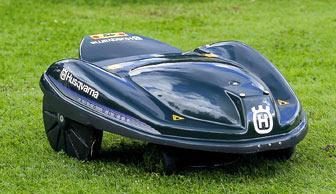
\includegraphics[width=0.4\textwidth]{Cortacesped}\\
  \caption{Robot cortacésped Automower Husqvarna}\label{fg:cortacesped}
\end{figure}

Los robots aspiradores (figura \ref{fg:aspirador})  son capaces de realizar la limpieza de todo tipo de suelos. Suelen constar de dos ruedas traseras motrices y una rueda delantera directriz. Hay modelos básicos que se mueven de forma aleatoria, sin cubrir normalmente la totalidad del espacio a limpiar, y modelos avanzados que incorporan las últimas técnicas de mapeo para lograr una alta eficiencia de funcionamiento.

\begin{figure}[hbt]
  \centering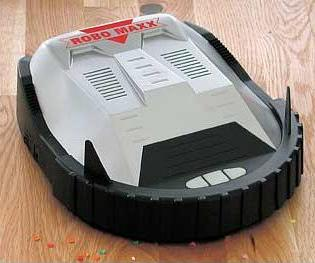
\includegraphics[width=0.4\textwidth]{aspirador}\\
  \caption{Robot aspirador RoboMaxx }\label{fg:aspirador}
\end{figure}

Los \emph{rovers} constan de un cuerpo central que se desplaza sobre seis ruedas y tienen una cabeza y un cuello para que las cámaras puedan tener una mejor perspectiva (figura \ref{fg:rover}). Estas cámaras se utilizan para la construcción de mapas que les permitan guiarse por el territorio así como para enviar imágenes a la Tierra. Estos robots también cuentan con un un brazo robótico y un gran número de sistemas térmicos, además de los sistemas de baterías y de comunicaciones.

\begin{figure}[hbt]
  \centering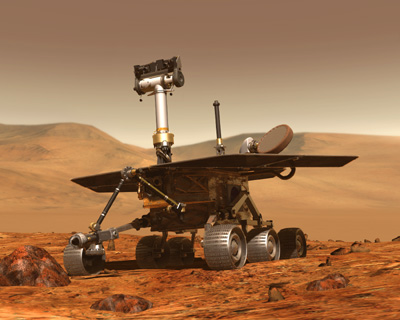
\includegraphics[scale=0.5]{MarsRover2}\\
  \caption{Rover sobre la superficie de Marte}\label{fg:rover}
\end{figure}

Los rovers \emph{Spirit} y su ''gemelo''  \emph{Opportunity} aterrizaron en el planeta rojo el 4 y el 25 de enero de 2004, respectivamente. Tienen una capacidad de movilidad mucho mayor que su antecesor el rover \emph{Pathfinder}.

Los robots guía son un tipo de robots móviles que han de tener amplio conocimiento sobre su entorno. Sus requisitos primordiales están orientados a la interacción con las personas, pero también es imprescindible en ellos un buen sistema de navegación que les permita desplazarse de forma autónoma en exposiciones, ferias y museos. Uno de estos robots es \emph{Urbano} (ver los apartados \ref{UrbanoProject}, página \pageref{UrbanoProject},  y \ref{Urbano}, página \pageref{Urbano}, así como el Anexo \ref{B}), un robot inteligente que ha sido empleado en el presente proyecto.

%---------------------------------------------------------------------------------------------------------------
\section{Antecedentes}

En el grupo de Control Inteligente de la Universidad Politécnica de Madrid, en el cual se ha realizado este proyecto, trabaja un equipo de profesores e ingenieros con elevada experiencia en el campo de los robots móviles.

\subsection{Proyectos previos}
Los proyectos dentro de esta área que más significativamente han contribuido al nivel alcanzado se describen a continuación por orden de antigüedad. En la siguiente sección se describirá el hardware de los robots empleados.

\subsubsection{Panorama (1989-1993)}
Financiado por la Unión Europea (Proyecto ESPRIT 2483), consiste en la elaboración de un sistema avanzado de percepción y navegación para vehículos industriales dentro de entornos parcialmente estructurados y parcialmente conocidos. El proyecto estuvo orientado a demostrar la viabilidad de sistemas de transporte autónomos que pudieran sustituir a vehículos controlados por conductor en un amplio rango de aplicaciones (figura \ref{fg:panorama}).

\begin{figure}[hbt]
  \centering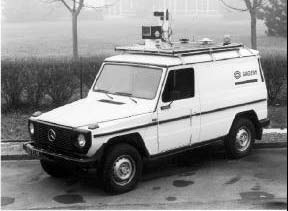
\includegraphics[width=0.5\textwidth]{Panorama}\\
  \caption{Proyecto Panorama}\label{fg:panorama}
\end{figure}


\subsubsection{RM-III (1994-1996)}
Sistema central de control para un sistema industrial de transporte basado en múltiples robots móviles autónomos dotados de inteligencia (figura \ref{fg:RM-III}). Los vehículos tienen un alto grado de autonomía que les permite evitar obstáculos y buscar en cada caso el mejor camino a seguir. Los obstáculos pueden ser tanto fijos como móviles, con lo que la dificultad aumenta. Un componente adicional en la autonomía de los vehículos lo constituye su capacidad para gestionar el nivel de carga de sus baterías, trasladándose y conectándose automáticamente a los puntos de suministro de energía al considerarlo conveniente. Este proyecto fue financiado por la Comisión Interministerial de Ciencia y Tecnología y contó con la participación de UPM-DISAM y de la Universidad Carlos III.

\begin{figure}[hbt]
  \centering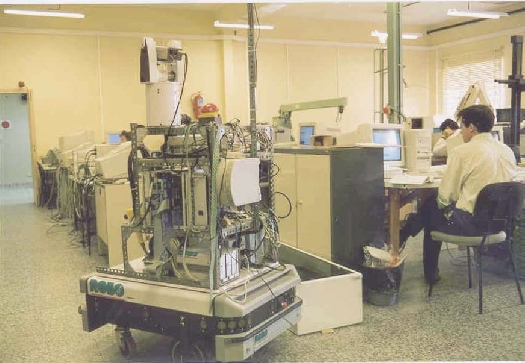
\includegraphics[width=0.5\textwidth]{Robotica3}\\
  \caption{Proyecto RM-III}\label{fg:RM-III}
\end{figure}


\subsubsection{EVS (1996-1999)}
Desarrollo de un entorno de ingeniería para facilitar el diseño y la implementación de sistemas autónomos distribuidos con aplicación en robótica móvil y en procesos continuos. Este entorno proporciona herramientas para el prototipado rápido y la experimentación, por medio de un sistema de realidad virtual que modela el sistema en desarrollo y su entorno (figura \ref{fg:EVS}).

\begin{figure}[hbt]
  \centering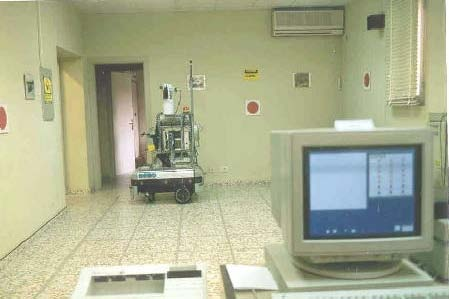
\includegraphics[width=0.5\textwidth]{EVS}\\
  \caption{Proyecto EVS}\label{fg:EVS}
\end{figure}


\subsubsection{Mobinet (1996-2000)}
Trabajo científico de un amplio conjunto de investigadores europeos en el diseño de un prototipo de robot móvil inteligente y completamente autónomo, con alta capacidad de maniobrabilidad y manipulación (figura \ref{fg:mobinet}). Destinado a servir de ayuda a personas discapacitadas, la interacción con el usuario se lleva a cabo a través de comandos de muy alto nivel. El proyecto fue financiado por la Unión Europea bajo programa TMR (Training and Mobility of Researchers).

\begin{figure}[hbt]
 \centering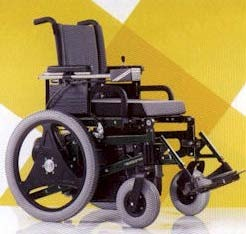
\includegraphics[scale=1.0]{MobiNet}\\
  \caption{Proyecto MobiNet}\label{fg:mobinet}
\end{figure}


\subsubsection{Blacky (2000-2001)}
Diseño de un prototipo de robot móvil para navegación en entornos parcialmente estructurados y con un elevado número de personas (figura \ref{fg:blacky}).El objetivo del proyecto es desarrollar un robot capaz de moverse en entornos complicados, tipo recintos feriales, e interaccionar con las personas que allí se encuentren.
Desde el punto de vista del control reactivo, los obstáculos no sólo no son fijos, sino que su movimiento es
totalmente imprevisible. Desde el punto de vista de la localización, se empleaba un sistema de marcas fijas en las paredes. El robot se encuentra con bastante frecuencia totalmente rodeado por personas, lo que complicaba la determinación de su posicionamiento.

\begin{figure}[hbt]
  \centering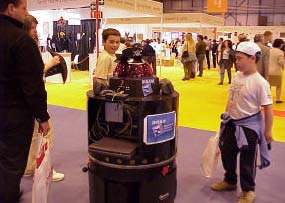
\includegraphics[width=0.5\textwidth]{Blacky}\\
  \caption{Proyecto Blacky}\label{fg:blacky}
\end{figure}


\subsubsection{WebFair (2001-2004)}
Proyecto Europeo Ref: IST-2000-29456.

Desarrollo y validación de un sistema de tele-presencia basado en robots móviles, capaz de facilitar el acceso de individuos a grandes exhibiciones y ferias comerciales a través de Internet. La construcción de mapas y demás pruebas se realizaron en el Castillo de Belgioso, Italia, dedicado a la celebración de exposiciones (figura \ref{fg:WebFair}).

\begin{figure}[hbt]
  \centering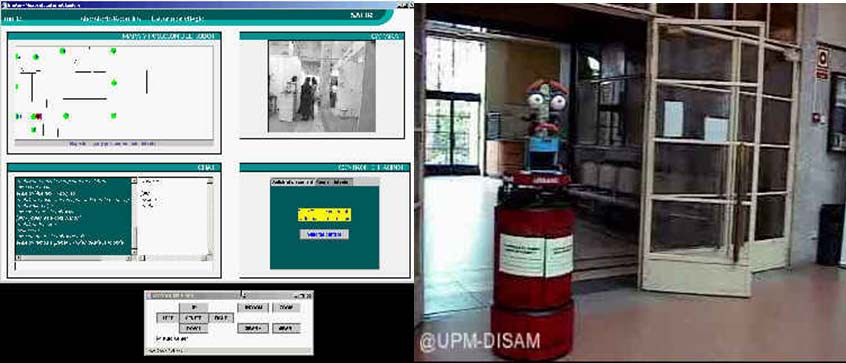
\includegraphics[width=0.5\textwidth]{WebFair}\\
  \caption{Proyecto WebFair}\label{fg:WebFair}
\end{figure}

\subsubsection{Guido (2004)}
Sistema de navegación robusto para un robot de la empresa Haptica que sirva de ayuda a la movilidad de personas débiles o con problemas de visión (figura \ref{fg:guido}). Un punto a destacar entre las mejoras introducidas es la utilización de la información proporcionada por los bordes de segmentos del mapa, lo cual evita redundancias y permite así disminuir el coste computacional \cite{RodriguezLosada05}. Muy buenos resultados en casos reales empleando un ordenador portátil auxiliar.

\begin{figure}[hbt]
  \centering\includegraphics[scale=0.8]{GuidoProject}\\
  \caption{Proyecto Guido}\label{fg:guido}
\end{figure}

\subsubsection{Urbano(2001-2004)}\label{UrbanoProject}
Proyecto de investigación nacional Ref: DPI2001-3652C0201.

Proyecto financiado por el Ministerio de Ciencia y Tecnología y supervisado por la Ciudad de las Artes y las Ciencias de Valencia (CACSA), donde el robot se ha probado con éxito (figura \ref{fg:urbano}). El módulo de navegación fue desarrollado por Diego Rodríguez-Losada en el marco de su Tesis Doctoral \cite{Rodriguez-Losada04}.

\begin{figure}[hbt]
  \centering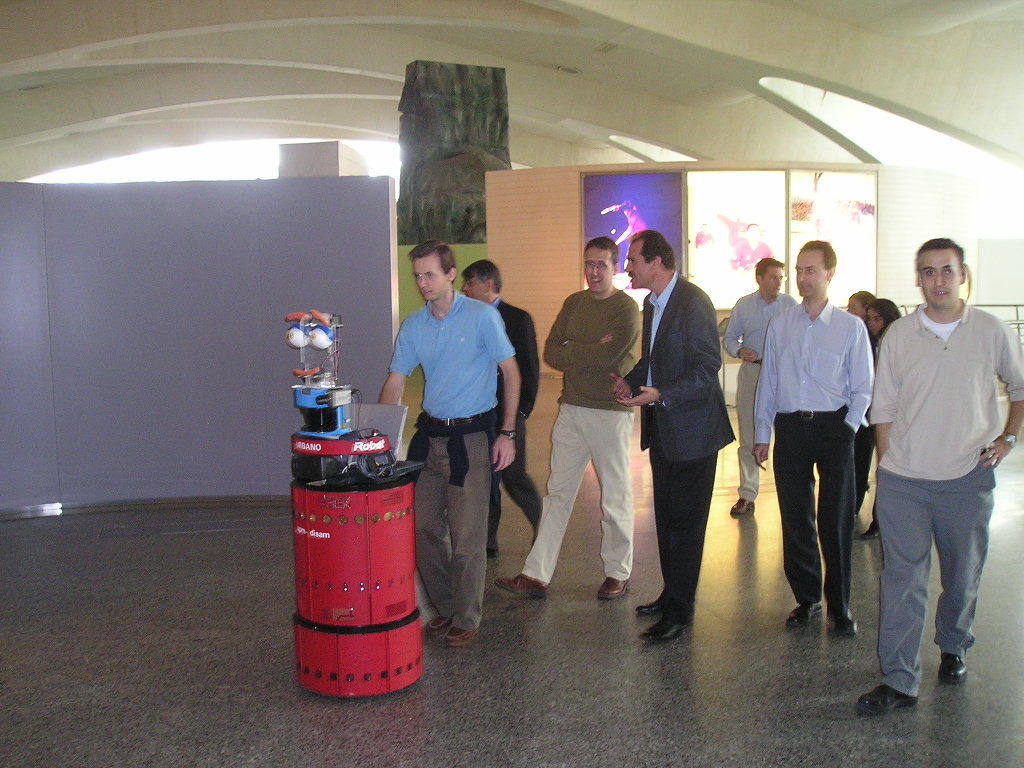
\includegraphics[width=0.5\textwidth]{UrbanoValencia}\\
  \caption{Proyecto Urbano}\label{fg:urbano}
\end{figure}

\clearpage

\subsubsection{RobInt (2004-2007)}
Ref: DOI 2004-007908C0201.

Modelado, diseño de una tecnología de diseño e implementación de comportamientos inteligentes en robots guía. Se trata de un proyecto financiado por el Ministerio de Ciencia y Tecnología que da continuidad al proyecto Urbano introduciendo mejoras en los módulos de navegación, consciencia y emociones, conocimiento y diálogo.

%%%%%%%%%%%%%%%%%%%%%%% 	aqui %%%%%%%%%%%%%%%%%%%%

\subsection{Robots}

\subsubsection{ROBUTER}
Fabricado por Robosoft, consiste en una plataforma con elevada capacidad sensorial pensada para trabajo de experimentación. El modo de locomoción es diferencial y cuenta con un computador principal de Motorola con sistema operativo Albatros. Tiene también un computador secundario Sun Sparc. Los sensores de proximidad que posee son 24 sensores de ultrasonidos. También presenta capacidad de visión y Wireless Ethernet. Este robot se utilizó en los proyectos RM-III y EVS.

\begin{figure}[h]
  % Requires \usepackage{graphicx}
  \centering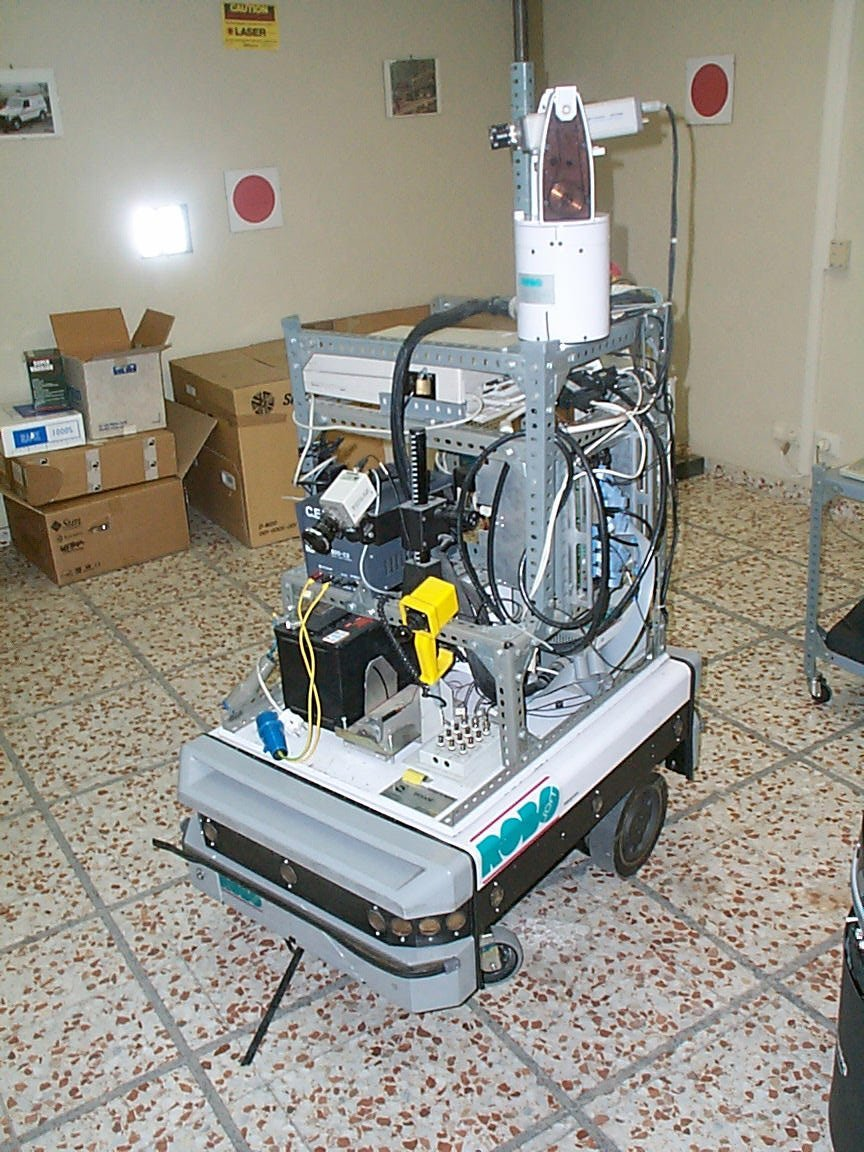
\includegraphics[scale = 0.2]{ROBUTER}\\
  \caption{Robot ROBUTER}\label{fg:robuter}
\end{figure}

\subsubsection{BLACKY}
Plataforma MRV-4 de Denning Branch Int. Robotics dotada de un PC Pentium con sistema operativo Linux y un láser rotatorio para la localización con balizas reflectantes. También posee 24 sensores de ultrasonidos y Ethernet Wireless radio. Es el robot utilizado en el proyecto del mismo nombre.

\begin{figure}[h]
  % Requires \usepackage{graphicx}
  \centering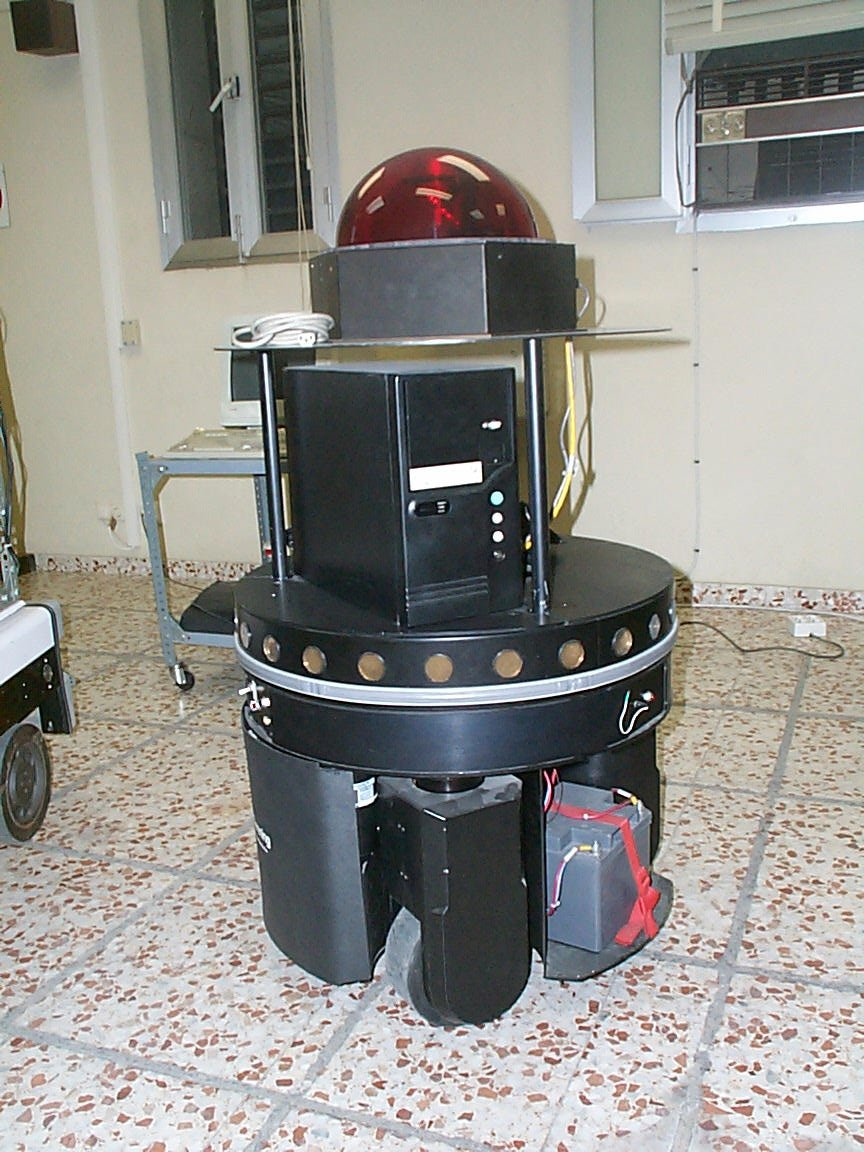
\includegraphics[scale = 0.2]{MRV-4}\\
  \caption{Robot BLACKY}\label{fg:mrv4}
\end{figure}

\subsubsection{URBANO}\label{Urbano}
Plataforma B21r del fabricante iRobot. El computador base es un PC Pentium con sistema operativo Linux; el computador secundario es un PC Pentium con Windows. Dispone de un láser SICK LM300 para la localización. También posee 24 sensores de ultrasonidos e infrarrojos y Ethernet Wireless radio. En DISAM-UPM se han desarrollado una cabeza y un brazo con los que el robot puede hacer gestos e interaccionar con personas. Este robot se ha empleado en los proyectos WebFair, Urbano y RobInt.

\begin{figure}[h]
  % Requires \usepackage{graphicx}
  \centering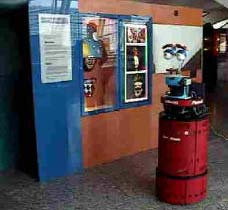
\includegraphics[scale=1]{Urbano}\\
  \caption{Robot Urbano}\label{fg:b21r}
\end{figure}

Dado que este robot ha sido asimismo utilizado en el desarrollo de este proyecto, puede consultarse más información sobre él en el Anexo B.

\subsubsection{GUIDO}
Guido es un robot de cuatro ruedas con dos motores para hacer girar las dos delanteras, pero ha de ser empujado para moverse \cite{Rodriguez-Losada05}. Tiene un sensor láser para percibir el entorno y en el manillar hay un sensor de medida de fuerza para detectar el comando de giro. El computador de a bordo es un PC104 300~MHz Geode con 32~MB de disco duro y 32~MB de RAM, con sistema operativo Haptica-TinyDCLinux. Tiene disponible un puerto Ethernet para las comunicaciones y se alimenta a 24V suministrados por cuatro baterías.

\begin{figure}[h]
  % Requires \usepackage{graphicx}
  \centering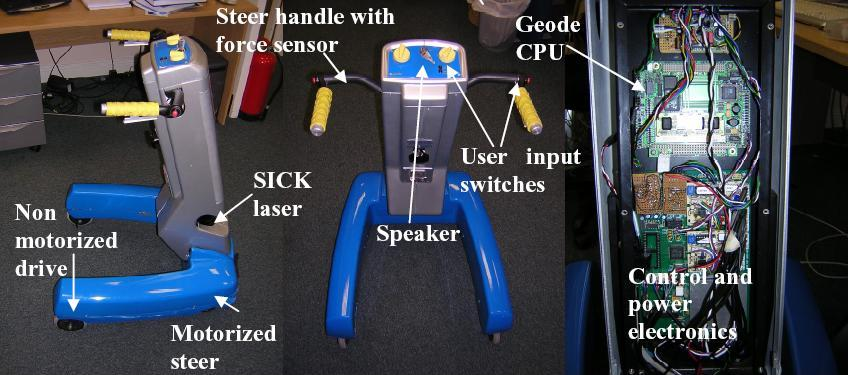
\includegraphics[scale=0.4]{Guido1}\\
  \caption{Robot Guido}\label{fg:guido1}
\end{figure}


\section{Marco del proyecto}
Este proyecto se ha llevado a cabo bajo beca de colaboración concedida por el Ministerio de Educación y Ciencia en el Departamento de Automática, Ingeniería Electrónica e Informática Industrial de la Escuela Técnica Superior de Ingenieros Industriales de la Universidad Politécnica de Madrid, dentro del grupo de Control Inteligente.

\section{Objetivos del proyecto}
El objetivo del proyecto consiste en la realización de un sistema de navegación para un robot móvil. Se ha trabajado en control de movimiento, planificación de trayectorias, control reactivo, localización y construcción de mapas.

\section{Alcance del proyecto}
Los principales elementos de trabajo en este proyecto son los siguientes:
\begin{itemize}
  \item \textbf{Formación previa.} En primer lugar se requería un asentamiento de conocimientos sobre programación y algorítmica, el aprendizaje de C++ y Visual C++. Posteriormente fue necesaria la comprensión de la base de software de navegación existente. Otra parte importante era la puesta en funcionamiento del robot Pioneer P3AT y el estudio de las librerías de la distribución Aria.
  \item \textbf{Desarrollo del control de movimiento.} Programación de un regulador proporcional con planificación de ganancia, empleando tanto los parámetros de Urbano como los correspondientes al Pioneer. Generación de una trayectoria suave en los puntos de paso de una trayectoria definida. Algoritmo para evitar desviaciones sobre la trayectoria programada. Control reactivo: deformación de la trayectoria por la presencia de obstáculos y paredes cercanas al camino inicial a seguir por el robot.
  \item \textbf{Localización y construcción de mapas.} Estudio del filtro de Kalman y del filtro extendido de Kalman (EKF). Aplicación a la la localización del robot a partir de los puntos de medida proporcionados por el láser. Modificación del modelo para el caso de disponer únicamente de medidas de distancia, que no se utiliza debido a su peor comportamiento. Programación de las fases de predicción y corrección del algoritmo. Análisis del coste computacional y reducción del tiempo de procesamiento. Obtención y actualización de mapas de puntos a partir de los datos registrados por el láser. Utilización de mapas ya realizados para efectuar la localización. Borrado de los puntos correspondientes a obstáculos dinámicos del mapa que se encuentren cercanos a la posición del robot en cada momento.
      Con el Pioneer sólo es utilizable la parte del proyecto relativa al control de movimiento, planificación de trayectorias y control reactivo ya que al no poderse utilizar el láser no era posible realizar tareas de localización.
  \item \textbf{Integración.} Funcionamiento conjunto e intercambio de información entre los componentes anteriormente indicados.
  \item \textbf{Pruebas.} Pruebas de funcionamiento en modo simulación y con los robots reales. Corrección, depuración y posibles mejoras a partir de los resultados de dichas pruebas.

  Paralelamente se iba desarrollando un cuadro de diálogo para facilitar la ejecución y la selección de opciones en la misma.
\end{itemize}

% -*- coding: utf-8 -*-

\chapter{Estado del Arte}

\section{Navegación, planificación de trayectorias y control reactivo}
Un aspecto esencial de un robot móvil es su capacidad de navegación. Sin entrar en profundidad en la cinemática implicada en el movimiento de diferentes tipos de robots móviles, ha de tenerse en cuenta que ésta limita significativamente las posibles configuraciones que puede adoptar un robot para moverse entre dos determinados puntos. El término \emph{trayectoria} se diferencia del de \emph{camino} en que incorpora la dimensión tiempo. Así, mientras que en un camino se tiene una serie discreta de puntos o configuraciones, en una trayectoria se asocia a cada uno de ellos una velocidad. No obstante, cuando se hace referencia a la planificación, es corriente el empleo de ambos conceptos indistintamente.

\subsection{Control de movimiento}
El desplazamiento del robot entre dos puntos se realiza mediante lo que se conoce como \emph{motion control}. Existen diferentes técnicas para afrontar esta tarea, distinguiéndose entre control en bucle abierto o control con realimentación\cite{Siegwart04}.
\subsubsection{Control en bucle abierto}
Consiste en el seguimiento de una trayectoria definida por un perfil de puntos o velocidades en función del tiempo. El mayor inconveniente que presenta es la alta probabilidad de que el robot no llegue a su destino si por algún motivo se encuentra en un lugar distinto al previamente esperado para un cierto momento. Además, precalcular una trayectoria posible no resulta sencillo en muchos casos. Otra de sus desventajas es que suele basarse en movimientos de giro o avance puros, y con frecuencia da lugar a movimientos algo bruscos.
\subsubsection{Control con realimentación}
Una manera más apropiada de tratar el control de movimiento de un robot móvil es el control mediante \emph{feedback} de su posición. Con un controlador de este tipo, la planificación de trayectorias se reduce a la obtención de una serie de puntos intermedios que determinen el camino a seguir entre los puntos origen y destino.

\subsection{Aptitudes para la navegación: planificación y reacción}
En navegación de alto nivel juegan un papel fundamental las habilidades de planificación y reacción del robot. Ambos sistemas son igualmente importantes y han de integrarse adecuadamente. De nada sirve que el robot disponga de un conjunto de acciones a realizar para alcanzar un objetivo dado (plan), si durante la ejecución del mismo se encuentra con condiciones no previstas a las que no sabe cómo hacer frente. Tampoco tiene sentido que el robot sea capaz de reaccionar ante diferentes circunstancias si no puede guiarse para llegar al destino deseado. La solución teórica ideal lleva a la fusión de ambos conceptos, de modo que constantemente se elabora o actualiza un plan que reaccione en tiempo real a la información más inmediata que se tenga para describir el entorno.

Se dice que el sistema de un robot es completo si y sólo si para todos los posibles problemas que puedan encontrarse (diferentes estados de partida, mapas o destinos\ldots), cuando exista alguna trayectoria entre el estado inicial y el final, el sistema llegará al estado final. Por lo tanto, si un sistema es incompleto significa que existe al menos un problema que tiene solución para el cual el sistema no encuentra solución. Siendo una propiedad enormemente difícil de conseguir, a menudo se renuncia a la completitud por razones de coste computacional.

\subsubsection{Planificación de trayectorias}
La planificación de trayectorias se lleva a cabo en la mayoría de los casos en una representación formal denominada \emph{espacio de configuración}. Para un robot con $k$ grados de libertad, cada uno de sus posibles estados o configuraciones se describirá con $k$ valores reales: $q_{1},q_{2}...,q_{k}$. El vector que contenga esas $k$ coordenadas podrá considerarse como un punto en un espacio de dimensión $k$ que recibe el nombre de espacio de configuración $C$ del robot. En el caso de que el robot se mueva en las cercanías de algún obstáculo, han de evitarse las colisiones con él, lo cual puede complicarse mucho en el espacio físico. Sin embargo, en el espacio de configuración la resolución del problema es directa si se define el \emph{espacio de configuración de obstáculos} $O$ como el subespacio de $C$ en el que el robot choca contra algún objeto. El subespacio libre en el que el robot puede moverse con seguridad será la diferencia $F = C-O$.

Generalmente, se considera al robot móvil como un simple punto. En consecuencia, el espacio de configuración es fácilmente manejable por ser plano con ejes $x$ e $y$. Una importante consideración a realizar es el hecho de que al reducirse el robot a un punto, habrá que aumentar el tamaño de los obstáculos en la medida del radio del robot.

Una vez introducido este concepto, se distinguen tres estrategias principales para efectuar la planificación de trayectorias básica:
\begin{itemize}
  \item \emph{Mapa de líneas}: basado en identificar rutas en el espacio libre. Destacan los métodos del \emph{Gráfico de visibilidad } y del \emph{Diagrama de Voronoi}.
  \item \emph{Descomposición en celdillas}: a partir de una mapa de celdillas se clasifican éstas en libres y ocupadas y se crea un grafo de conectividad entre celdas libres adyacentes (ver \ref{mapas}).
  \item \emph{Campo de potencial}: consiste en imponer una adecuada función matemática sobre el espacio. Permite obtener la \emph{fuerza} sobre el robot (que se traducirá en una velocidad) como resultado de potenciales de atracción y repulsión.
\end{itemize}

Las trayectorias generadas por estos algoritmos pueden ser mejoradas en relación a distintos criterios. Por ejemplo, puede resultar interesante suavizar los ángulos en las trayectorias previas mediante arcos de circunferencia (como se implementa en el presente proyecto) o interpolación cuadrática. Estas técnicas de perfeccionamiento son también un componente relevante del término planificación de trayectorias.

\subsubsection{Control reactivo}
El control reactivo tiene como principal propósito evitar que el robot pueda chocar con algún obstáculo en el seguimiento de la trayectoria previamente hallada. Para ello existen diversos algoritmos que modifican estas trayectorias en función de los objetos detectados por las medidas que le llegan al robot procedentes de los sensores estereoceptivos. La presencia de obstáculos en una trayectoria obtenida mediante planificación sobre un mapa del entorno puede deberse a errores en la localización, a imprecisiones en el mapa utilizado o a obstáculos dinámicos no contemplados en dicho mapa.

Algunas soluciones (por ejemplo la mostrada en \cite{Feiten94}) consisten en calcular un conjunto de comandos de giro o de variación de la velocidad a aplicar al robot en función de lo que éste percibe a través de sus sensores. También se ha afrontado la tarea de esquivar obstáculos mediante controladores basados en lógica borrosa.

Un nuevo enfoque, efectivo y genérico, es el que se presenta en \cite{Lamiraux04}. A partir de un camino inicial libre de obstáculos, se trata de ir deformándolo iterativamente cuando se encuentran obstáculos próximos, siguiendo para ello un criterio de optimización. El camino deformado debe apartarse de los obstáculos, cumplir las restricciones cinemáticas de movimiento (lo que complica significativamente el problema en el caso de robots no holónomos) y mantener las mismas configuraciones inicial y final que el camino original. En el artículo se establece un marco teórico en el que la deformación del camino inicial se modela como un sistema dinámico dentro del algoritmo que controla el proceso.

También cabe mencionar que existen otros algoritmos de control reactivo que podrían considerarse más avanzados por tener en cuenta la velocidad de los obstáculos detectados. No obstante, emplean modelos excesivamente sencillos del robot y los obstáculos que no suelen conducir a un buen comportamiento práctico.

Por último, hay trabajos recientes que se centran en resolver el problema en escenarios complejos, con un alto grado de ocupación o dinámicos. Para ello, se basan en estrategias de “divide y vencerás” y posteriormente aplican diferentes técnicas de control reactivo. En \cite{Minguez04} se explica una metodología que, a nivel simbólico, consiste en identificar situaciones para posteriormente aplicar una determinada acción en cada caso. Una vez definidas las posibles situaciones (a partir de las posiciones relativas de robot, obstáculos y destino) así como las acciones asociadas a las mismas, se realiza una implementación geométrica particular.

\section{Localización y construcción de mapas con un robot móvil}
Uno de los mayores problemas que conciernen a la navegación de robots móviles consiste en la determinación de su localización con un elevado grado de precisión. Para cumplir con el objetivo de autonomía no basta con situar el robot en un sistema de referencia global sino que es imprescindible conocer su posición relativa tanto respecto a posibles obstáculos móviles como respecto al modelo estático de su entorno. Para ello, existen diferentes alternativas utilizando mapas que, o bien se introducen previamente al robot, o bien se elaboran a medida que el mismo se mueve por un determinado lugar. Esta segunda opción empieza a desarrollarse a finales de los años 80. En un principio se desacoplaron los problemas de construcción del mapa y de la localización del robot en el mismo; pronto se descubriría que la solución rigurosa requiere tratar ambos aspectos al mismo tiempo en lo que se conoce como SLAM (Simultaneous Localization and Mapping). La solución al problema SLAM está considerada como pieza clave en la búsqueda de la completa autonomía de un robot móvil y concentra los principales esfuerzos de investigación de grupos de robótica móvil de todo el mundo que han conseguido importantes avances y continúan intentando resolver dicho problema.

El origen de las dificultades en la localización y la construcción de mapas se deriva de la existencia de ruido en las medidas de los sensores y en las limitaciones en el rango de las mismas. Un poco más en profundidad, los principales factores que impiden que el proceso sea más sencillo son los siguientes:
\begin{itemize}
  \item  Las observaciones se obtienen con respecto al sistema de referencia propio del robot, cuya posición viene afectada de un cierto grado de incertidumbre inherente a la odometría. Así, la imprecisión en las observaciones se añade a la ya existente en la posición del robot y se complica extremadamente la minimización de los errores.
  \item En multitud de casos es necesaria la representación de mapas de tamaño grande, lo cual supone un mayor coste computacional y una mayor imprecisión en la odometría según aumentan los desplazamientos del robot.
  \item Los entornos suelen ser dinámicos, sobre todo en el caso de robots guía o domésticos. Si se considera que las observaciones corresponden a puntos fijos representados con carácter permanente en el mapa se simplifica el problema, pero se tienen discrepancias con la realidad. Una aproximación parcialmente eficiente consiste en ir borrando objetos transitorios del mapa a lo largo del tiempo, tratándolos a modo de ruido. El rápido avance de la visión artificial y el desarrollo de dispositivos sensores que diferencien entre obstáculos móviles y estructuras estáticas dentro de un marco de referencia móvil permitirán notables mejoras en este aspecto.
  \item La asociación de las observaciones con los objetos del mapa puede resultar compleja si éstos son parecidos entre sí. En muchos casos no puede efectuarse la correspondencia de forma determinista y ha de emplearse una formulación probabilista. Algunas mejoras para abordar este problema y descartar las asociaciones erróneas se han presentado en \cite{Rodriguez-Losada07}.
  \item Los entornos son tridimensionales pero contemplar este aspecto introduce un mayor grado de complejidad y ha de tenerse en cuenta que generalmente los sensores están configurados para una percepción plana horizontal. Aunque existen algunos trabajos en la representación de mapas tridimensionales, la mayor parte de los algoritmos más empleados hasta el momento aceptan la hipótesis de bidimensionalidad del entorno. El paso a modelos en tres dimensiones es uno de los próximos objetivos a seguir (capítulo 7).
\end{itemize}

\subsection{Tipos de mapas}\label{mapas}
Cuanto mayor sea la complejidad del mapa a emplear, mayor será la complejidad computacional de su construcción, de la localización y de la navegación. La precisión del mapa vendrá condicionada en cada caso por la precisión que se necesite en el movimiento del robot y por la precisión de los sensores de que se disponga.

Se establecen tres niveles posibles de representación en la definición de un mapa: geométrico, topológico y semántico. Una representación completa del entorno debería incorporarlos todos pero con frecuencia las soluciones halladas se centran en uno sólo de ellos y, a lo sumo, incluyen uno o los dos restantes como mera información extra que pueda mejorar la navegación.

El nivel métrico consiste en representar las coordenadas y propiedades de los objetos del mapa. Este modelo puede a su vez ser geométrico, en el que se representan elementos discretos del entorno de modo que almacenan su parametrización geométrica, o discretizado, en el que la ocupación del entorno se analiza mediante una división del mismo.
Así, los mapas métricos geométricos representan objetos con determinadas características geométricas y diferentes grados de complejidad dependiendo de las capacidades sensoriales y de extracción de información. En la figura \ref{fg:geometricos} se muestran dos mapas geométricos que reflejan propiedades características de los entornos de interiores. En el mapa de la izquierda se representan las paredes mediante segmentos y en el de la derecha puede apreciarse que las esquinas y objetos delgados, como patas de mobiliario, se representan como puntos.

\begin{figure}[hbt]
  % Requires \usepackage{graphicx}
  \centering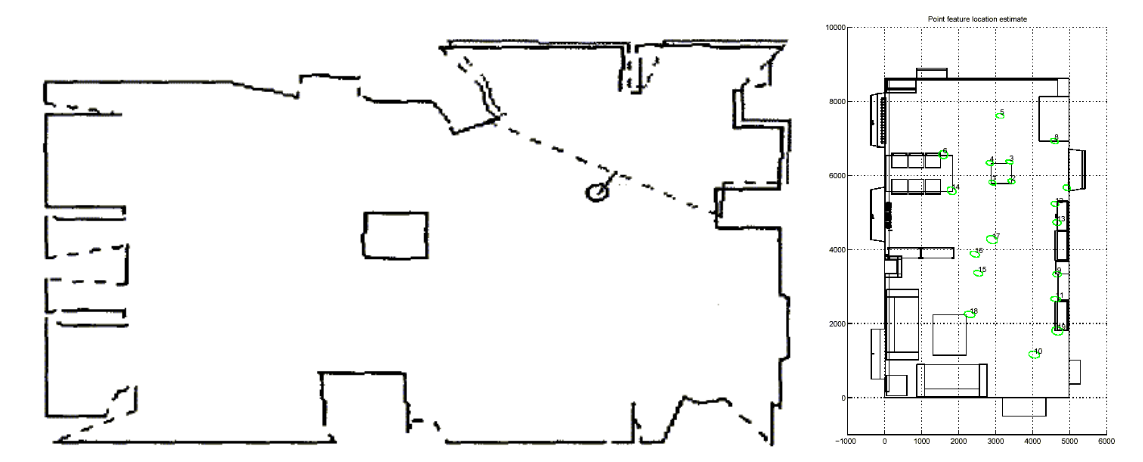
\includegraphics[width=0.5\textwidth]{mapas_geometricos}\\
  \caption{Mapas métricos geométricos}\label{fg:geometricos}
\end{figure}

Este tipo de mapas es ampliamente utilizado en entornos estructurados debido principalmente a la facilidad de visualización que ofrecen y la compacidad que presentan. Otra ventaja fundamental es la filtración de los objetos dinámicos al hacerse la extracción previa de características del entorno. Los sensores necesarios para construir estos mapas no pueden generar mucho ruido, puesto que han de permitir distinguir los diferentes elementos del entorno. Otro inconveniente a resaltar es su incapacidad para proporcionar un modelo completo del espacio que rodea al robot. Los puntos que no se identifican como características geométricas del mundo real son eliminados, con lo que para ganar en robustez y compacidad se pierde información de los sensores. Esta limitación afecta a tareas como la planificación de trayectorias y la exploración de entornos, reduciendo consiguientemente la utilidad de estos mapas en la navegación de robots móviles.

En los mapas métricos discretizados,se utiliza la información de los sensores sin segmentar y se construye una función de densidad de probabilidad de ocupación del espacio. Como ésta no puede cubrir todo el espacio de forma continua, se efectúa una descomposición en celdillas y se asigna una probabilidad a que cada una esté ocupada o libre. Esta división puede ser exacta, manteniendo las fronteras de los obstáculos como bordes de las celdillas, o mediante celdillas de dimensiones fijas que se reparten por todo el espacio \cite{Siegwart04}. En las figuras \ref{fg:exactas} y \ref{fg:fijas} pueden verse ejemplos de ambos tipos de descomposición. En la división en celdillas fijas se aprecia que un estrecho paso entre dos obstáculos puede perderse con esta representación.

 \begin{figure}[hbt]
  % Requires \usepackage{graphicx}
  \centering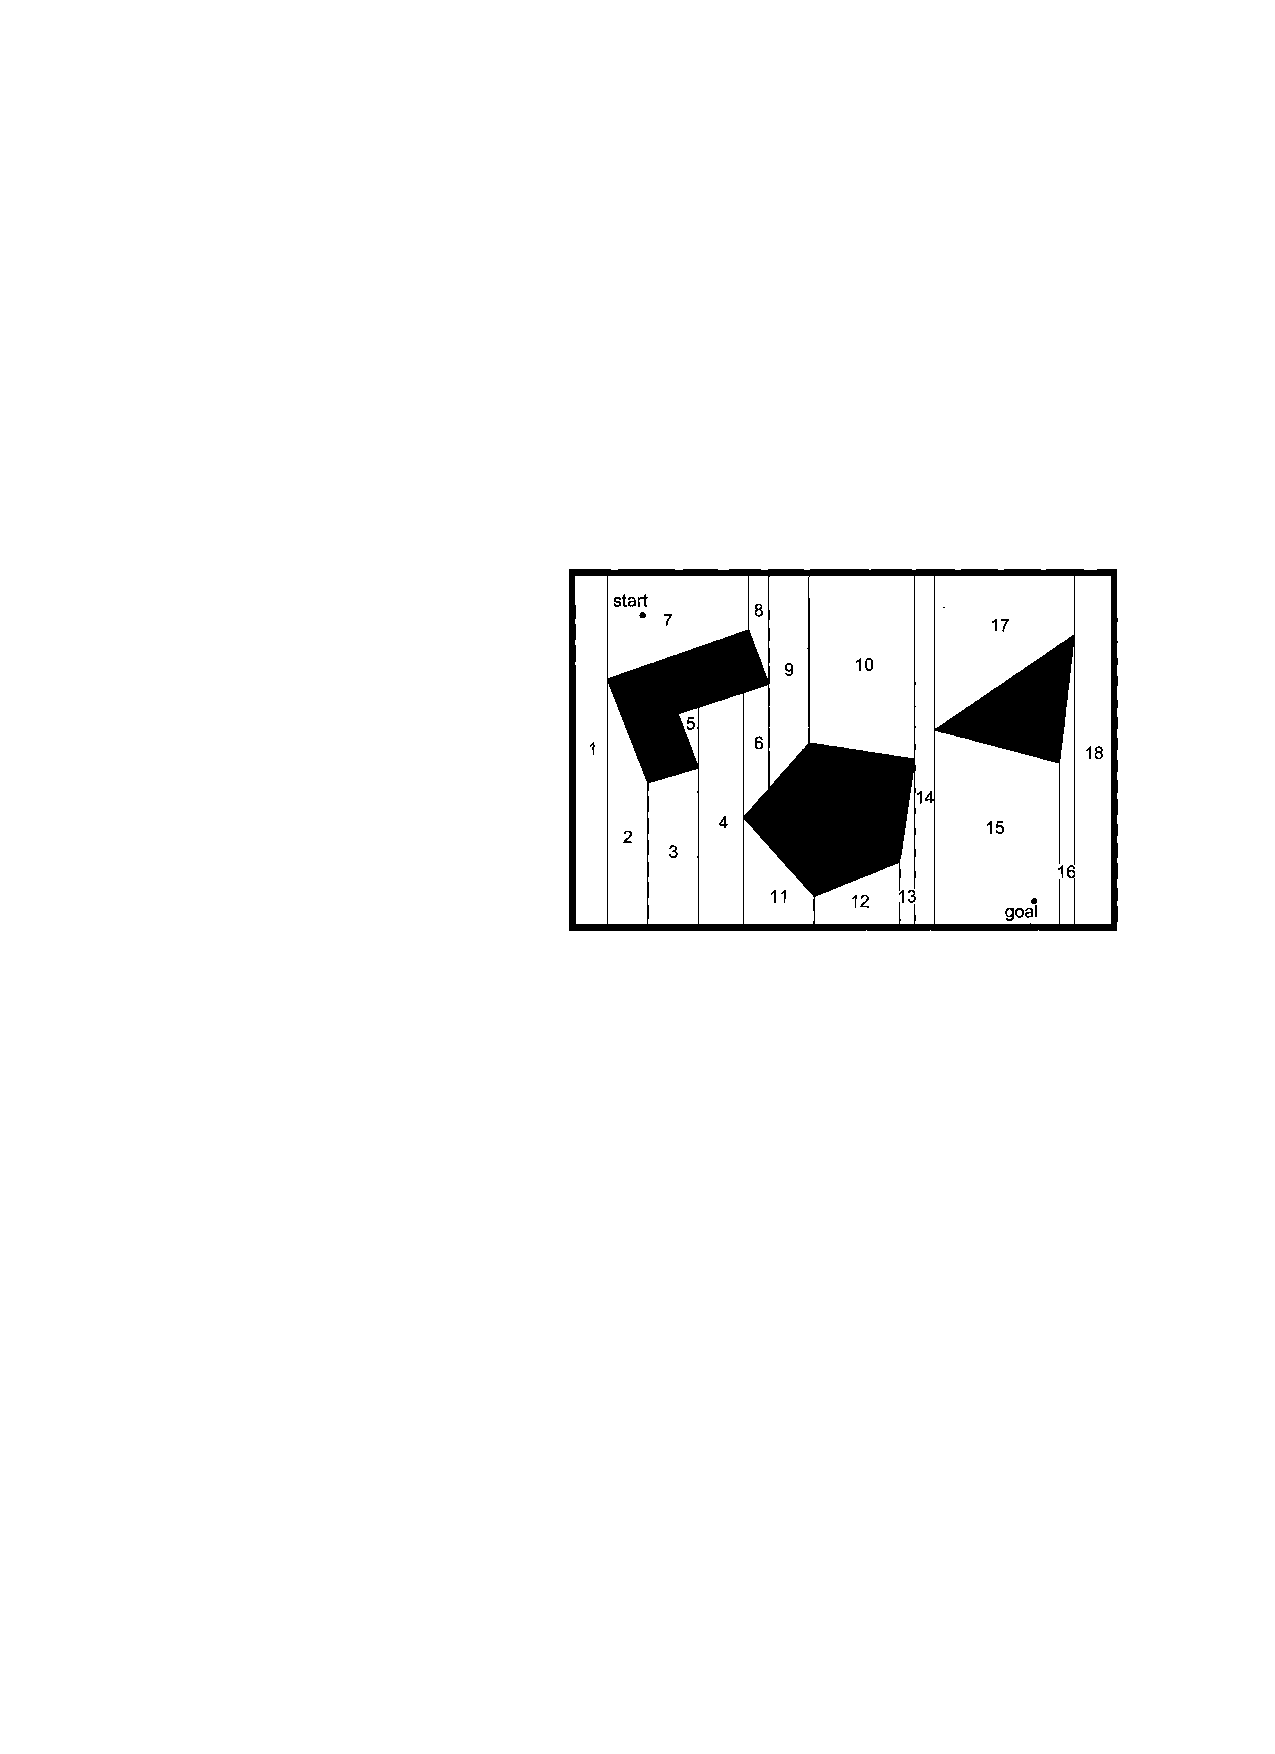
\includegraphics[width=0.5\textwidth]{celdas_exactas}\\
  \caption{Descomposición en celdillas exactas}\label{fg:exactas}
\end{figure}

\begin{figure}[hbt]
  % Requires \usepackage{graphicx}
  \centering{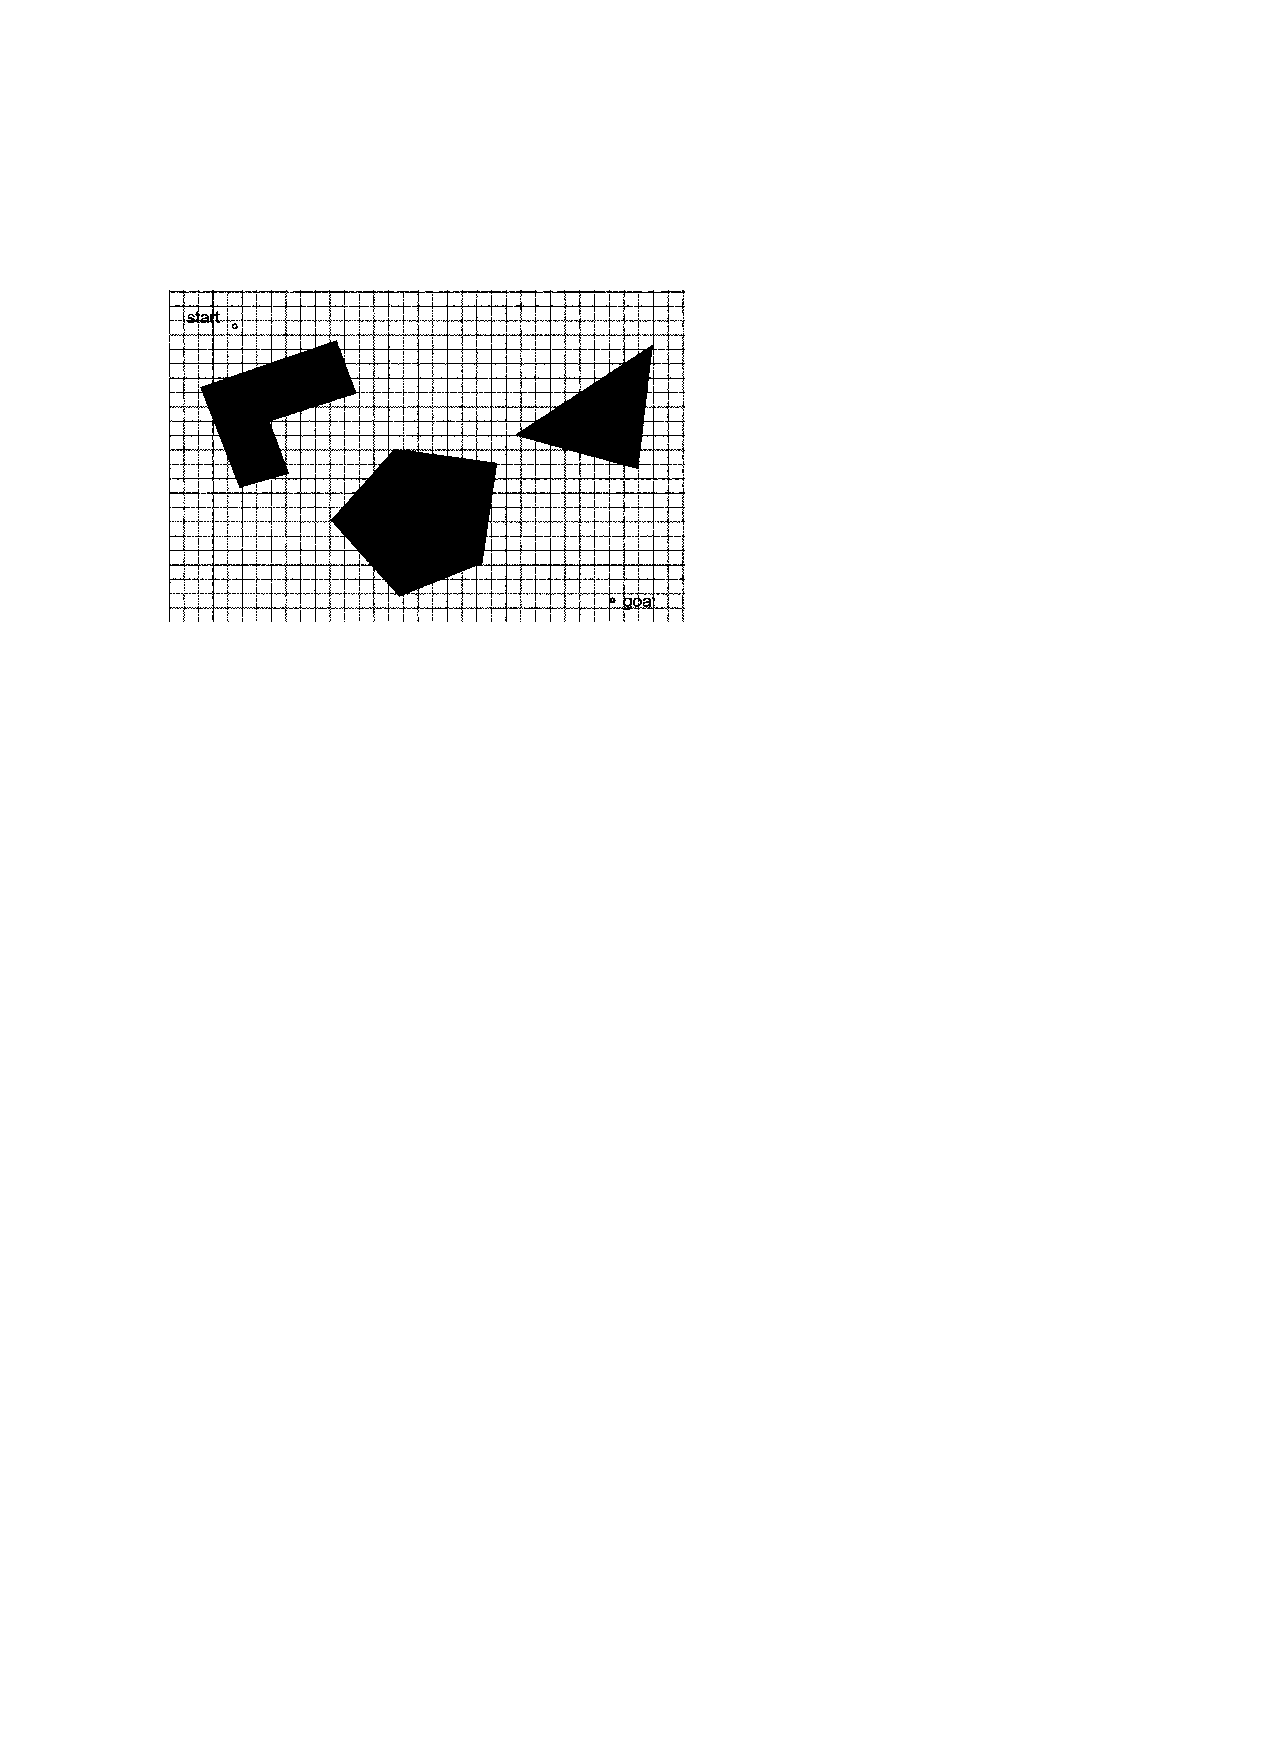
\includegraphics[width=0.4\textwidth]{celdas_fijas1}
  \hspace{0.1cm} 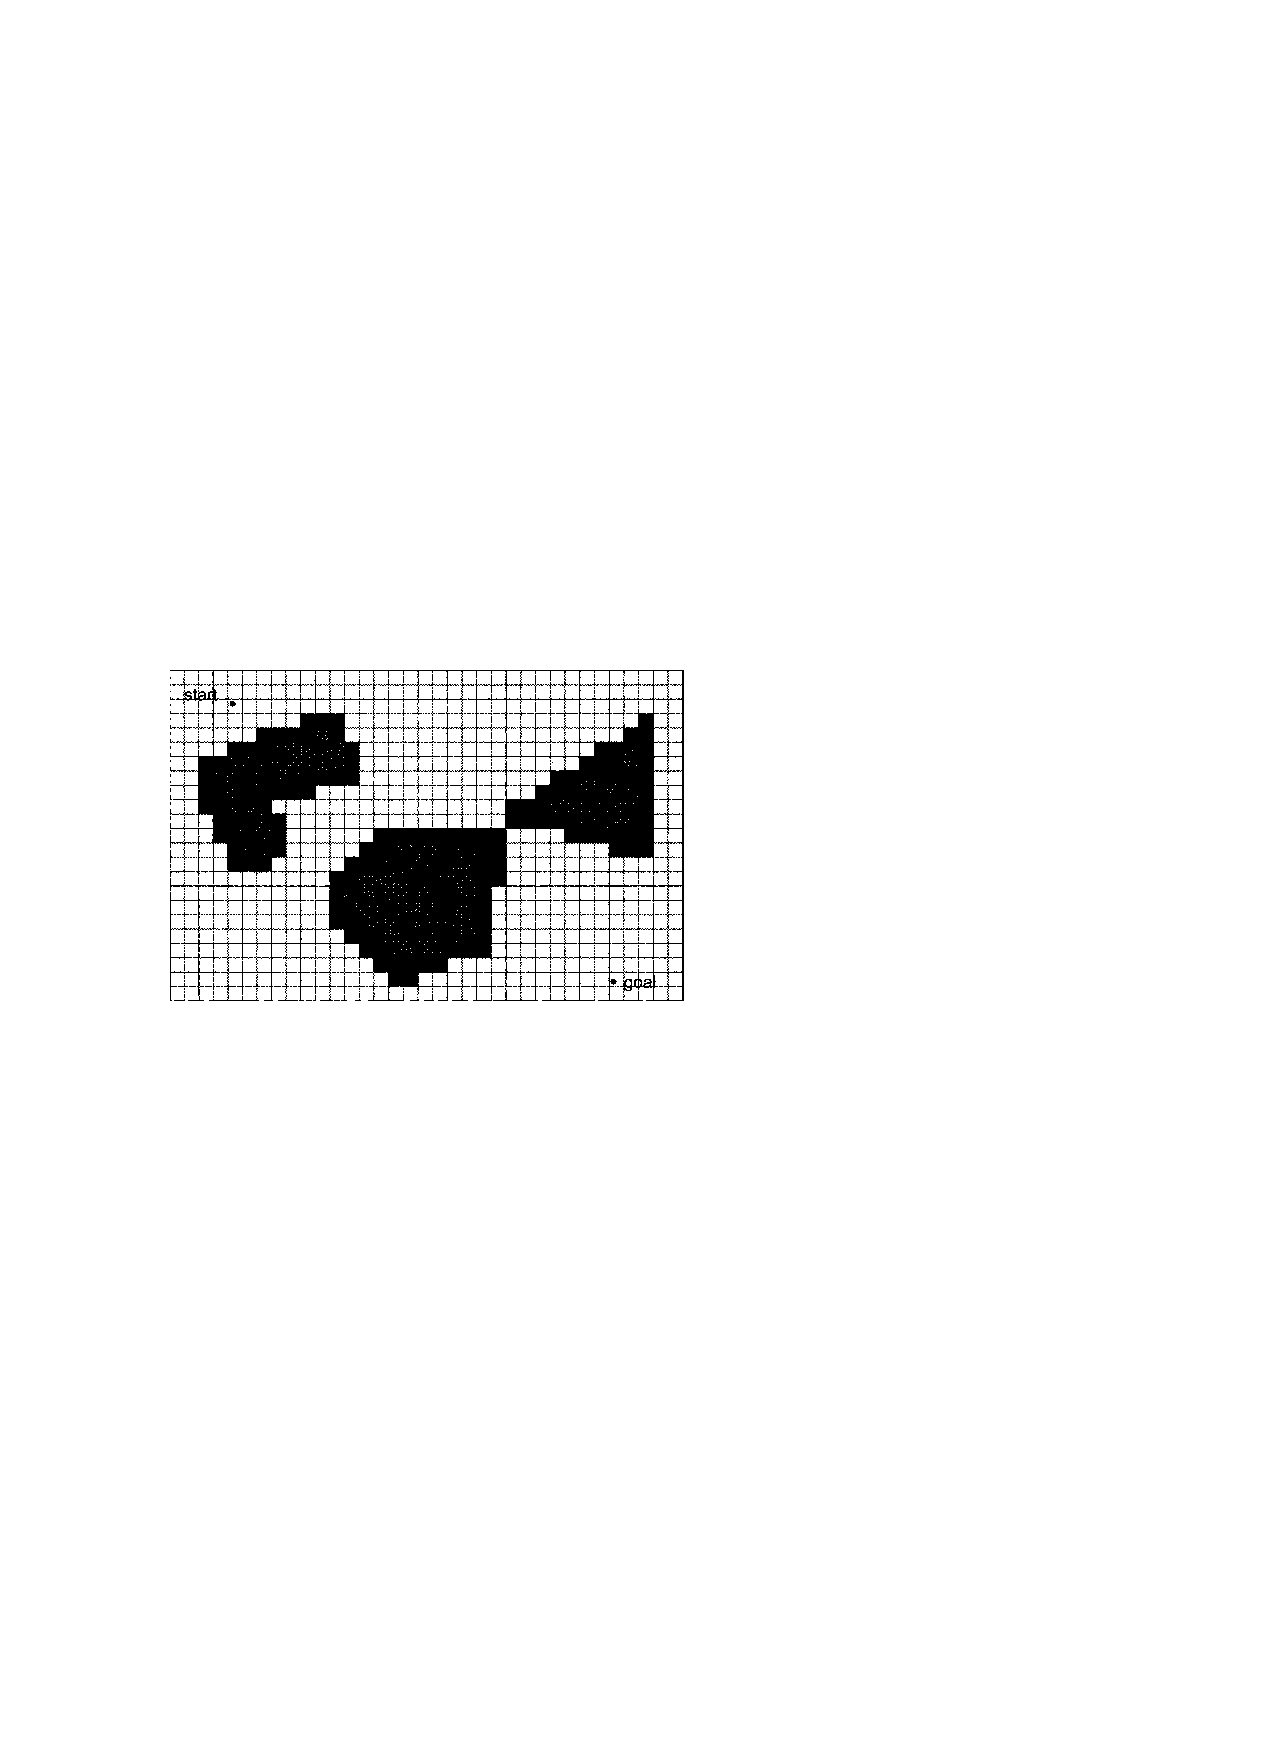
\includegraphics[width=0.4\textwidth]{celdas_fijas2}}  \\
  \caption{Descomposición en celdillas fijas}\label{fg:fijas}
\end{figure}


 En este caso no se analiza la pertenencia de cada celdilla a un objeto individual, por lo que aunque el espacio esté discretizado se logra su representación de forma continua. En la figura \ref{fg:discretizado} se puede ver un mapa discretizado o de ocupación de celdillas de un entorno con formas irregulares que haría complicada la representación geométrica.

\begin{figure}[hbtp]
  % Requires \usepackage{graphicx}
  \centering
\includegraphics[scale=0.4]{mapa_discretizado}\\
  \caption{Mapa métrico discretizado}\label{fg:discretizado}
\end{figure}

Este tipo de mapas puede precisar de una alta capacidad de almacenamiento, tanto mayor cuanta más resolución se requiera. Por otra parte, permite representaciones continuas y completas incluso a partir de datos de sensores con mucho ruido como los de ultrasonidos, lo que los hace especialmente prácticos.

El nivel de representación topológico se centra en definir nodos (en ocasiones llamados \emph{lugares distintivos}) y las conexiones entre ellos. Los mapas topológicos a menudo se elaboran a partir de mapas geométricos pero también pueden obtenerse directamente. Un concepto importante en estos modelos es el de nodos adyacentes. Los nodos adyacentes son aquellos que el robot puede alcanzar sucesivamente sin pasar por ningún otro nodo intermedio. Dentro de este nivel son muy comunes las representaciones basadas en el Diagrama de Voronoi o el Gráfico de Voronoi Generalizado (GVG)como las que se presentan en \cite{Choset01} y se muestran en la figura \ref{fg:topologicos}.

\begin{figure}[hbtp]
  % Requires \usepackage{graphicx}
  \centering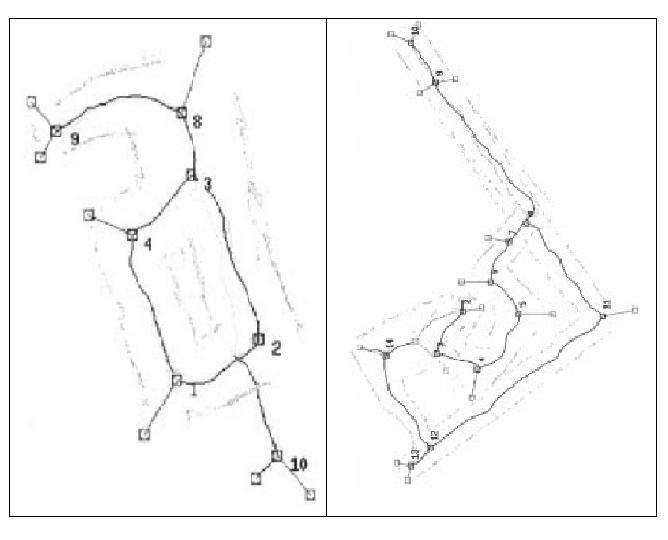
\includegraphics[scale=0.4]{mapas_topologicos}\\
  \caption{Mapas topológicos basados en el diagrama de Voronoi}\label{fg:topologicos}
\end{figure}

%El diagrama de Voronoi es también una forma de hacer frente a la planificación de trayectorias y por ello se trata con más detalle en ese contexto.
Los mapas topológicos tienen un grado de compacidad incluso mayor que los mapas métricos geométricos. Sin embargo, esta representación depende en gran medida de las capacidades sensoriales del robot y da lugar a mapas menos realistas.

La característica fundamental del nivel semántico frente al topológico es que toda la información geométrica se elimina por completo. El resultado es una representación de los lugares más significativos del entorno y sus conexiones, denotados mediante simples etiquetas lingüísticas. En la figura \ref{fg:semantico} se observan los mapas topológico y semántico de un entorno de interiores obtenidos en \cite{Kuipers91}.

\begin{figure}[hbtp]
  % Requires \usepackage{graphicx}
  \centering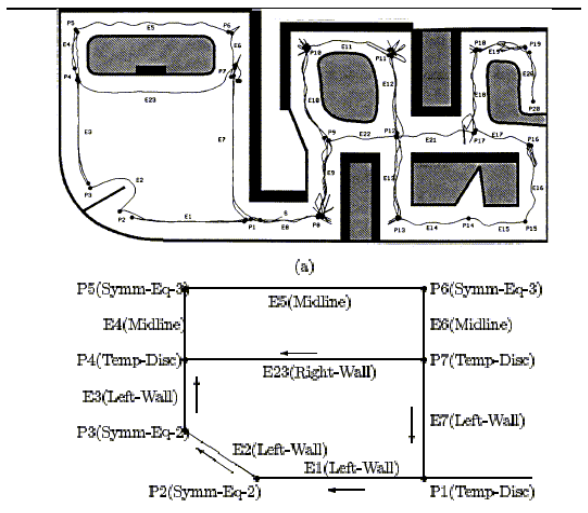
\includegraphics[width=0.5\textwidth]{topo_seman}\\
  \caption{Mapas topológico y semántico}\label{fg:semantico}
\end{figure}

De estos tres niveles, el más utilizado es, sin duda, el métrico. Su principal atractivo es la gran riqueza de su representación, lo que permite una navegación del robot más robusta. Los otros dos niveles de representación suelen construirse a partir del anterior y se utilizan para tareas de planificación de alto nivel. Su compacidad los hará interesantes en entornos estructuralmente complejos o de tamaño superior a los explorados hasta el momento.


 \subsection{SLAM con técnicas probabilísticas}
En cualquier modelo matemático de un sistema existen diversas fuentes de incertidumbre. En los sistemas dinámicos, además, puede haber perturbaciones que afecten al control. Por último, como ya se ha mencionado, los sensores no pueden suministrar información completa y exacta. Estas son algunas de las limitaciones por las que los modelos deterministas resultan insuficientes y por las que se llega al planteamiento de modelos estocásticos.

Desde los años 90 las principales técnicas de construcción de mapas y localización se han fundamentado en la teoría de la probabilidad y, más concretamente, en el teorema de Bayes. Los algoritmos que analizan la solución al problema SLAM desde esta perspectiva son claramente los que mejores resultados han tenido.
La formulación probabilística rigurosa del problema SLAM se conoce comúnmente como Filtro de Bayes y puede considerarse como una generalización temporal del teorema del mismo nombre. El planteamiento se expone a conti\-nuación\cite{Rodriguez-Losada04}.

En la construcción de un mapa por un robot móvil se tienen dos tipos de medidas: las que provienen de los sensores propioceptivos (odometría) y las de los sensores estereoceptivos (observaciones). Se puede suponer sin pérdida de generalidad que estas medidas llegan secuencial y alternativamente en el tiempo:

\begin{equation}\label{eq:medidas}
    u_{1},z_{1},u_{2},z_{2}...u_{t},z_{t}
\end{equation}

Donde $u$ representa un desplazamiento relativo del robot y $z$ una medida de los sensores externos. El subíndice indica el instante de tiempo al que corresponde cada medida, siendo $t$ el instante actual.
El estado del sistema en el instante $t$ típicamente vendrá dado por la posición del robot $s_{t}$ y la posición de los objetos del mapa $m_{t}$

\begin{equation}\label{eq:estado}
    x_{t}\sim s_{t},m_{t}
\end{equation}

El teorema de Bayes permite conocer la probabilidad de dicho estado condicionada a los datos recogidos hasta ese instante $t$. Hay que destacar que esta función de probabilidad representa cualquier solución probabilista al problema SLAM.

\begin{equation}\label{eq:prob_estado}
    p(x_{t}\mid z^{t},u^{t}) = p(s_{t},m_{t}\mid z^{t},u^{t})=\eta p(z_{t}\mid s_{t},m_{t},z^{t-1},u^{t})p(s_{t},m_{t}\mid z^{t-1}u^{t})
\end{equation}


\begin{eqnarray}
% \nonumber to remove numbering (before each equation)
    z^{t} = z_{1},z_{2}...z_{t} \nonumber\\
    u^{t} = u_{1},u_{2}...u_{t}
\end{eqnarray}

Aceptando que el único estado que existe es el definido por $s_{t}$ y $m_{t}$ (hipótesis de Markov), la función de probabilidad puede escribirse nuevamente:

\begin{equation}\label{eq:prob_markov}
    p(x_{t}\mid z^{t},u^{t}) = p(s_{t},m_{t}\mid z^{t},u^{t}) = \eta p(z_{t}\mid s_{t},m_{t})p(s_{t},m_{t}\mid z^{t-1}u^{t})
\end{equation}

El segundo factor puede expresarse en base al teorema de la probabilidad total como:
\begin{equation}\label{eq:prob_total}
    p(s_{t},m_{t}\mid z^{t-1},u^{t}) = \int\int p(s_{t},m_{t}\mid z^{t-1},u^{t},s_{t-1},m_{t-1})p(s_{t-1},m_{t-1}\mid z^{t-1},u^{t})ds_{t-1}dm_{t-1}
\end{equation}

Aplicando otra vez la hipótesis de Markov y el hecho de que es lógico pensar que el movimiento del robot es independiente del mapa, se tiene:

\begin{equation}\label{eq:termino2}
    p(s_{t},m_{t}\mid z^{t-1},u^{t}) = \int p(s_{t}\mid u_{t-1},s_{t-1})p(s_{t-1},m\mid z^{t-1},u^{t-1})ds_{t-1}
\end{equation}


Con lo que finalmente queda:
\begin{equation}\label{eq:filtroBayes}
  p(s_{t},m\mid z^{t},u^{t}) = \eta p(z_{t}\mid s_{t},m_{t})\int p(s_{t}\mid u_{t},s_{t-1})p(s_{t-1},m\mid z^{t-1},u^{t-1})ds_{t-1}
\end{equation}

Esta expresión \ref{eq:filtroBayes} es la que se conoce como Filtro de Bayes en el problema SLAM. El problema así planteado puede abordarse recursivamente si se conocen en cada instante las medidas sensoriales de ese instante (con su probabilidad) junto con la función de probabilidad del estado en el instante anterior.
Hacen falta, por lo tanto, dos funciones de probabilidad correspondientes a datos sensoriales: la relativa a la odometría, $p(s_{t}\mid u_{t},s_{t-1})$, y la de las medidas efectuadas por el sistema estereoceptivo, $p(z_{t}\mid s_{t},m_{t})$.

Sin embargo, la ecuación del Filtro de Bayes no puede resolverse ni implementarse directamente sino que es preciso realizar ciertas simplificaciones o suposiciones que dan lugar a los diferentes algoritmos existentes.

El estudio de todos estos algoritmos queda fuera del alcance de este proyecto ya que en él no se hace SLAM propiamente dicho, como se verá en el capítulo correspondiente. La solución adoptada se encuadra dentro de la categoría de métodos de Máxima Probabilidad Incremental. La idea básica del algoritmo así llamado consiste en construir un único mapa según van llegando los datos, sin mantener ninguna noción sobre la incertidumbre del mismo o de la posición del robot en cada instante. Únicamente se determinan la posición y el mapa más probables en cada momento. La principal ventaja del algoritmo es su mayor simplicidad y el menor tiempo de procesamiento y capacidad de almacenamiento que requiere frente a otras soluciones. Sin embargo, no presenta un buen comportamiento a la hora de cerrar bucles dado que al no guardarse ninguna información sobre la incertidumbre del mapa, una estimación realizada no puede corregirse a partir de datos posteriores. Una posible forma de hacer frente a este problema es utilizar algoritmos híbridos. Los algoritmos híbridos ofrecen una aproximación intermedia entre la obtención del mapa más probable sin mantener una noción de la incertidumbre del mismo ni de la posición del robot (algoritmo de Máxima Probabilidad Incremental), y la estimación de la función de probabilidad del mapa completo (solución SLAM-EKF), que conserva la totalidad de la información sobre la incertidumbre. En definitiva lo que hacen este tipo de algoritmos es mantener la incertidumbre en la posición del robot de una u otra forma y estimar el mapa más probable simplificando la ecuación \ref{eq:filtroBayes} para la localización en un mapa dado.


%El sistema de localización implementado no incorpora la construcción simultánea de mapas de los tipos descritos en el capítulo de estado del arte sino que elabora y luego va actualizando un mapa de puntos a partir de las observaciones correspondientes a las medidas del láser. Son los puntos que ya forman parte del mapa los que se utilizan para la localización en cada instante.

\subsection {Localización probabilística basada en mapas}

Entre las técnicas probabilistas de localización destacan especialmente dos tipos de localización: \emph{localización de Markov} y \emph{localización basada en el filtro de Kalman}. El primero de ambos métodos utiliza una distribución de probabilidad explícitamente especificada sobre todas las posibles posiciones del robot en el mapa. No requiere que el robot tenga una posición inicial conocida y permite la relocalización a partir de situaciones ambiguas. Sin embargo, para actualizar la probabilidad de todas las posiciones del espacio de estado hace falta que éste tenga una representación discretizada (mapas de celdillas, mapas topológicos\ldots).

En 1994 se celebró el concurso \emph{1994 American Association for Artificial Intelligence (AAAI) National Robot Contest}, en el que se proporcionaba a los robots participantes un mapa topológico imperfecto del entorno con el cual tenían que conseguir llegar a una determinada habitación establecida como meta. El robot Rinho empleaba en dicho concurso localización de Markov a partir de la construcción de un mapa de celdillas. En la figura \ref{fg:MarkovGrid} pueden verse sus resultados.

\begin{figure}[h]
  % Requires \usepackage{graphicx}
  \centering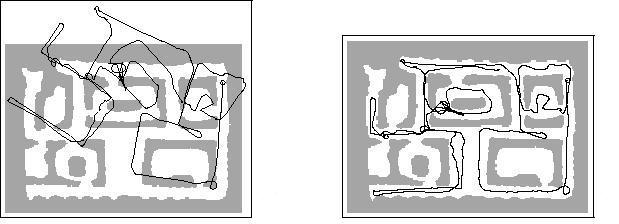
\includegraphics[scale=0.8]{Markov}\\
  \caption{ Trayectorias odométrica y corregida mediante localización de Markov en un mapa de ocupación de celdillas \cite{Fox99}}\label{fg:MarkovGrid}
\end{figure}

Las técnicas de localización de Markov con mapas topológicos son difíciles de aplicar en entornos no estructurados. En otro tipo de casos, sin embargo, puede ser más adecuado. El ganador de la competición de robots móviles de la AAAI de 1994, llamado Dervish, empleaba localización probabilística de Markov sobre representación topológica del entorno. En la figura \ref{fg:MarkovTop} se muestra un ejemplo de representación topológica de un entorno de oficinas similar al del concurso. Dervish detectaba las puertas cerradas y las puertas abiertas, guardando la información para relacionarla con la conectividad de nodos del mapa. Posteriores desarrollos pueden encontrarse en \cite{Simmons95} y \cite{Kaebling96}.

\begin{figure}[h]
  % Requires \usepackage{graphicx}
  \centering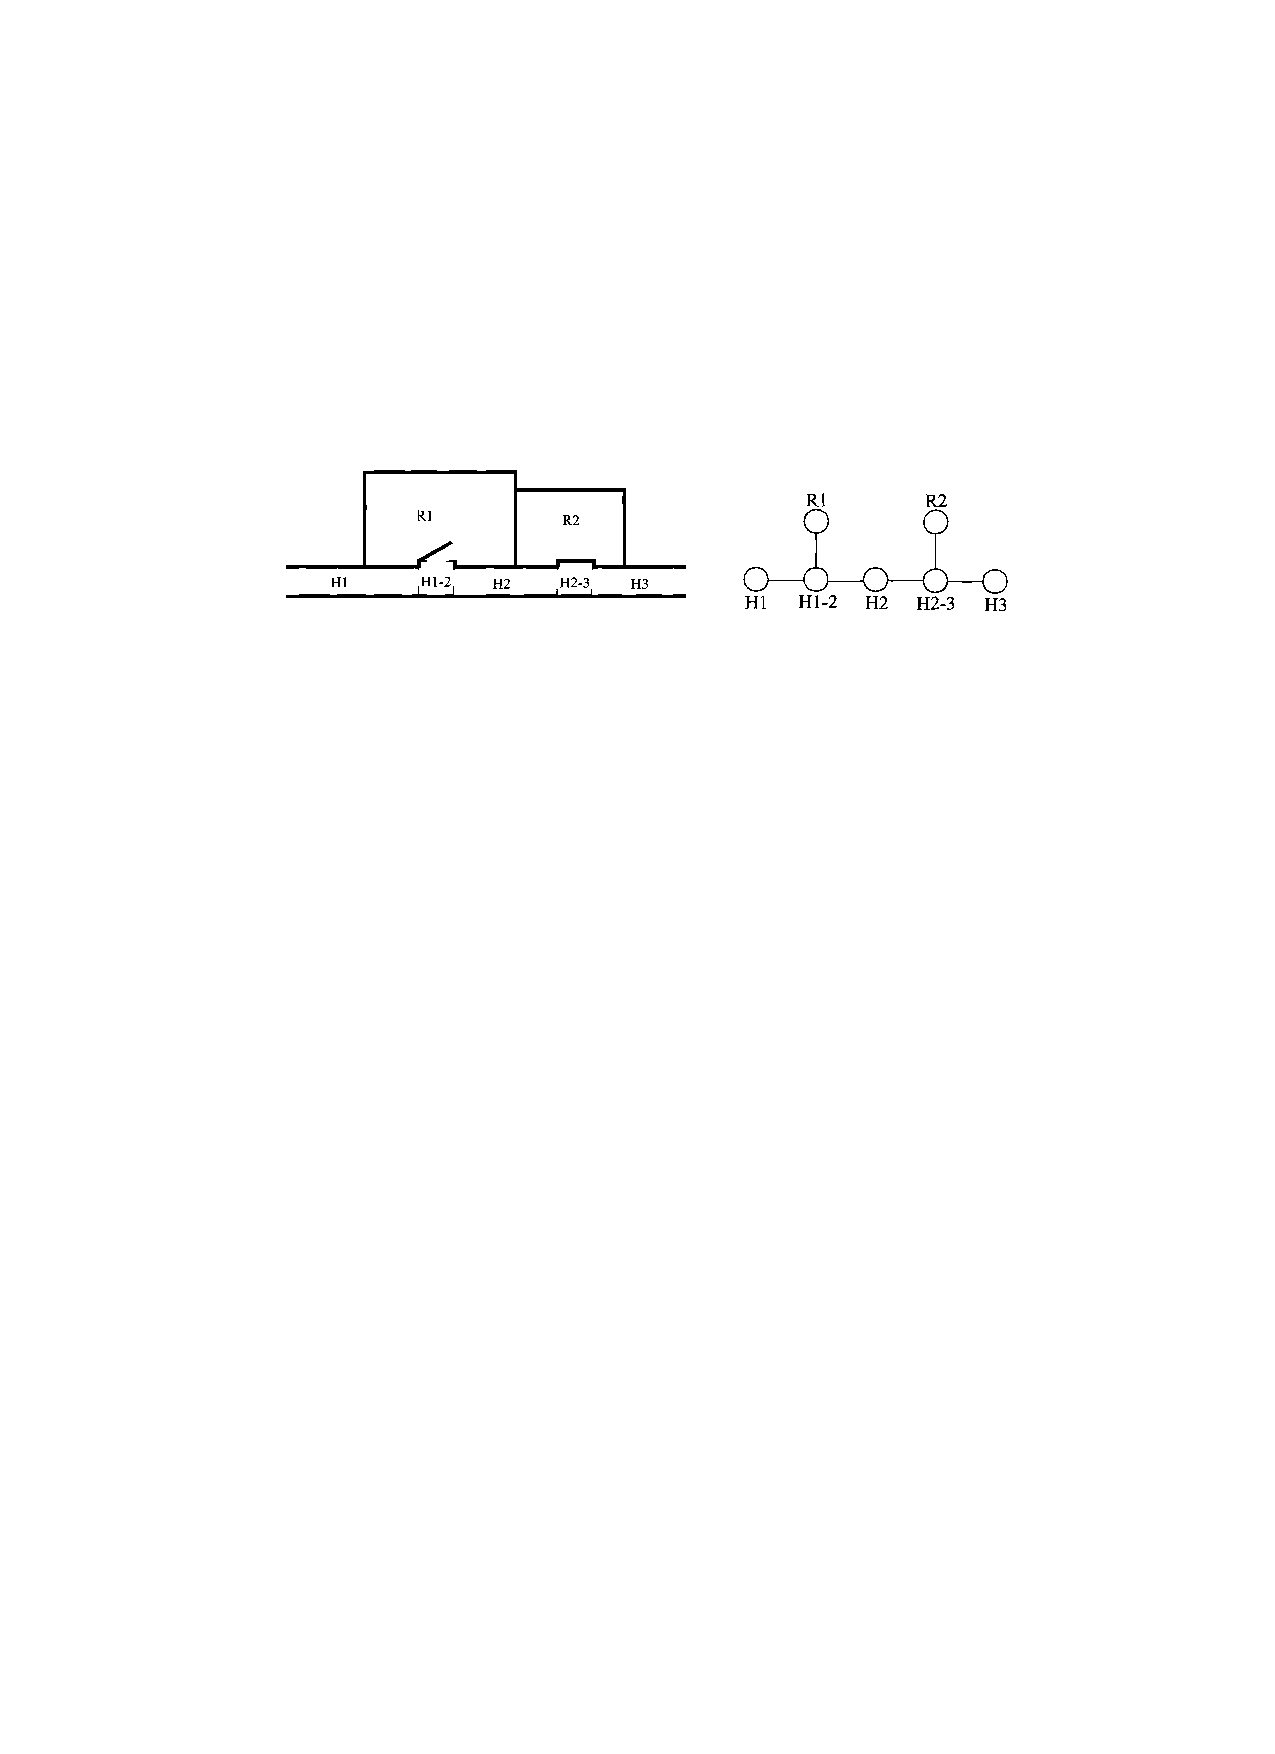
\includegraphics[scale=0.8]{TopoOffice}\\
  \caption{Representación topológica de un entorno de oficina}\label{fg:MarkovTop}
\end{figure}


Otro tipo de localización basada en el método de Markov es la \emph{ localización de Monte Carlo}. En ella, inicialmente se toma al azar  un elevado número de posibles configuraciones hipotéticas para el robot. Con las medidas de los sensores se va actualizando la probabilidad de que cada una de esas configuraciones sea la configuración del robot en ese instante en base a modelos estadísticos mediante aplicación del teorema de Bayes. De un modo similar, cada movimiento incremental del robot se incorpora al cálculo de probabilidades mediante el modelo estadístico de la medida del movimiento. Las configuraciones cuya probabilidad resulta ser muy baja se sustituyen por otras configuraciones aleatorias del espacio de estado.

El filtro de Kalman emplea una representación de densidad de probabilidad Gaussiana de la posición del robot y la asociación de datos para la localización. Es interesante el hecho de que el proceso de localización del filtro de Kalman es el resultante si se aplica al modelo de Markov la suposición de que la incertidumbre en la posición del robot sigue una distribución normal.

Las principales ventajas de la localización mediante filtro de Kalman son su precisión y eficiencia cuando se conoce la posición de partida en el movimiento del robot, el poder aplicarse con modelos de representación del entorno continuos (mapas geométricos) y las menores necesidades de tiempo y memoria respecto a la localización de Markov. El mayor inconveniente que presenta es la posibilidad de que el robot quede completamente perdido si el error en su movimiento es demasiado grande (como resultado del choque con un obstáculo, por ejemplo).

\subsection {Filtro de Kalman}
La localización basada en el filtro de Kalman es la más extendido en la literatura y en implementaciones prácticas y debido a sus buenas propiedades, apropiadas para la mayor parte de aplicaciones, es la que se ha utilizado en el desarrollo de este proyecto.

\subsubsection {Conceptos introductorios}
El filtro de Kalman es un algoritmo recursivo óptimo para procesar información\cite{Maybeck79}. Combina la totalidad de la información disponible, ponderándola según su grado de incertidumbre, para realizar la estimación de las variables que definan el estado del sistema. El funcionamiento del filtro requiere el conocimiento de la dinámica del sistema, así como de los modelos estadísticos del ruido en las medidas de los sensores y de la incertidumbre inicial del modelo del sistema. Al tratarse de un algoritmo recursivo, cada estimación se efectúa a partir de la anterior y de la nueva información disponible, sin que sea preciso almacenar todos los datos previos.

El filtro de Kalman permite minimizar el error en la estimación de las variables de interés cuando el modelo es lineal y la incertidumbre del sistema y de las medidas de los sensores es ruido blanco gaussiano. En esta situación, la función de densidad de probabilidad de cada variable a analizar condicionada a las medidas tomadas es tal que la media, la moda y la mediana coinciden, lo que evita cualquier posible conflicto a la hora de determinar cuál es la mejor estimación.
Las hipótesis aceptadas pueden parecer altamente restrictivas pero hacen posible la resolución matemática del problema y se acercan bastante bien a la realidad en la mayoría de los casos. En otros, sin embargo, han de contemplarse algunas variaciones y resulta de utilidad el llamado filtro extendido de Kalman (EKF).

\subsubsection{Ecuaciones para sistemas dinámicos}
A continuación se muestran las ecuaciones que definen el comportamiento del filtro de Kalman aplicado a sistemas dinámicos\cite{Schutter99}.

La relación entre cada una de las medidas tomadas en un instante y el estado del sistema es del tipo:
\begin{equation}\label{eq:measurement}
   z_{k} = H_{k}x_{k}+\rho_{m}
\end{equation}
Con z vector de medidas, x vector de estado y $\rho_{m}$ ruido gaussiano en las medidas, con media nula y matriz de covarianza $R_{k}$ ó $R$ si ésta es constante en el tiempo.

Se considera que la evolución del sistema sigue el siguiente modelo de estado lineal:
\begin{equation}\label{eq:model}
    x_{k} = Ax_{k-1}+Bu_{k-1}+\rho_{\rho},
\end{equation}
donde A es la matriz de estado; B, la matriz de entrada; $u_{k-1}$, el vector de entrada en el instante k-1 y $\rho_{\rho}$ representa la incertidumbre del proceso (con matriz de covarianza $Q_{p}$, o $Q_{p_{k-1}}$ si es variable con el tiempo).


\textbf{Etapa de predicción}
Así, la \emph{predicción del estado}, $\tilde{x}_{k}$, vendrá dada por:
\begin{equation}\label{eq:x_prediction}
    \tilde{x}_{k} = A\hat{x}_{k-1}+Bu_{k-1},
\end{equation}

siendo $\hat{x}_{k-1}$ la estimación del estado en el instante k-1.

Si la entrada $u$ se conoce con exactitud, el error de predicción dado por la diferencia entre \ref{eq:x_prediction} y \ref{eq:model} será:
\begin{equation}\label{eq:prediction_error}
    \tilde{x}_{k}-x_{k} = A(\hat{x}_{k-1}-x_{k-1})- \rho_{\rho}
\end{equation}

y la matriz de covarianza de $x_{k}$ queda:
\begin{equation}\label{eq:P_prediction}
    \tilde{P}_{k} = A\hat{P}_{k-1}A^{T}+Q_{p_{k-1}}
\end{equation}


\textbf{Etapa de corrección}
La solución de mínimos cuadrados entre las medidas y las medidas esperadas es:
\begin{equation}\label{eq:x_estimation}
    \hat{x}_{k} = \tilde{x}_{k}+K_{k}(z_{k}-H_{k}\tilde{x}_{k})
\end{equation}

\begin{equation}\label{eq:P_estimation}
    \hat{P}_{k} = (I-K_{k}H_{k})\tilde{P}_{k}
\end{equation}

con
\begin{equation}\label{eq:K}
    K_{k} = \tilde{P}_{k}H_{k}^{T}S_{k}^{-1}
\end{equation}

\begin{equation}\label{eq:S}
    S_{k} = R_{k}+H_{k}\tilde{P}_{k}H_{k}^{T}
\end{equation}

Estas ecuaciones constituyen el llamado filtro \emph{dinámico} de Kalman.
La matriz $K_{k}$ se denomina \emph{ganancia de Kalman}.
La diferencia entre las medidas en k y sus valores esperados, $v_{k} = z_{k}-H_{k}\tilde{x}_{k}$, se conoce como la \emph{innovación} del proceso y la matriz $S$ corresponde a su matriz de covarianza.

El filtro de Kalman \emph{estático} es un caso particular del anterior y se obtiene a partir de estas ecuaciones haciendo $A = I$, $B = 0$ y $Q_{p} = 0$.

\subsection{Filtro Extendido de Kalman}
La principal aportación de este algoritmo respecto al del filtro de Kalman convencional es su extensión a sistemas no lineales. También permite incorporar los casos en los que la relación entre el estado y las medidas de los sensores externos no puede definirse de forma explícita. La convergencia del EKF depende de diversos factores como pueden ser la estimación inicial, las no linealidades de las ecuaciones, el orden en que se procesan las medidas...De este modo, no existe prueba formal de la convergencia del algoritmo, sino tan solo ciertos tests de consistencia que evalúan el comportamiento del mismo en cada caso.

\subsubsection{Ecuaciones para sistemas no lineales}
Las ecuaciones del medida \ref{eq:measurement} y de estado \ref{eq:model}, frecuentemente presentan carácter no lineal:
\begin{equation}\label{eq:medida_nolineal}
    z = h(x)+\rho_{m}
\end{equation}

\begin{equation}\label{eq:estado_nolineal}
    x_{k} = f(x_{k-1},u_{k-1})+\rho_{\rho},
\end{equation}

cuyas ecuaciones linealizadas en la estimación más reciente son:
\begin{equation}\label{eq:medida_linealizada}
    z = h(\tilde{x}_{k})+\frac{\delta h}{\delta x}|_{ _{\tilde{x}_k}} (x-\tilde{x}_{k})+\rho_{m}
\end{equation}

\begin{equation}\label{eq:estado_linealizada}
    x_{k} = f(\hat{x}_{k-1},u_{k-1})+\frac{\delta f}{\delta x}\mid _{_{\hat{x}_k-1}} (x_{k-1}-\hat{x}_{k-1})+\rho_{\rho}
\end{equation}

Con ello, las ecuaciones del EKF se obtienen de la siguiente manera:


\textbf{Etapa de predicción}
\begin{equation}\label{eq:x_predictionEKF}
    \tilde{x}_{k} = f(\hat{x}_{k-1},u_{k-1})
\end{equation}

Sustituyendo $A$ por $\frac{\delta f}{\delta x}\mid _{\hat{x}_k-1}$ en \ref{eq:P_prediction}:
\begin{equation}\label{eq:P_predictionEKF}
    \tilde{P}_{k} = (\frac{\delta f}{\delta x}\mid_{ _{\hat{x}_k-1}}) \hat{P}_{k-1} (\frac{\delta f}{\delta x}\mid_{ _{\hat{x}_k-1}})^{^{T}}+Q_{p_{k-1}}
\end{equation}


\textbf{Etapa de corrección}
Empleando la ecuación de medida no lineal para realizar la predicción de las medidas, \ref{eq:x_estimation} pasa a ser:
\begin{equation}\label{eq:x_estimationEKF}
    \hat{x}_{k} = \tilde{x}_{k}+K_{k}(z_{k}-h(\tilde{x}_{k})),
\end{equation}
donde se aprecia que la innovación es, en este caso, $v_{k} = z_{k}-h(\tilde{x}_{k})$.

Para completar el algoritmo,  \ref{eq:P_estimation}, \ref{eq:K}, \ref{eq:S} se modifican mediante $H_{k}\leftarrow \frac{\delta h}{\delta x}\mid_{\hat{x}_{k-1}}$:

\begin{equation}\label{eq:P_estimationEKF}
    \hat{P}_{k} = (I-K_{k}\frac{\delta h}{\delta x}\mid _{_{\hat{x}_{k-1}}})\tilde{P}_{k}
\end{equation}

\begin{equation}\label{eq:KEKF}
    K_{k} = \tilde{P}_{k}(\frac{\delta h}{\delta x}\mid _{_{\hat{x}_{k-1}}})^{T}S_{k}^{-1}
\end{equation}

\begin{equation}\label{eq:SEKF}
    S_{k} = R_{k}+(\frac{\delta h}{\delta x}\mid _{\hat{x}_{k-1}})\tilde{P}_{k} (\frac{\delta h}{\delta x}\mid _{_{\hat{x}_{k-1}}})^{T}
\end{equation}

\subsubsection{Ecuaciones para el caso de ecuación de medida en forma implícita}

No siempre es posible despejar $z$ en la forma de \ref{eq:measurement}. En su lugar, a veces sólo se dispone de ecuaciones implícitas del tipo:
\begin{equation}\label{eq:implicit}
    h(x,z)+\rho_{m}=c,
\end{equation}
con c vector de constantes.
En este caso, las ecuaciones anteriores varían del siguiente modo:


\textbf{Etapa de predicción}
No se ve afectada, ya que en ella no influyen las medidas estereoceptivas.


\textbf{Etapa de corrección}
Al ser ahora la innovación $v_{k}=c-h(\tilde{x}_{k},z_{k})$, la ecuación \ref{eq:x_estimationEKF} se transforma en:
\begin{equation}\label{eq:x_estimationIm}
    \hat{x}_{k} = \tilde{x}_{k}+K_{k}(c-h(\tilde{x}_{k},z_{k}))
\end{equation}

En las expresiones \ref{eq:P_estimation}, \ref{eq:K}, \ref{eq:S} ha de efectuarse el cambio $H_{k}\leftarrow \frac{\delta h}{\delta x}\mid_{\tilde{x}_{k},z_{k}}$. La matriz $R_{k}$ ha de sustituirse por $(\frac{\delta h}{\delta z} \mid _{\tilde{x}_{k},z_{k}}) R_{k} (\frac{\delta h}{\delta z} \mid _{\tilde{x}_{k},z_{k}})^{T}$.

 \begin{equation}\label{eq:P_estimationEKF_im}
    \hat{P}_{k} = (I-K_{k}\frac{\delta h}{\delta x}\mid_{\tilde{x}_{k},z_{k}})\tilde{P}_{k}
\end{equation}

\begin{equation}\label{eq:KEKF_im}
    K_{k} = \tilde{P}_{k}(\frac{\delta h}{\delta x}\mid_{\tilde{x}_{k},z_{k}})^{T}S_{k}^{-1}
\end{equation}

\begin{equation}\label{eq:SEKF_im}
    S_{k} = (\frac{\delta h}{\delta z} \mid _{\tilde{x}_{k},z_{k}}) R_{k} (\frac{\delta h}{\delta z} \mid _{\tilde{x}_{k},z_{k}})^{T}+(\frac{\delta h}{\delta x}\mid_{\tilde{x}_{k},z_{k}})\tilde{P}_{k} (\frac{\delta h}{\delta x}\mid_{\tilde{x}_{k},z_{k}})^{T}
\end{equation}

Una forma de comprobar que una innovación es consistente con el modelo consiste en calcular la llamada distancia de Mahalanobis de la misma y determinar si este valor de la adecuación de la medida al estado se encuentra dentro del intervalo de confianza escogido. El cuadrado de la distancia de Mahalanobis se calcula mediante $v_{k}^{T}S_{k}^{-1}v_{k}$ y también recibe el nombre de \emph{Normalised Innovation Squared}, $NIS_{k}$. Este parámetro tiene distribución $\chi^{2}$ con tantos grados de libertad como medidas independientes haya en el vector de medidas $z_{k}$, con lo que la decisión de aceptar o rechazar la medida se hará en base a:
\begin{equation}\label{eq:mahalanobis}
    v_{k}^{T}S_{k}^{-1}v_{k}<\chi^{2}_{dim(v_{k}),\alpha = confianza}
\end{equation}



\part{Desarrollo}
% -*- coding: utf-8 -*-

\chapter{Arquitectura del sistema}

\section{Plataformas de desarrollo y ejecución}

En la realización de este proyecto se ha utilizado una estación de trabajo PC con una configuración de software acorde con las prácticas habituales del grupo de robótica móvil:

\begin{itemize}
  \item Sistema Operativo Windows XP$^{®}$
  \item Lenguaje de programación C++ sobre el entorno de desarrollo MS Visual C++ 6.0$^{®}$ y posteriormente sobre Visual Studio .NET 2005$^{®}$ (Visual Studio 8).
\end{itemize}

Con ello se consigue la compatibilidad con otros trabajos del grupo y se tiene una buena portabilidad del desarrollo. También se ha comprobado que el paso al sistema operativo Windows Vista$^{®}$ es directo y no plantea ningún tipo de problema.

Algunas de las ventajas del lenguaje C++ son su buena capacidad de cálculo, el hecho de que es un lenguaje orientado a objetos y que se trata de un lenguaje de alto nivel con flexibilidad y potencia expresiva. Todo ello permite reducir el tamaño y la complejidad del código. Además, al tratarse de un lenguaje compilado, presenta una buena eficiencia en tiempos de ejecución frente a los lenguajes interpretados. También cabe destacar que gran parte de los entornos de programación distribuidos por los fabricantes de robots móviles están escritos en este lenguaje. Por supuesto, también es compatible con plataformas de desarrollo libre (como la herramienta Player/Stage/Gazebo, que proporciona software gratuito para el desarrollo de aplicaciones con robots y sensores sin imponer un lenguaje de programación determinado).

Respecto al sistema operativo, el uso de Visual Studio impone utilizar Windows. Este entorno simplifica la creación y compilación de código y, sobre todo, permite el tratamiento de cuadros de diálogo e interfaces gráficas para aplicaciones Windows de un modo sencillo. No obstante, son muy abundantes los trabajos en robótica móvil desarrollados con Linux$^{®}$ (Player \& Stage, por ejemplo, no se puede emplear en Windows).

Se han realizado versiones iniciales en modo consola (sobre todo cuando se empleaba simultáneamente el simulador \emph{MobileSim} del robot Pioneer) y finalmente se ha optado por aplicaciones de tipo MFC (ver \ref{mfc} basadas en cuadros de diálogo.

El modo de operación puede ser de tipo \emph{simulación}, \emph{fichero} o \emph{real}. La simulación permite observar en pantalla el movimiento teórico de un robot ficticio ante instrucciones que se le dan por medio del ratón o del teclado. Con el modo fichero se muestra de forma similar el comportamiento del sistema al utilizar unos datos de odometría y de medidas del láser guardados previamente en un fichero. El modo real es el que se emplea con el robot verdadero y también permite visualizar los resultados sobre la interfaz gráfica.

Respecto a la plataforma de ejecución para el modo real, en diferentes fases del ciclo de vida del proyecto se han utilizado los robots Pioneer y Urbano. A este último corresponde la implementado el sistema completo y con él se ha llevado a cabo la mayor parte de las pruebas.

En el caso del Pioneer P3AT, la puesta en funcionamiento se ha basado en comunicación con cable serie entre un computador portátil y el robot.

Como se ha visto en la introducción, el computador base de Urbano es un PC Pentium con sistema operativo GNU/Linux. También cuenta con un computador secundario que es un PC Pentium con Windows XP. La conexión entre la plataforma de desarrollo y el robot se realiza con un ordenador portátil mediante conexión \emph{telnet} a través de cable Ethernet.

\section{Bibliotecas empleadas}
Para el desarrollo del software del proyecto se ha hecho uso de varias bibliotecas existentes.

\subsection{Standard Template Library (STL)}

Biblioteca de C++ que incluye clases contenedoras, algoritmos e iteradores. Las clases contenedoras son patrones (\emph{templates}) que permiten almacenar objetos de tipos muy variados. Los iteradores son una generalización de los punteros y sirven para acceder a los elementos almacenados en los contenedores. Así, se dice que la STL es una biblioteca \emph{genérica}, ya que sus componentes están altamente parametrizados.

La STL incluye un gran número de algoritmos para manipular los datos guardados en los contenedores. Las funciones que implementan estos algoritmos deberán tomar como argumentos tipos de datos coherentes con las operaciones a realizar. El conjunto de requisitos que debe tener un tipo de dato recibe el nombre de \emph{concepto}. En la STL se definen los siguientes conceptos para clasificar los iteradores: \prog{OutputIterator}, \prog{InputIterator}, \prog{ForwardIterator}, \prog{Bidireccional-} \prog{Iterator}, \prog{RandomAccessIterator}. Algunos de ellos son \emph{refinamientos} de otros, lo que implica una relación similar a la herencia en la programación orientada a objetos.

La clase \prog{vector} es una clase contenedora de tipo secuencial y, como cualquier \emph{template}, puede ser particularizada para contener diferentes tipos de objetos. Se trata de una extensión de los vectores o \emph{arrays} disponibles en C++, con la ventaja de que el número de elementos almacenados puede variar dinámicamente, realizándose la gestión de memoria de forma automática.
Esta clase ha sido ampliamente utilizada en el proyecto.

\subsection{Microsoft Foundation Class Library (MFC)} \label{mfc}

La biblioteca de clases base de Microsoft encapsula gran parte de la API de Windows en clases de C++. Constituye una importante herramienta para desarrollar aplicaciones Windows con entornos de ventanas, menús, etc. Proporciona, entre otras cosas, un gran número de clases para manejar distintos tipos de ventanas predefinidas y para incluir los controles más comunes en cuadros de diálogo.

En el tipo de proyecto empleado se crea una interfaz gráfica constituida por un cuadro de diálogo principal que hereda de la clase pública \prog{CDialog}. Un editor de recursos disponible en Visual Studio facilita la forma de añadir botones al mismo y la declaración de funciones asociadas a los diferentes eventos que pueden tener lugar sobre ellos.

\subsection{Open Graphics Library (OpenGL)}

Biblioteca de funciones estándar para el dibujo de gráficos 2D y 3D. Permite variar los colores, el tamaño y la posición de los objetos, el grosor de las líneas, los focos de luz, los puntos de vista, etc.

En este proyecto se ha utilizado la clase \prog{COpenGLWnd}, implementada por Diego Rodríguez-Losada, como clase base de una nueva clase llamada \prog{CRobotMo-} \prog{veGLWnd}. \prog{COpenGLWnd} hereda de la clase \prog{CWnd} de las MFC y permite crear una ventana con fondo negro sobre el que se dibuja una cuadrícula de color magenta y los ejes de un sistema de referencia global para el movimiento sobre un plano. También incluye diversas funcionalidades para cambiar el punto de vista por medio del ratón o el teclado y sirve para dibujar diferentes tipos de robots. En la clase \prog{CRobotMoveGLWnd} se maneja el dibujo de trayectorias, obstáculos, puntos del mapa, polígonos\ldots Se ha reprogramado la función virtual \prog{OnKeyDown} de la clase \prog{COpenGLWnd} para modificar las opciones de visualización desde el teclado y para hacer funcionar al robot en modo teleoperado. Desde ella se realiza también el desplazamiento del dibujo del robot de acuerdo con el movimiento del mismo.

\subsection{Biblioteca Mathematics}
Biblioteca desarrollada por Diego Rodríguez-Losada para facilitar el tratamiento de la geometría y distintos tipos de operaciones. En el proyecto se utiliza principalmente para la definición de puntos y segmentos (clases \prog{Point2D} y \prog{Segment2D}). También se dispone de los ficheros \prog{maths.h}, \prog{maths.cpp}, \prog{matrix.h},  \prog{matrix.cpp}, del mismo autor, para definir matrices y operar con ellas.

%Algunas de sus funciones, no obstante, habían sido previamente implementadas en el fichero \prog{tools.cpp}.

\subsection{Biblioteca Aria}

Aria (Advanced Robot Interface for Applications) es una interfaz para el uso de los robots de la firma MobileRobots.Inc que puede usarse sobre las APIs de Linux y Win32. Integra software para establecer las comunicaciones, para controlar la velocidad y la orientación de los robots, para la utilización de diferentes sensores y accesorios\ldots Se trata de una biblioteca escrita en C++, pero también puede ser ampliamente utilizada en Java o Phyton mediante \emph{wrappers}.

En el proyecto se han utilizado únicamente las funciones básicas que permiten la conexión y desconexión sencilla del robot, el envío de comandos de movimiento de bajo nivel (velocidades de avance y giro) y la lectura de los datos proporcionados por los encóders. La mayor parte de estas funciones se encapsulan dentro de la clases \prog{ArRobot} y \prog{ArSimpleConnector}.

El equivalente a las funciones indicadas ha sido implementado en la clase \prog{CPioneer} para no tener dependencias de Aria fuera de dicha clase.
Además, se utilizan como variables miembro punteros a void, que primeramente se inicializan a NULL para después hacer un cast a vectores que apuntan a los objetos correspondientes (\prog{ArRobot}, \prog{ArSimpleConnector}). Con esto se evita que al ejecutarse la aplicación sea necesario tener instalado el software de Aria.

\section{Funciones auxiliares utilizadas}
A lo largo del desarrollo del proyecto se han creado algunas funciones de carácter auxiliar para realizar ciertas operaciones. Su declaración y contenido se pueden encontrar en los ficheros \prog{tools.h} y \prog{tools.cpp} Las más destacadas son:

\begin{itemize}
  \item \prog{AngRango}: se emplea para convertir un ángulo dado en su equivalente dentro del intervalo [-PI, PI]
  \item \prog{ErrAng}: sirve para calcular el ángulo perteneciente a [-PI, PI] que separa un ángulo de partida de un ángulo de destino por el camino más corto
  \item \prog{Comp}: se utiliza para realizar la composición de dos transformaciones relativas (Ver Anexo A)
  \item \prog{J1}: sirve para calcular la matriz jacobiana de una composición de dos transformaciones relativas respecto de la primera variable (Ver Anexo A)
  \item \prog{J2}: se emplea para obtener la matriz jacobiana de una composición de dos transformaciones relativas respecto de la segunda variable (Ver Anexo A)
  \item \prog{eye}: sirve para crear una matiz identidad de las dimensiones que queramos
  \item \prog{InvTrans}: permite calcular la inversión de una transformación relativa entre dos sistemas de referencia (Ver Anexo A)
\end{itemize}

Las dos primeras funciones resultan de utilidad en el control, la planificación de trayectorias y el control reactivo. El resto se utilizan principalmente para la localización y en el tratamiento de los mapas.

\section{ Estructura de clases}
En la figura \ref{fg:uml} se puede ver el diagrama UML de las clases que conforman el sistema.

\begin{figure}[h]
  % Requires \usepackage{graphicx}
  \centering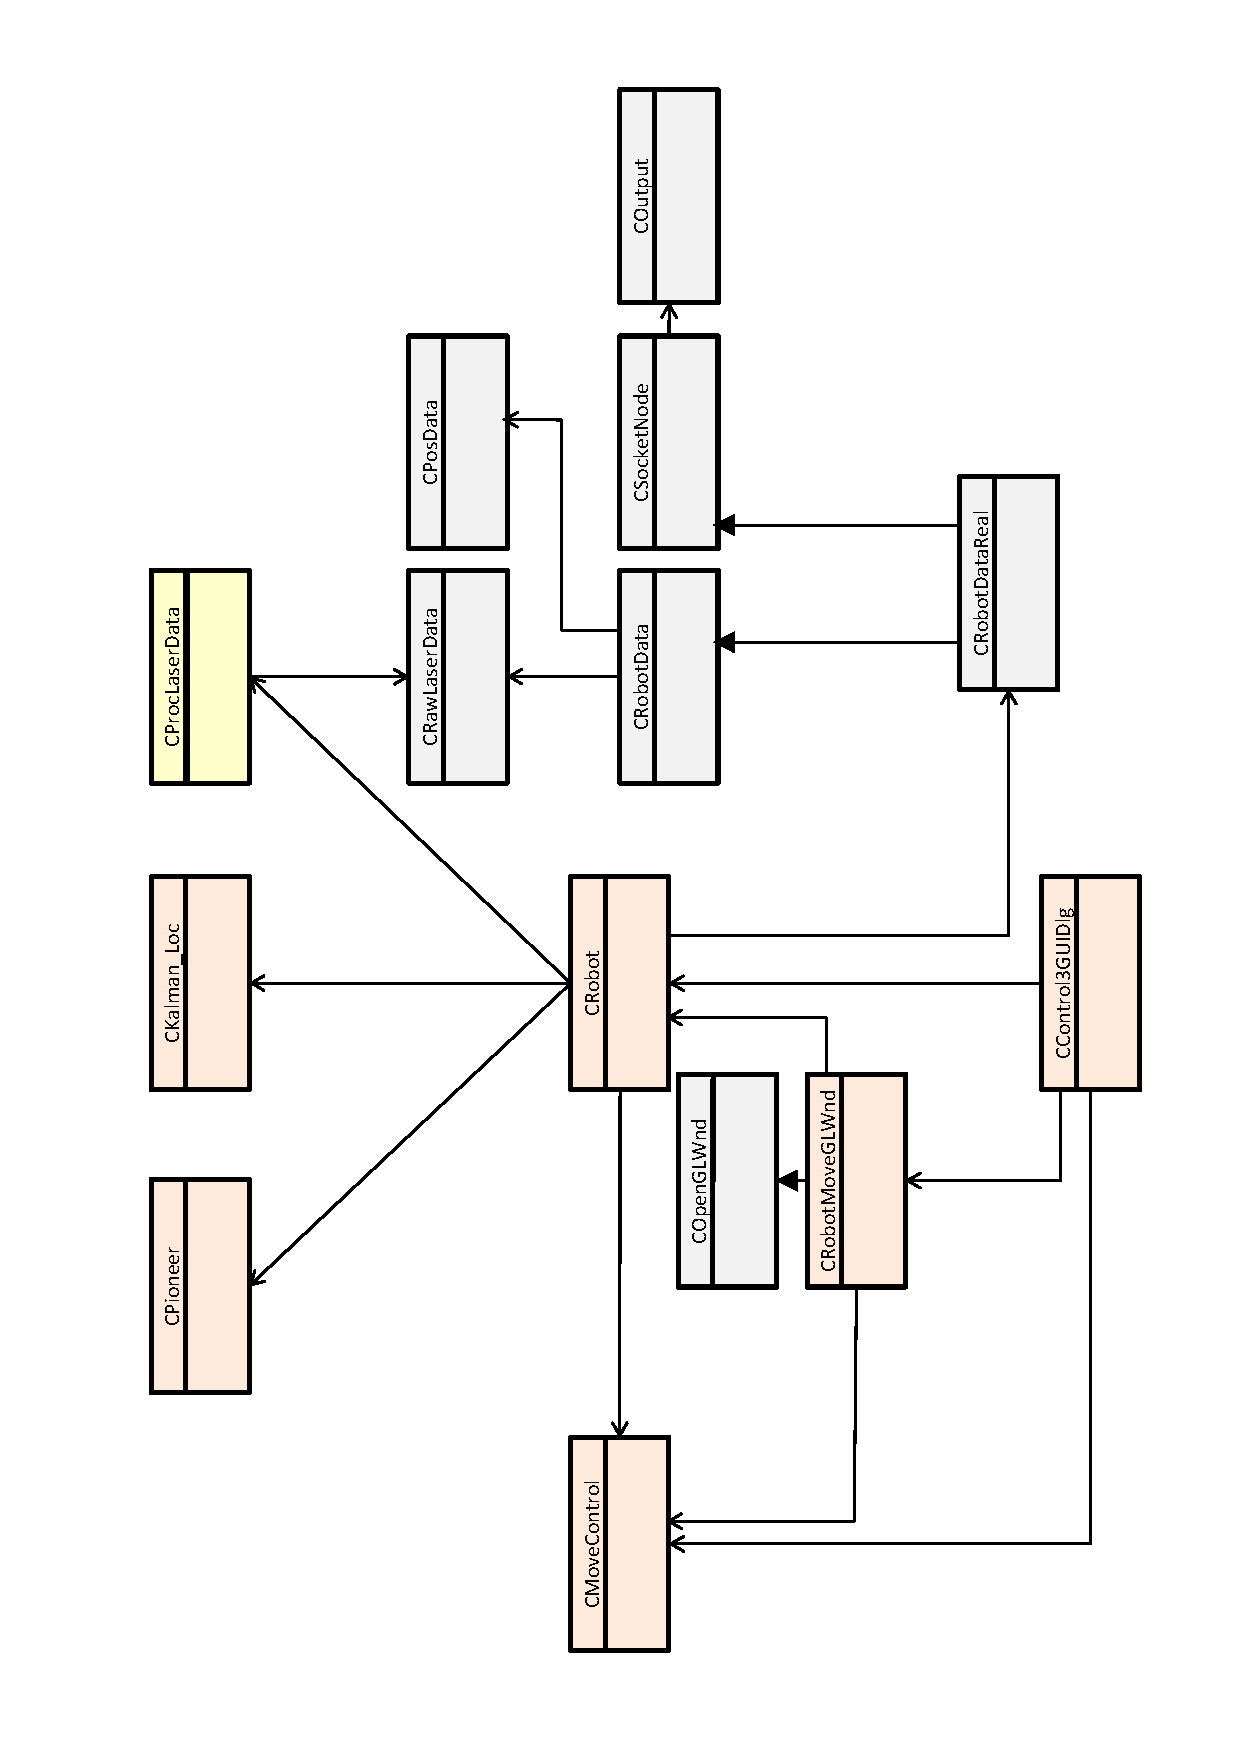
\includegraphics[scale=0.7]{clases4}\\
  \caption{Diagrama de clases del sistema}\label{fg:uml}
\end{figure}

En el diagrama no se muestran las dependencias de las bibliotecas anteriormente descritas. Las clases que han sido implementadas en el presente proyecto aparecen en color rosa. El color gris se ha utilizado para las clases que existían previamente. La clase \prog{CProcLaserData} forma parte de este último grupo, pero ha sido ligeramente modificada.

A continuación se explica el uso que se ha hecho de estas clases mientras que las clases nuevas serán tratadas en posteriores capítulos, después de que se estudien los algoritmos incorporados.

\clearpage

\subsection{La clase \prog{CRawLaserData}}
Esta clase se encarga principalmente de leer y escribir ficheros con los datos procedentes del láser y de ajustar dicha información al formato correspondiente para ser enviada o tras ser recibida por un socket. También define una macro con el máximo número de medidas que puede proporcionar el láser, 361.
Sus métodos son los siguientes:

\subsubsection{Load}

\noindent
\prog{int Load(FILE* source\_file)}

\noindent
Esta función se emplea para leer de un fichero los datos correspondientes a las medidas del láser.

\begin{itemize}
  \item \prog{source_file}: fichero del que se lee la información del láser
\end{itemize}

\noindent
Los resultados obtenidos sobre el instante en que se efectúa la medida, el identificador del láser, el número de medidas, el ángulo recorrido por éste y su resolución y el máximo alcance del láser se almacenan en variables con nombres representativos: \prog{time_stamp\_seconds}, \prog{time_stamp_useconds}, \prog{id_laser}, \prog{num_med}, \prog{scan_angle}, \prog{scan_resolution}, \prog{max_range}\ldots

Estos datos han de ir seguidos de dos puntos, :, y detrás han de aparecer las medidas sucesivas de las distancias asociadas a cada ángulo, que se van guardando en el vector de enteros \prog{med}. Todos los valores deben ir separados por un espacio en blanco para ser leídos correctamente. En el ejemplo de la figura \ref{fg:ficherolaser} puede verse mejor cómo ha de ser el formato de una línea del fichero:

\begin{figure}[h]
  % Requires \usepackage{graphicx}
  \centering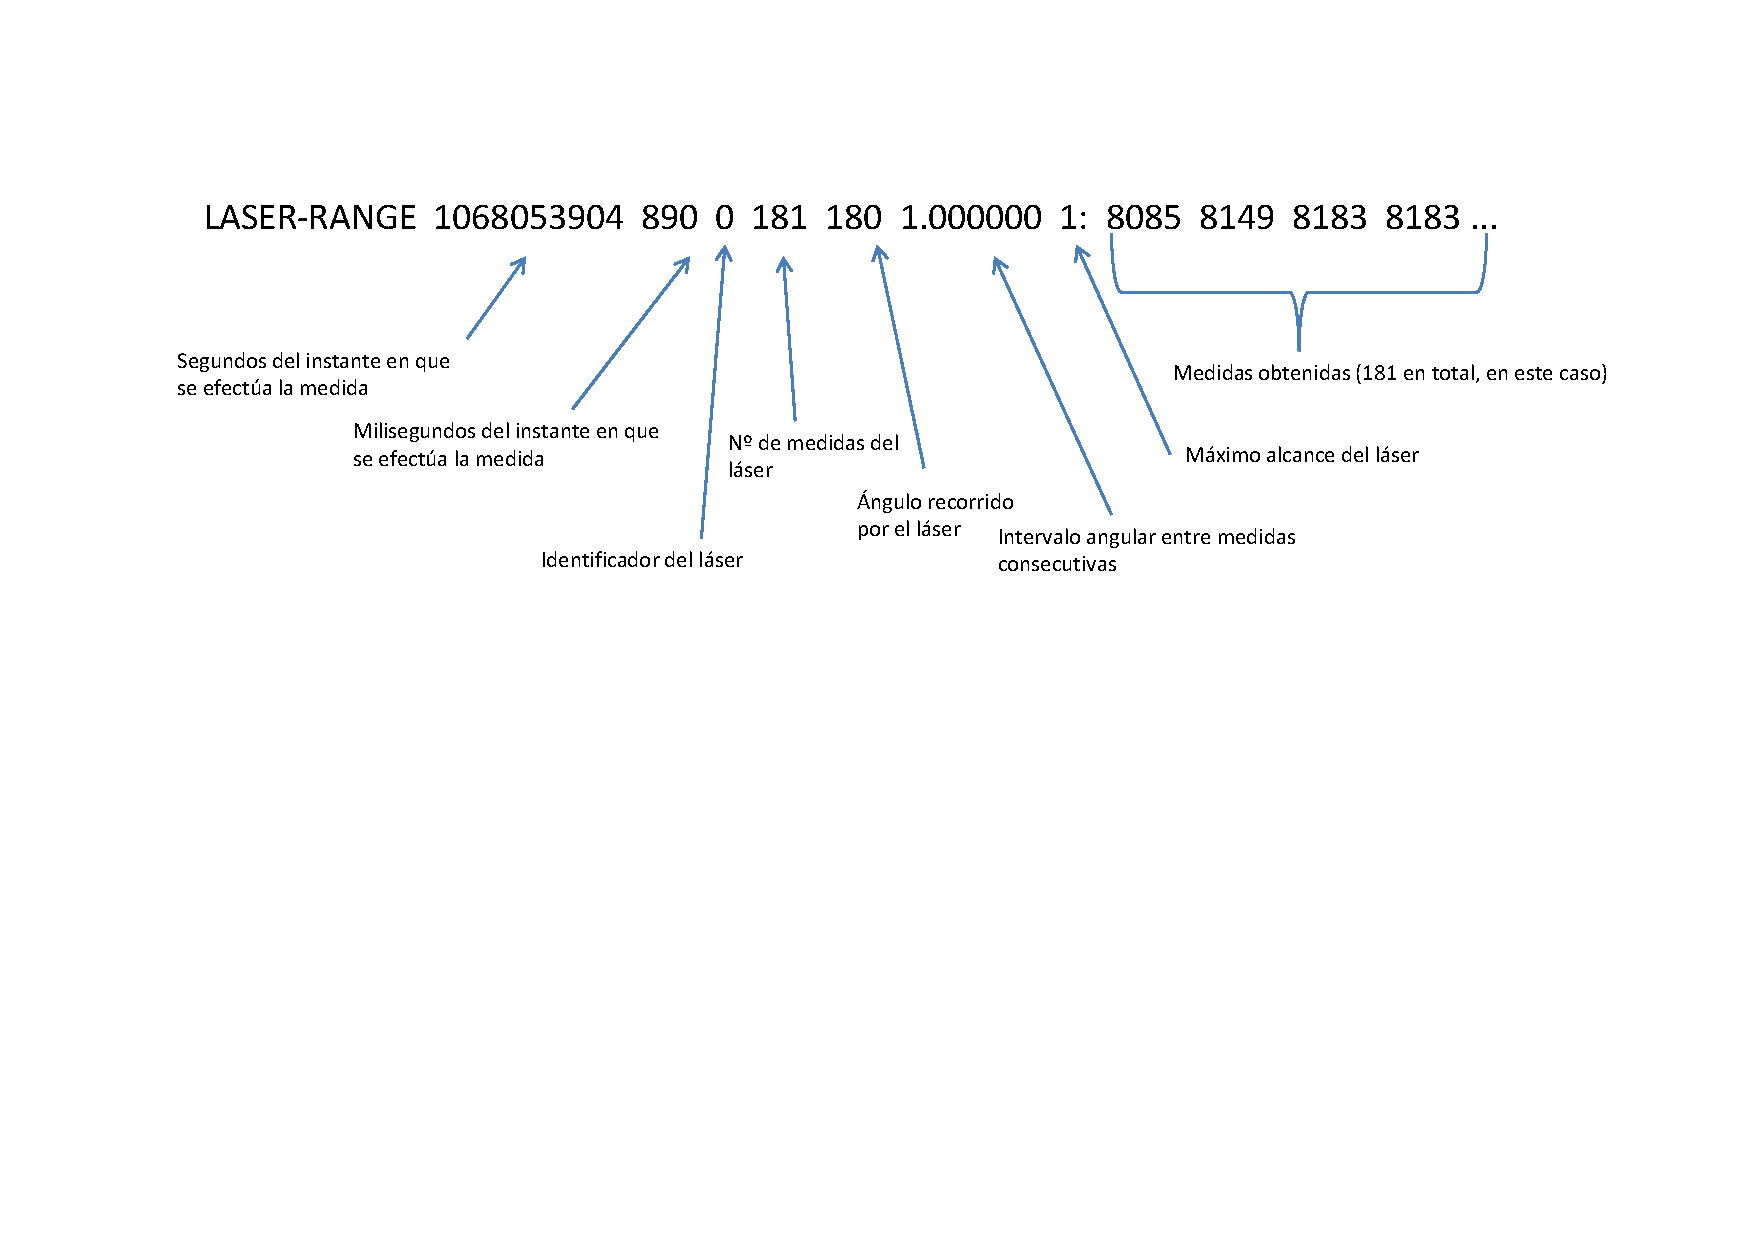
\includegraphics[width=0.9\textwidth]{laserfichero}\\
  \caption{Línea de fichero correspondiente a datos del láser}\label{fg:ficherolaser}
\end{figure}

\noindent
Si hay algún fallo en la lectura de los parámetros o de las medidas se devuelve $-1$. Si el fichero tiene el formato adecuado y se lee sin ningún problema se devuelve $0$.

\subsubsection{Save}

\prog{void Save(FILE* log\_file)}

\noindent
Esta función se emplea para escribir en un fichero los datos correspondientes a las medidas del láser.

\begin{itemize}
  \item \prog{log\_file}: fichero en el que se escribe la información del láser
\end{itemize}

\noindent
Se escribe el término LASER\_RANGE seguido del contenido de las variables \prog{time_stamp_seconds}, \prog{time_stamp_useconds}, \prog{id_laser}, \prog{num_med}, \prog{scan_angle}, \prog{scan\_resolution)} y \prog{max\_range} y dos puntos (':'). Después se escriben los valores de las diferentes medidas almacenadas en el vector \prog{med}. Todos los datos van separados por un espacio en blanco. En resumen, una llamada a esta función escribe una línea de fichero con el formato mostrado en \ref{fg:ficherolaser}.

\subsubsection {Serialize}
\prog{int Serialize(char* cad,int\& l,int size) const}
\subsubsection {DeSerialize}
\prog{int DeSerialize(char* cad,int\& l,int size)}

\vspace{0.2cm}
\noindent
Estas dos funciones no se han utilizado directamente, por lo que no se entra en detalles sobre su funcionamiento.

\subsection{La clase \prog{CProcLaserData}}
Se trata de una clase para el procesamiento y manejo de la información del láser. Sus métodos más utilizados son:

\subsubsection {SetOffset}

\prog{void SetOffset(float offx, float offy, float offz)}

\noindent
Esta función se emplea para establecer el offset del láser, es decir, indica la posición del mismo respecto al sistema de referencia local del robot.

\begin{itemize}
  \item \prog{offx}: desplazamiento del láser sobre la coordenada x del sistema de referencia local del robot
  \item \prog{offy}: desplazamiento del láser sobre la coordenada y del sistema de referencia local del robot
  \item \prog{offz}: desplazamiento del láser sobre la coordenada z del sistema de referencia local del robot
\end{itemize}

\noindent
En el robot Urbano el offset del láser viene dado por (0.168, 0.0, 1.2) y en el Pioneer P3AT los valores son (0.0, 0.0, 0.4).

Estos parámetros se pasan a las variables miembro \prog{off\_x}, \prog{off\_y} y \prog{off\_z}. Además, en ella se calculan las razones trigonométricas seno y coseno de los ángulos correspondientes a todas las diferentes medidas que pueden tomarse (intervalos de $0,5º$) y se guardan en sendos vectores \prog{cos\_alfa} y \prog{sen\_alfa}, de tamaño igual al máximo número de medidas posibles.

\subsubsection {DefineData}

\prog{int DefineData(const CRawLaserData\& d)}

\noindent
Permite calcular las coordenadas de los puntos correspondientes a las medidas del láser.

\begin{itemize}
  \item \prog{d}: objeto de la clase \prog{CRawLaserData} cuyos datos se van a procesar
\end{itemize}

\noindent
A partir del alcance de las medidas realizadas se ajusta el valor de las distancias hasta los obstáculos sobre cada ángulo de medida (almacenadas en el vector \prog{med}) y el resultado se guarda en un vector de enteros de nombre \prog{fmed}.
\noindent
Con el offset del láser y dichas medidas de distancia se obtienen las coordenadas de cada punto $i$ detectado mediante trigonometría:

$\mbox{med\_x}[i] = \mbox{off\_x}+fmed[i]\mbox{cos\_alfa}[istep]$

$\mbox{med\_y}[i] = \mbox{off\_y}+fmed[i]\mbox{sen\_alfa}[istep]$

$\mbox{med\_z}[i] = \mbox{off\_z}$,

\noindent
donde el valor de la variable \prog{step} puede ser $1$ ó $2$, viniendo dado por el número de medidas. De este modo se toman los ángulos de $0,5º$ en $0,5º$ o de $1º$ en $1º$.
\noindent
Los puntos 2D que así se obtienen (la coordenada $z$ se mantiene constante) se almacenan en el vector de la STL \prog{v}, miembro de esta clase.

La función devuelve un $0$ si el número de medidas es distinto de $181$ o de $361$ (en cuyo caso no se realiza procesamiento de las medidas, ya que ha de haber algún error) y un $1$ cuando el número de medidas es el adecuado y, por lo tanto, se han efectuado todas las operaciones de la definición de datos.

%subsection {AsignaParamLineSplit}
%
%prog{void AsignaParamLineSplit(float max_dis,float min_leng,int min_poin,float max_alcan,float max_sep)}
%
%signación de una serie de parámetros empleados para el cálculo de un polígono de puntos mediante el procedimiento que se indica en \ref{poligono}.
%
%begin{itemize}
% \item \prog{max_dis}:
% \item \prog{min_leng}:
% \item \prog{min_poin}:
% \item \prog{max_alcan}:
% \item \prog{max_sep}:
%end{itemize}
%
%Los valores utilizados con el robot Urbano son:
%prog{max_dis} $= 0.025$
%prog{min_leng} $= 0.6$
%prog{min_point} $= 11$
%prog{max_alcan} $= 8.0$
%prog{max_sep} $= 0.2$

\subsection{La clase \prog{CPosData}} \label{CPosData}

Esta clase es similar a la clase prog{CRawLaserData} pero se encarga del tratamiento de la información referente a la odometría. Dispone de variables miembro públicas en las que almacenar la posición odométrica y las velocidades del robot (\prog{posx}, \prog{posy}, \prog{posth}, \prog{vel_drive}, \prog{vel_steer}). Sus métodos son:

\subsubsection{Load}

\noindent
\prog{int Load(FILE* source\_file)}

\noindent
Esta función se emplea para leer de un fichero los datos correspondientes a las medidas de odometría.

\begin{itemize}
  \item \prog{source_file}: fichero del que se lee la información de la odometría
\end{itemize}

\noindent
Los resultados obtenidos sobre el instante en que se efectúa la medida, la coordenadas $x, y$ y $z$ de la posición, la velocidad de avance y la velocidad de giro se almacenan en las variables correspondientes: \prog{pos_temp}, \prog{pos_time_ms}, \prog{posx}, \prog{posy}, \prog{posth}, \prog{vel_drive} y \prog{vel_steer}.

En el ejemplo de la figura \ref{fg:ficheropos} se muestra cómo ha de ser el formato de una línea del fichero:

\begin{figure}[h]
  % Requires \usepackage{graphicx}
  \centering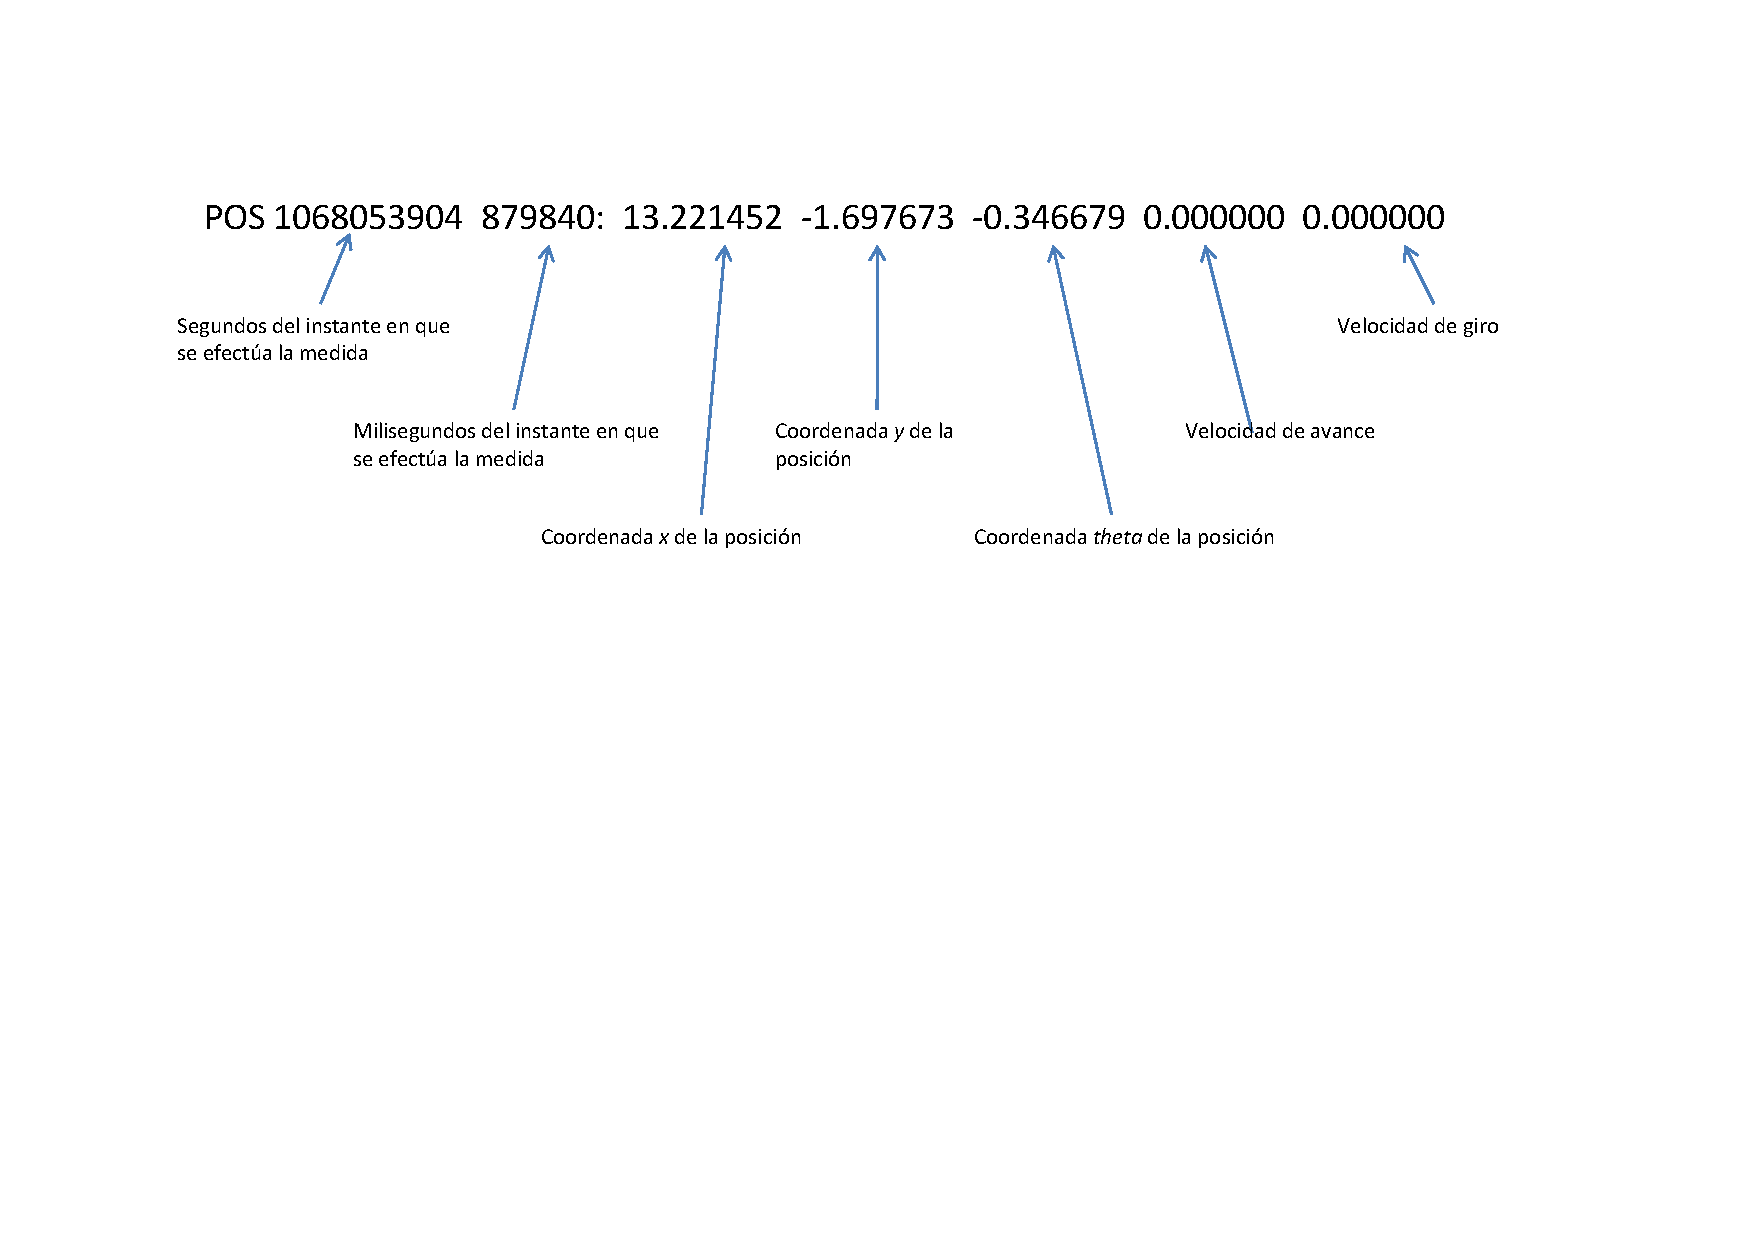
\includegraphics[width=0.9\textwidth]{posfichero}\\
  \caption{Línea de fichero correspondiente a datos de odometría}\label{fg:ficheropos}
\end{figure}

\noindent
Si hay algún fallo en la lectura de los parámetros o de las medidas se devuelve $-1$. Si el fichero tiene el formato adecuado y se lee sin ningún problema se devuelve $0$.

\subsubsection{Save}

\prog{void Save(FILE* log\_file)}

\noindent
Esta función se emplea para escribir en un fichero los datos correspondientes a las medidas de posición.

\begin{itemize}
  \item \prog{log\_file}: fichero en el que se escribe la información de la odometría
\end{itemize}

\noindent
Se escribe el término POS seguido del contenido de las variables \prog{pos_temp} y \prog{pos_time_ms} y dos puntos (':'). Después se escriben los valores de \prog{posx}, \prog{posy}, \prog{posth}, \prog{vel_drive} y \prog{vel_steer}. Todos los datos van separados por un espacio en blanco. En resumen, una llamada a esta función escribe una línea de fichero con el formato mostrado en \ref{fg:ficheropos}.

\subsubsection {Serialize}
\prog{int Serialize(char* cad,int\& l,int size) const}
\subsubsection {DeSerialize}
\prog{int DeSerialize(char* cad,int\& l,int size)}

\vspace{0.2cm}
\noindent
Al igual que en la clase \prog{CRawLaserData}, estas dos funciones no se han utilizado directamente, por lo que no se entra en detalles sobre su funcionamiento.

\subsection{La clase \prog{CRobotData}}
Esta clase se emplea para definir en cuál de los tres modos posibles se ha de conectar el robot y para procesar la información que permite su funcionamiento en los modos \emph{simulación} y \emph{fichero}. En ella se definen una serie de macros para indicar tipos de conexión (\prog{SIMU_CONN}, \prog{FILE_CONN}, \prog{REAL_CONN}) , tipos de datos (\prog{DATA_CONN_ERROR}, \prog{DATA_NONE}, \prog{DATA_ODOM}, \prog{DATA_LASER}, \prog{DATA_ODOM_LASER}, \prog{DATA_ODOM_INIT}) y tipos de estado (\prog{STATUS_NOT_INIT}, \prog{STATUS_CONNECTION_ERROR}, \prog{STATUS_CONNECTED}. Dentro de la clase se tienen dos variables miembro para el manejo de los datos de la odometría y del láser: \prog{odom_data}, de la clase \prog{CPosData}, y \prog{laser_data}, de la clase \prog{CRawLaserData}. Las principales funciones que se utilizan son las siguientes:

\subsubsection{Init}

\noindent
\prog{bool Init(int typ,const char* source)}

\noindent
Esta función se define como \prog{virtual} (para que pueda reescribirse en clases que hereden de ésta) y se emplea para establecer el modo de funcionamiento del robot. En caso de que el modo sea tipo fichero también se abre el fichero del que han de leerse los datos.

\begin{itemize}
  \item \prog{typ}: modo de funcionamiento del robot
  \item \prog{source}: nombre del fichero de datos o IP del robot real al que ha de conectarse el sistema
\end{itemize}

\noindent
En primer lugar se copia el parámetro \prog{source} en la cadena \prog{source_name}, variable miembro de la clase. Si la conexión es de tipo fichero, se abre el fichero de nombre \prog{source_name} en modo lectura. Si el fichero no existe la función devuelve \prog{false}. En caso contrario se guarda el modo de funcionamiento en la variable entera \prog{type}, también miembro de la clase, con los posibles valores \prog{FILE_CONN} (1), \prog{SIMU_CONN} (2) o \prog{SIMU_REAL} (3) y la función devuelve \prog{true}.

\subsubsection{SpeedValues}

\noindent
\prog{void SpeedValues(float vel_drive, float vel_steer)}

\noindent
Esta función se emplea para ajustar las velocidades al formato y rango adecuados.

\begin{itemize}
  \item \prog{vel_drive}: velocidad de avance que se le quiere dar al robot
  \item \prog{vel_steer}: velocidad de giro que se le quiere dar al robot
\end{itemize}

\noindent
Si la velocidad de avance es superior a 100 se le da valor 100 y si es menor que 0 se le da valor 0. Con la velocidad de giro se hace lo mismo en el intervalo [-100,100]. Ambos resultados se convierten a tipo \prog{char} y se almacenan en las variables de clase \prog{com_drive} y \prog{com_steer}.


\subsubsection{LoadData()}

\noindent
\prog{int LoadData()}

\noindent
Esta función se emplea para leer de un fichero los datos correspondientes a las medidas de odometría o del láser.

\noindent
En líneas generales, se lee la primera palabra de la línea del fichero abierto en la llamada a \prog{Init} en la que estemos y se mira si es igual a las cadenas "POS" o "LASER-RANGE". En el primer caso, se llama a la función \prog{Load} sobre el objeto \prog{pos_data} y en el segundo, a la función \prog{Load} del objeto \prog{laser_data}.

\noindent
Se devuelve el tipo de datos obtenido (\prog{DATA_CONN_ERROR}, \prog{DATA_ODOM}, \prog{DATA_LA}\prog{SER}\ldots).

\subsubsection{Simulate}

\noindent
\prog{int Simulate()}

\noindent
Esta función se emplea para actualizar la información de la odometría y del láser en el modo simulación.

\noindent
Respecto a la odometría, su actualización se realiza mediante composición de la posición odométrica anterior (accesible mediante \prog{odom_data}) con un vector de incrementos definido a partir de las velocidades \prog{com_drive} y \prog{com_steer}. Esta nueva posición obtenida se emplea para actualizar las variables \prog{posx}, \prog{posy} y \prog{posth} de \prog{odom_data}, de forma que queda disponible para la siguiente llamada. En lo relativo al láser, en la simulación se establece que el número de medidas es 181, que el ángulo que se cubre es de 180º, que las medidas se toman cada 1º y que el valor de todas ellas es \prog{laser_data.med[i]} $= 8000$.

\noindent
El valor que se devuelve es siempre \prog{DATA_ODOM_LASER}.

\subsubsection{UpdateData}

\noindent
\prog{int UpdateData()}

\noindent
Esta función es de tipo \prog{virtual} y se emplea para actualizar los datos de la odometría y del láser en los modos simulación y fichero.

\noindent
Si el tipo de conexión es \prog{FILE_CONN} se efectúa una llamada a la función \prog{LoadData}. Si el tipo de conexión es \prog{SIMU_CONN} se llama a la función \prog{Simulate}. En estos casos se devuelve el resultado de estas llamadas. Por defecto se devolverá \prog{DATA_CONN_ERROR} (tras realizarse la actualización del estado a \prog{STATUS_CONNECTION_ERROR}).

\vspace{0.2cm}
Otras funciones de la clase que se utilizan para guardar en un fichero los datos de la odometría y del láser son \prog{StartLogData} (crea y abre el fichero en el que escribir los datos), \prog{Log} (que a su vez llama a las funciones \prog{Save} de las variables \prog{odom_data} o \prog{laser_data} según corresponda) y \prog{StopLogData}.

\subsection{La clase CSocketNode}
Es la clase encargada de establecer las comunicaciones con el robot real mediante el uso de sockets. No se ha utilizado directamente.

\subsection{La clase CRobotDataReal}
Como se puede ver en el diagrama \ref{fg:uml}, esta clase hereda de \prog{CRobotData}y \prog{CSocketNode}. Es la clase necesaria para el funcionamiento del robot en modo real. Sus métodos más importantes son los siguientes:

\subsubsection{Init}

\noindent
\prog{bool Init(int typ,const char* source)}

\noindent
Esta función se emplea para establecer el modo de funcionamiento del robot y efectuar la conexión en el caso de modo real.
\begin{itemize}
  \item \prog{typ}: modo de funcionamiento del robot
  \item \prog{source}: nombre del fichero de datos o IP del robot real al que ha de conectarse el sistema
\end{itemize}

\noindent
En ella se hace una llamada a la función \prog{Init} de la clase \prog{CRobotData}, de forma que sólo es necesario añadir la funcionalidad de establecer conexión en modo real. En ese caso, se leen del parámetro \prog{source} la dirección IP y el puerto de escucha del servidor con el que se ha de realizar la conexión. Una vez se tienen estos datos, se inicia un socket cliente y se lanza el thread que se encarga de la comunicación entre éste y el servidor. Para ello se utilizan funciones de \prog{CSocketNode}. El valor de retorno es siempre \prog{true}.

\subsubsection{TransferData}

\noindent
\prog{int TransferData()}

\noindent
Esta función se emplea para enviar los valores de velocidad al robot y recibir de él la información sobre la odometría y las medidas del láser.

\noindent
Los datos de velocidad se envían en el formato "TransferData 100 -10", donde 100 sería la velocidad de avance y -10, la velocidad de giro. Los datos de odometría y del láser que se reciben se pasan a las variables \prog{odom_data} y \prog{laser_data} por medio de sus métodos \prog{DeSerialize}, de modo que quedan procesados para su utilización en el resto del programa.


\subsubsection{UpdateData}

\noindent
\prog{int UpdateData()}

\noindent
Esta función se emplea para actualizar los datos de la odometría y del láser en el modo real.

\noindent
Si el tipo de conexión es \prog{REAL_CONN} se efectúa una llamada a la función \prog{TransferData} y posteriormente a \prog{Log} para guardar los datos obtenidos en un fichero (siempre que previamente se haya empleado \prog{StartLogData}). En caso contrario (\prog{SIMU_CONN} o \prog{FILE_CONN}) se llama a la función \prog{Update} de la clase \prog{CRobotData}.

\noindent
Se devuelve el tipo de datos obtenido (\prog{DATA_CONN_ERROR}, \prog{DATA_ODOM}, \prog{DATA_LASER}, \prog{DATA_ODOM_LASER} o \prog{DATA_NONE}).




% -*- coding: utf-8 -*-

\chapter{Localización y mapas}

El sistema de localización realizado no incorpora la construcción simultánea de mapas de los tipos descritos en el capítulo de Estado del Arte sino que elabora y luego va actualizando un mapa de puntos a partir de las observaciones correspondientes a las medidas del láser. Son los puntos que ya forman parte del mapa los que se utilizan para la localización en cada instante. Se trata de un método de \emph{máxima probabilidad incremental} basado en el filtro extendido de Kalman.

\section{Aplicación del EKF a la localización del robot: descripción del algoritmo}

En el problema que se trata, el estado queda definido por la posición del robot, $[x_{R},y_{R},\theta_{R}]^{T}$. Las medidas de la odometría (incrementales, luego referenciadas al sistema de coordenadas local del robot) constituyen las entradas al sistema, $\vec{u}=\pmatrix{u_{x}\cr u_{y}\cr \theta_{u}}$, en cada instante (se suprimen sus subíndices de tiempo para simplificar la notación; siempre se utilizan las últimas medidas disponibles). De esta forma, el modelo de estado identificable con  \ref{eq:estado_nolineal} es:

 \begin{equation}\label{estado_robot}
    \vec{x}_{R_{k}} = \vec{x}_{R_{k-1}}\oplus \vec{u} +\vec{\rho}_{\rho},
 \end{equation}

\noindent
siendo $\oplus$ el operador composición de transformaciones relativas.

\paragraph{Etapa de predicción.}
De acuerdo con esto, la predicción del estado dada por \ref{eq:x_predictionEKF} será:
\begin{equation}\label{eq:x_prediction_robot}
     \pmatrix{\tilde{x}_{R_{k}}\cr \tilde{y}_{R_{k}}\cr \tilde{\theta}_{R_{k}}} =
     \pmatrix{\hat{x}_{R_{k-1}}+u_{x}cos\hat{\theta}_{R_{k-1}}-u_{y}sen\hat{\theta}_{R_{k-1}}\cr \hat{y}_{R_{k-1}}+u_{x}sen\hat{\theta}_{R_{k-1}}+u_{y}cos\hat{\theta}_{R_{k-1}} \cr \hat{\theta}_{R_{k-1}}+\theta_{u}}
\end{equation}

Para la matriz de covarianza de $x_{k}$ la ecuación \ref{eq:P_predictionEKF} varía ligeramente ya que lo que se conoce no es la matriz de covarianza del proceso conjunto, $Q_{p}$,sino la covarianza del ruido presente en la odometría $\vec{u}$. Si esta variable gaussiana se representa por $\vec{u}_{k}\sim N(\hat{\vec{u}}_{k},Q)$ (tomaremos un valor constante para la covarianza del ruido en el incremento de odometría medido a partir de los datos de los encoders) la predicción de la covarianza del estado será:

\begin{equation}\label{eq:P_prediction_robot}
    \tilde{P}_{k} = F_{x}\hat{P}_{k-1}F_{x}^{T}+F_{u}QF_{u}^{T},
\end{equation}

\noindent
donde $F_{x} = \frac{\delta f}{\delta x}\mid _{\tilde{x}_k}$ y $F_{u} = \frac{\delta f}{\delta u}\mid _{\tilde{x}_k}$ (se emplea la mejor estimación del estado disponible hasta el momento).

El resultado del cálculo de estas matrices jacobianas se incluye en el Anexo~\ref{ap:transformaciones}.

El algoritmo se inicia partiendo de $\hat{x}_{0} = 0, \hat{P}_{0} = 0$.

\paragraph{Etapa de corrección.}
Las medidas, observaciones realizadas por el láser, se relacionan con el estado de forma implícita mediante composición con él y comparación con los puntos del mapa que se utilice. Como puede verse en la figura \ref{fg:medidas}, la expresión que liga idealmente el estado con la observación i por medio del punto del mapa j asociado a ella será:

\begin{equation}\label{eq:medidas}
    \vec{h_{ij}} = \vec{x_{R}} \oplus \vec{o_{i}} - \vec{l_{j}} = \vec{0},
\end{equation}

Aplicando la definición del operador $\oplus$ (Anexo \ref{ap:transformaciones}), la ecuación \ref{eq:medidas} queda:

\begin{equation}\label{eq:hij}
    \vec{h_{ij}} = \pmatrix{-x_{lj}+x_{R}+o_{ix}cos\theta_{R}-o_{iy}sen\theta_{R}\cr -y_{lj}+y_{R}+o_{ix}sen\theta_{R}+o_{iy}cos\theta_{R}} = \vec{0},
\end{equation}

\noindent
como puede obtenerse a partir de la figura \ref{fg:medidas}.

\begin{figure}[h]
  % Requires \usepackage{graphicx}
  \centering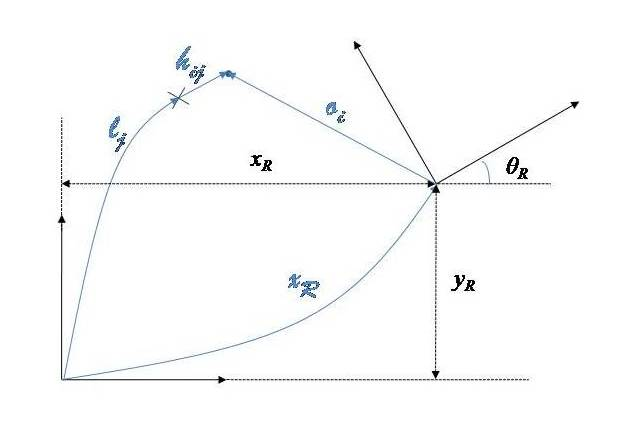
\includegraphics[scale=0.7]{dibujo1}\\
  \caption{Representación de la ecuación de medida del robot}\label{fg:medidas}
\end{figure}


Denotando $H_{x_{ij_{k}}} = \frac{\delta \vec{h_{ij}}}{\delta \vec{x}}\mid _{\tilde{x}_k,z_{k}}$ y $H_{z_{ij_{k}}} = \frac{\delta \vec{h_{ij}}}{\delta \vec{z}}\mid _{\tilde{x}_k,z_{k}}$ para cada iteración k, la matriz de covarianza de una innovación individual viene dada por \ref{eq:SEKF_im}:

\begin{equation}\label{eq:Sij_robot}
    S_{ij_{k}} = H_{x_{ij_{k}}}\tilde{P}_{k}H_{x_{ij_{k}}}^{T}+H_{z_{ij_{k}}}RH_{z_{ij_{k}}}^{T}
\end{equation}

Como puede verse en la ecuación \ref{eq:Sij_robot}, la covarianza en las medidas del láser también se tomará como constante.

El cálculo de la distancia de Mahalanobis de la innovación $h_{ij_{k}}$ mediante esta matriz $S_{k}$ permitirá realizar la asociación de cada observación \emph{i} al punto del mapa \emph{j} para el cual esa distancia sea mínima. Si dicha asociación supera el test de Mahalanobis, se tendrá en cuenta para corregir la posición del robot, en caso contrario se podrá añadir la observación como nuevo punto del mapa.De entre todas las matrices $h_{ij}, H_{x_{ij}} y H_{z{ij}}$ calculadas para cada observación asociada a un punto del mapa se utilizarán únicamente las correspondientes a dicho punto. Estas matrices se denotarán $hi_{min}, Hxi_{min}, Hzi_{min}$.

Según se van asociando observaciones, se tienen más medidas que utilizar. Por ello, las dimensiones de las matrices $h, H_{x}, H_{z} y R$ irán creciendo al irse añadiendo datos. Su tamaño final en cada iteración determinará las dimensiones de S y K.

Para un número t de observaciones asociadas en la iteración k, se tiene:

\[ \mbox{dim}  h_{k}            =   2t \times 1 \]
\[ \mbox{dim}  H_{x_{k}}     =  2t \times 3 \]
\[ \mbox{dim}  H_{z_{k}}     =  2t \times 2t \]
\[ \mbox{dim}  R_{k}            =  2t \times 2t \]

Con lo que la matriz S global calculada a partir de ellas por medio de la ecuación~\ref{eq:SEKF_im} será:
\begin{equation}\label{eq:S_robot}
    S_{k} = H_{x_{k}}\tilde{P}_{k}H_{x_{k}}^{T}+H_{z_{k}}RH_{z_{k}}^{T}
\end{equation}
y tendrá dimensión ($2t \times 2t$).

La matriz de Kalman del sistema, viene dada por \ref{eq:KEKF_im}:
\begin{equation}\label{eq:K_robot}
    K_{k} = \tilde{P}_{k}H_{x_{k}}^{T}S_{k}^{-1}
\end{equation}
por lo que su tamaño será ($3 \times 2t$).

Finalmente, los valores corregidos de la posición del robot y su covarianza se obtienen a partir de la predicción de acuerdo con \ref{eq:x_estimationIm} y \ref{eq:P_estimationEKF_im}:
\begin{equation}\label{eq:x_robot}
    \hat{x}_{k} = \tilde{x}_{k} - K_{k}h_{k}
\end{equation}
\begin{equation}\label{eq:P_robot}
    \hat{P}_{k} = (I-K_{k}H_{x_{k}})\tilde{P}_{k}
\end{equation}


\section{Consideraciones sobre el coste \\ computacional de la localización} \label{computacional}

El coste computacional de la etapa de corrección del algoritmo puede llevar a tiempos de procesamiento altos, lo que conduce a un comportamiento del sistema poco eficaz. A continuación se realiza un análisis del mismo y se identifican las principales fuentes de retardo en el cómputo de la posición corregida.

Para $n$ puntos en el mapa y $t$ observaciones adquiridas por el láser, el coste computacional de la etapa de asociación de datos es de orden $O(nt)$.

El cálculo de la matriz de ganancia de Kalman se realiza mediante \ref{eq:K_robot}. Al tener la matriz $\tilde{P}_{k}H_{x_{k}}^{T}$ dimensión ($3 \times 2t$) y $S$ dimensión ($2t \times 2t$), el coste computacional para hallar la matriz $K$ será $O(t^{3})$.

Sin variar el coste computacional, puede verse que una forma sencilla de reducir el tiempo de cálculo consiste en reducir el número de observaciones a tener en cuenta. Las observaciones que se encuentran muy alejadas del robot (distancias superiores a 6m) directamente son ignoradas. El láser proporciona medidas a intervalos de 1º (181 medidas en total) o bien a intervalos de 0.5º (361 medidas en total). Utilizando sólo una de cada dos observaciones asociadas se logra una reducción de tiempo considerable sin que se aprecien pérdidas en los resultados de la localización.

Las operaciones que inicialmente consumían más tiempo en el procesamiento de las observaciones eran la declaración de las matrices $h_{ij}, H_{x_{ij}} y H_{z{ij}}$ para todas las innovaciones y el ir ampliando las matrices $h, H_{x}, H_{z}$ y $R$ por filas o por columnas a medida que se asociaban más datos, con la consiguiente reserva de memoria cada vez.

En relación al primer punto, se optó por realizar una única declaración al principio de cada proceso de corrección e inicializar las componentes de las matrices que permanecen constantes para todas las observaciones.

Respecto al segundo punto, también se hace una reserva inicial de memoria para el tamaño máximo de las matrices $h$ y $H_{x}$ y según se van asociando observaciones se van incluyendo componentes en ellas. Las matrices $H_{z}$ de las sucesivas asociaciones se van guardando en un vector de la STL.

La última mejora introducida se centra en la obtención de la matriz $S$ (definida al comienzo de la etapa de corrección sin especificación de tamaño) y se basa en el hecho de que $H_{z}$ y $R$ son matrices diagonales por bloques, por lo que tienen muchas componentes nulas. El primer término de $S$ se calcula a partir de la matriz $PHt = \tilde{P}_{k}H_{x_{k}}^{T}$, que puede ser posteriormente utilizada en el cálculo de $K$. A continuación se va sumando a cada bloque ($2 \times 2$) de la diagonal principal el producto $H_{z}RH_{z}^{T}$ de cada observación, efectuándose así la operación únicamente sobre las componentes que sufren alguna modificación.

\section{Algoritmo de borrado de puntos \\dinámicos del mapa} \label{poligono}
Para eliminar los puntos que se añadieron al mapa en un momento dado pero dejan de corresponder a asociaciones con las medidas del láser (dejan de observarse), se construye un polígono a partir de estas medidas de modo que los puntos que quedan dentro del mismo pueden ser borrados.

La obtención del polígono se hace de forma recursiva, empleándose en líneas generales el siguiente procedimiento:
\begin{itemize}
  \item Se toma el segmento que une la primera observación con la última.
  \item Se mira cuál es la observación intermedia que está más separada del segmento.
  \item Si esta separación es suficiente, se repite el proceso entre la primera observación y la más separada y entre ésta y la última.
  \item Cuando un segmento no tiene ninguna observación a más distancia que el umbral establecido, se añaden sus extremos como vértices del polígono.
\end{itemize}

Cuando alguna observación está fuera del alcance de medida, la subdivisión se realiza entre la primera observación y la anterior a aquélla y entre la observación siguiente a la medida lejana y la última observación tomada. En el caso de que una observación esté muy separada de la anterior, se realiza el procedimiento de subdivisión para el bloque de puntos previo a la separación y después para el bloque de puntos siguientes a esa separación.

A partir del polígono determinado en cada instante, se eliminan aquellos puntos de su interior que no están muy próximos a la frontera. Dada la forma en que se construye el polígono, esta última condición es necesaria como medida de precaución para no borrar puntos del mapa indebidamente.

\begin{figure}[h]
  % Requires \usepackage{graphicx}
  \centering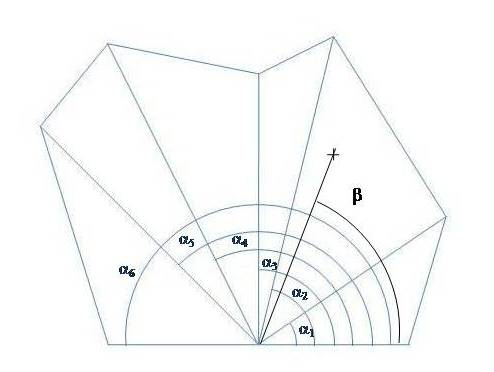
\includegraphics[scale=0.7]{poligono}\\
  \caption{ Ángulos a medir para ver si un punto está dentro de un polígono no convexo}\label{fg:poligono}
\end{figure}


El polígono será, por lo general, no convexo. El algoritmo utilizado para ver si un punto se encuentra en su interior requiere medir los ángulos $\alpha_{1},\alpha_{2},...\alpha_{v}$ indicados en la figura \ref{fg:poligono}. Para cada punto del mapa (tras calcular sus coordenadas en el sistema de referencia local en el láser), se halla el valor del ángulo $\beta$ y se mira entre qué dos alphas está comprendido ($\alpha_{1}$ y $\alpha_{2}$ en el caso de la figura). Con esto se seleccionan dos vértices que servirán para ver si el punto del mapa está dentro del polígono. Se mide la distancia del robot al punto del mapa y se compara con la distancia entre el robot y el vértice de los dos anteriores que sea más cercano al mismo(criterio conservador). Si resulta ser menor, será que el punto se encuentra dentro del polígono.

De este modo, para cada punto del mapa sólo ha de calcularse un ángulo. Esto permite una velocidad de ejecución aceptable.

\section{La clase \prog{CKalman\_ Loc}}
Esta clase se ha creado para gestionar las operaciones relacionadas con el tratamiento de los mapas de puntos que se utilizan y, fundamentalmente, la localización del robot en cada instante. Aparte del constructor, contiene las funciones que se describen brevemente a continuación.

\subsection{\prog{KalmanPos}}

%\prog{void KalmanPos(float inc_odom_x, float inc_ odom_ y, float inc_odom_theta}

\begin{lstlisting}[basicstyle=\small\ttfamily,language=C]
void KalmanPos(float inc_odom_x, float inc_ odom_ y,
         float inc_odom_theta)
\end{lstlisting}

\noindent
En esta función se realizan los cálculos correspondientes a la fase de predicción del algoritmo de localización.

\begin{itemize}
  \item \prog{inc_odom_x}: incremento de odometría medido sobre el eje x del sistema local en el robot
  \item \prog{inc_odom_y}: incremento de odometría medido sobre el eje y del sistema local en el robot
  \item \prog{inc_odom_theta}: variación incremental odométrica en la orientación del robot
\end{itemize}

La posición resultante se almacena en una variable miembro de tipo \prog{Matrix} llamada \prog{pos_robot_kalman}.

\subsection{\prog{KalmanUpdate}}

\prog{void KalmanUpdate(const std::vector<Point2D>\& v)}

\noindent
Esta función efectúa la fase de corrección de la localización a partir de la posición obtenida mediante la predicción y de las observaciones que se le pasan.

\begin{itemize}
  \item \prog{v}: vector de la STL que contiene los puntos correspondientes a las observaciones realizadas por el láser
\end{itemize}

El resultado se guarda nuevamente en la variable \prog{pos\_robot\_kalman}.

Inicialmente el mapa (vector de la STL que almacena objetos de la clase Point2D) se encontrará vacío si no se utiliza uno ya realizado. Como ya se ha explicado, las observaciones que no se asocian a ningún punto del mapa se añaden como puntos del mismo si así se selecciona mediante la variable miembro \prog{actualiza} (controlable desde el cuadro de diálogo mediante un \emph{Check box})

%Para los puntos del mapa que no se asocian a una observación, pero se encuentran cercanos a ella o a la mejor estimación de la posición del robot en ese momento,
Para cada uno de los puntos del mapa se comprueba si están en el interior del polígono de observaciones mediante la función \prog{PuntoEnPol} (\ref{PuntoEnPol}). En caso afirmativo, y si así lo indica la variable miembro \prog{borrar}, se eliminan del vector \prog{mapa}. Esto es posible porque el polígono es previamente calculado en cada iteración mediante un objeto de la clase \prog{CProcLaserData} perteneciente a la clase \prog{CRobot}. Sus puntos se almacenan en un vector de la STL al cual apunta un puntero miembro de \prog{CKalmanLoc}, \prog{pol}.

\subsection{\prog{GuardarMapa}}\label{GuardarMapa}

\prog{void GuardarMapa(LPTSTR path)}

\noindent
Esta función sirve para guardar un fichero de puntos del mapa de forma que si se dispone de un buen mapa no sea necesario realizar uno nuevo. También resulta útil para examinar los mapas generados o para agilizar algunas pruebas.

\begin{itemize}
  \item path:  \emph{path} en el que guardar un fichero de texto que contendrá dos columnas con las coordenadas de los puntos de un mapa
\end{itemize}

\subsection{\prog{LeerMapa}}

\prog{void LeerMapa(LPTSTR path)}

\noindent
Esta función se emplea para descargar un mapa ya creado (por medio de \prog{GuardarMapa}, \ref{GuardarMapa}, generalmente).

\begin{itemize}
  \item \prog{path}:  \emph{path} de un fichero de texto ya existente en el que se definen los puntos de un mapa mediante dos columnas de coordenadas
\end{itemize}

A medida que se van leyendo puntos se guardan en el vector \prog{mapa}.

\paragraph{Nota.}
Para que las dos funciones anteriores se ejecuten adecuadamente en Visual Studio .NET 2005 en los \emph{Settings} o \emph{Propiedades} del proyecto no debe marcarse la utilización del juego de caracteres Unicode.

\subsection{\prog{PuntoEnPol}}\label{PuntoEnPol}

\prog{int PuntoEnPol(int k)}

\noindent
Esta función sirve para determinar si un punto del mapa se encuentra en el interior del polígono al que apunta el puntero \prog{pol}.

\begin{itemize}
  \item \prog{k}: índice del punto del mapa cuya pertenencia al polígono se quiere determinar
\end{itemize}

Si el punto $k$ del vector \prog{mapa} está en el interior del polígono de observaciones de acuerdo con los criterios establecidos, se devuelve un 1 para que sea eliminado del mapa. En caso contrario la función devuelve un 0.


\section { Otras funciones de la clase \prog{CProcLaserData}}

\subsection {\prog{CalculaPol}}

\prog{void CalculaPol()}

\noindent
Esta función se utiliza para crear un polígono envolvente de las observaciones realizadas por el láser.
Inicializa el número de puntos que lo forman a 0 y después hace una llamada a la función recursiva \prog{Split}, que se describe a continuación.

\subsection {\prog{Split}}

\prog{void Split(int primer, int segun)}

\noindent
Función recursiva que permite ir obteniendo los segmentos que formarán el polígono con las propiedades mencionadas.

\begin{itemize}
  \item \prog{primer}: índice de la observación a partir de la cual se van a hallar nuevos segmentos
  \item \prog{segun}: índice de la observación hasta la cual se calculan segmentos
\end{itemize}

Se trata de la implementación del proceso descrito al principio de \ref{poligono}.

\paragraph{Nota.}
Las dos últimas funciones no han sido realizadas dentro del proyecto. Se incluyen en este capítulo en lugar de en el anterior para que pueda comprenderse mejor su utilización.

\subsection{\prog{ConviertePol}}

\prog{void ConviertePol(Matrix pos)}

\noindent
Esta función calcula las coordenadas de los vértices del polígono en el sistema de referencia global.

\begin{itemize}
  \item \prog{pos}: posición del robot. Se emplea la mejor estimación disponible en cada iteración.
\end{itemize}

Se utiliza principalmente para trazar el dibujo del polígono y para medir distancias de los puntos del mapa a los lados del mismo.

\subsection{\prog{PolAng}}

\prog{void PolAng(Matrix pos)}

\noindent
Método que se emplea para calcular los ángulos $\alpha$ de la figura \ref{fg:poligono}.

\begin{itemize}
  \item \prog{pos}: posición del robot. Se emplea la mejor estimación disponible en cada iteración.
\end{itemize}

Se aplica un coeficiente de acercamiento de los vértices del polígono al robot y posteriormente se calcula el ángulo $\alpha$ de cada vértice. Estos ángulos se almacenan en un vector \prog{angulos} de la STL variable miembro de la clase.

\section{Pruebas y resultados}
Las pruebas relativas a la localización y a la construcción de mapas de puntos se han efectuado en los modos fichero y real. En simulación las medidas del láser se consideran con alcance constante, por lo que no aportan información que permita la localización.

\subsection{Pruebas en modo \emph{fichero}}
En estas pruebas, se han empleado datos de odometría y del láser obtenidos con diferentes robots y en diferentes entornos por Diego Rodríguez-Losada y otros investigadores que han trabajado con él. Se ha estudiado el funcionamiento del algoritmo implementado por medio de ficheros que contienen esa información sensorial sin procesar. En ellos se alternan líneas del tipo representado en la figura \ref{fg:ficheropos} (datos de la odometría) y líneas del tipo representado en la figura \ref{fg:ficherolaser} (datos de medidas del láser). Estas pruebas resultan de mucha utilidad ya que utilizan gran variedad de datos y permiten evaluar el funcionamiento del sistema en entornos muy distintos y con medidas de diferentes características.

\subsubsection{Utilización de datos tomados en el laboratorio de DISAM-UPM}
En este caso, los datos empleados contienen 181 medidas del láser cada vez. Debe recordarse que, por motivos de coste computacional, el algoritmo de localización emplea una de cada dos de ellas. Como estos datos fueron obtenidos con el robot Urbano, no es necesario modificar el \emph{offset} del láser utilizado en el programa.

\paragraph{Prueba 1.}
En esta prueba se han utilizado los siguientes parámetros:
\begin{itemize}
  \item desviación típica del ruido de la odometría introducida en el filtro de Kalman: $\sigma_{odom} = 0.1$
  \item desviación típica del ruido de las medidas del láser: $\sigma_{med} = 0.3$
  \item ruido adicional: $\sigma_{extra} = 0$
  \item borrado de puntos dinámicos del mapa: $borrar = false$
  \item incorporación de nuevos puntos al mapa: $actualiza = true$
\end{itemize}


\paragraph{Resultados:}

En la figura \ref{fg:labo1} se puede ver el resultado de la ejecución del programa con las condiciones indicadas. Las sucesivas posiciones del robot según los datos de odometría disponibles serían las representadas en color verde, mientras que la trayectoria corregida mediante el filtro de Kalman es la mostrada en color rojo. Los puntos del mapa creado aparecen en color negro.

\begin{figure}[h]
  % Requires \usepackage{graphicx}
  \centering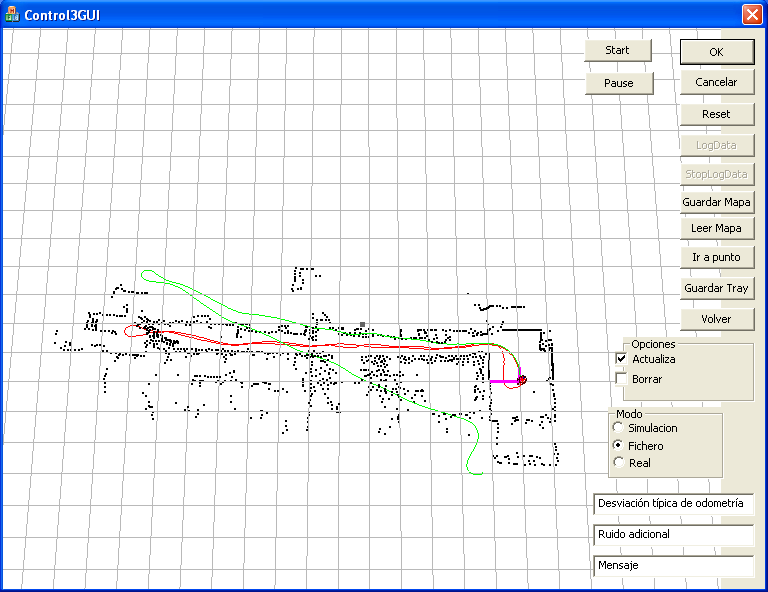
\includegraphics[scale=0.4]{labo1}\\
  \caption{Primer experimento con datos del laboratorio}\label{fg:labo1}
\end{figure}

Se puede apreciar el buen funcionamiento del algoritmo, que permite situar el robot adecuadamente en el mapa y ofrece un valor de posición final muy similar al de la posición de partida del robot.

El tiempo total empleado en la obtención del mapa y en el cálculo de la trayectoria corregida es: 3.54min.

\paragraph{Prueba 2.}
En esta prueba se han utilizado los siguientes parámetros:
\begin{itemize}
  \item desviación típica del ruido de la odometría introducida en el filtro de Kalman: $\sigma_{odom} = 0.3$
  \item desviación típica del ruido de las medidas del láser: $\sigma_{med} = 0.3$
  \item ruido adicional: $\sigma_{extra} = 0$
  \item borrado de puntos dinámicos del mapa: $borrar = false$
  \item incorporación de nuevos puntos al mapa: $actualiza = true$
\end{itemize}


\paragraph{Resultados:}

\begin{figure}[h]
  % Requires \usepackage{graphicx}
  \centering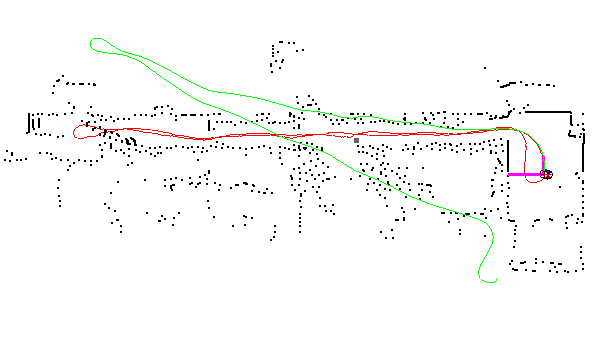
\includegraphics[scale=0.4]{labo2}\\
  \caption{Segundo experimento con datos del laboratorio}\label{fg:labo2}
\end{figure}

Al no ser excesivamente malos los datos de la odometría, no se logran demasiadas mejoras en la localización tras otorgar una mayor importancia a las medidas del láser frente a dichos datos. Sin embargo, puede verse que la parte izquierda del mapa obtenido en este caso es más precisa (figura \ref{fg:labo2}).

El tiempo total empleado en la obtención del mapa y en el cálculo de la trayectoria es: 3.22min. La disminución del tiempo de ejecución es resultado de la mejor asociación de observaciones a puntos del mapa, que hace que éste tenga un menor tamaño.

\paragraph{Prueba 3.}
En esta prueba se han utilizado los siguientes parámetros:
\begin{itemize}
  \item desviación típica del ruido de la odometría introducida en el filtro de Kalman: $\sigma_{odom} = 0.3$
  \item desviación típica del ruido de las medidas del láser: $\sigma_{med} = 0.3$
  \item ruido adicional: $\sigma_{extra} = 0$
  \item borrado de puntos dinámicos del mapa: $borrar = true$
  \item incorporación de nuevos puntos al mapa: $actualiza = true$
\end{itemize}


\paragraph{Resultados:}

\begin{figure}[h]
  % Requires \usepackage{graphicx}
  \centering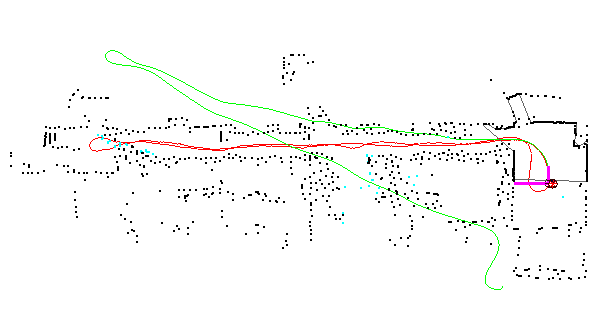
\includegraphics[scale=0.4]{labo3}\\
  \caption{Tercer experimento con datos del laboratorio}\label{fg:labo3}
\end{figure}

En la figura \ref{fg:labo3} puede verse que cuando se tomaron estos datos había algunas personas moviéndose cerca del recorrido realizado por el robot. Esta opción de ejecución permite borrar del mapa los puntos correspondientes a las posiciones que fueron ocupando (puntos de color cyan en la figura). La localización no resulta afectada de manera significativa por el borrado de dichos puntos. En la figura queda representado el polígono envolvente de las medidas del láser correspondiente a la última posición del robot.

El tiempo total empleado en la obtención del mapa y en el cálculo de la trayectoria corregida es: 3.63min. El cálculo de los puntos del polígono, el de los ángulos necesarios para aplicar el algoritmo de borrado y el análisis de los puntos del mapa no asociados a cada observación en las sucesivas iteraciones( llamadas al método \prog{KalmanUpdate}) provocan un cierto retardo en la ejecución del programa. Este tiempo, no obstante, es considerablemente inferior al correspondiente a otros algoritmos para examinar si un punto pertenece o no a un polígono (algoritmo de Jordan, algoritmo radial\ldots). Además, cada observación nueva ha de compararse con un número menor de puntos del mapa, con lo que en algunos casos el retardo puede quedar prácticamente compensado.

\paragraph{Prueba 4.} 
En esta prueba se han utilizado los siguientes parámetros:

\begin{itemize}
  \item desviación típica del ruido de la odometría introducida en el filtro de Kalman: $\sigma_{odom} = 0.6$
  \item desviación típica del ruido de las medidas del láser: $\sigma_{med} = 0.3$
  \item ruido adicional: $\sigma_{extra} = 0.005$
  \item borrado de puntos dinámicos del mapa: $borrar = false$
  \item incorporación de nuevos puntos al mapa: $actualiza = true$
\end{itemize}

\paragraph{Resultados:}

\begin{figure}[h]
  \centering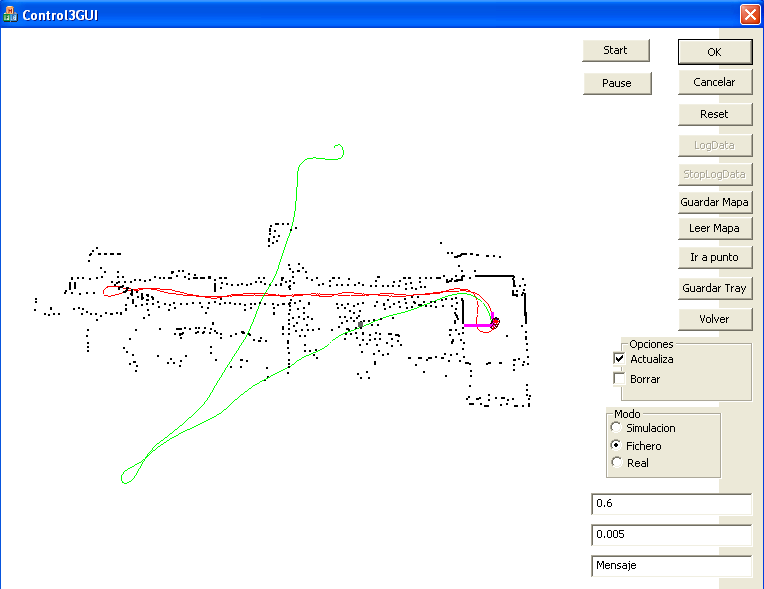
\includegraphics[scale=0.4]{labo4}\\
  \caption{Cuarto experimento con datos del laboratorio}\label{fg:labo4}
\end{figure}

Como puede verse en la figura \ref{fg:labo4}, al inyectarse algo de ruido añadido en las medidas odométricas, la posición del robot estimada en base a dichas medidas está muy alejada de la real. Sin embargo, mediante el algoritmo de localización se sigue obteniendo un buen resultado con sólo volver a incrementar el parámetro considerado en el EKF como varianza del ruido de la odometría.

El tiempo total empleado en la obtención del mapa y en el cálculo de la trayectoria corregida es: 3.15min. Tras tenerse en cuenta que la varianza del ruido de la odometría debe ser algo superior, se mejora la asociación de datos y con ello disminuye el tiempo de procesamiento.

\clearpage
\subsubsection{Utilización de datos de Intel}

Con estos datos, el número de medidas del láser disponibles en cada momento es 361. Esto repercute en el tiempo de procesamiento.

\paragraph{Prueba 1.}
En esta prueba se han utilizado los siguientes parámetros:
\begin{itemize}
  \item desviación típica del ruido de la odometría introducida en el filtro de Kalman: $\sigma_{odom} = 0.1$
  \item desviación típica del ruido de las medidas del láser: $\sigma_{med} = 0.3$
  \item ruido adicional: $\sigma_{extra} = 0$
  \item borrado de puntos dinámicos del mapa: $borrar = false$
  \item incorporación de nuevos puntos al mapa: $actualiza = true$
\end{itemize}


\paragraph{Resultados:}

\begin{figure}[h]
  % Requires \usepackage{graphicx}
  \centering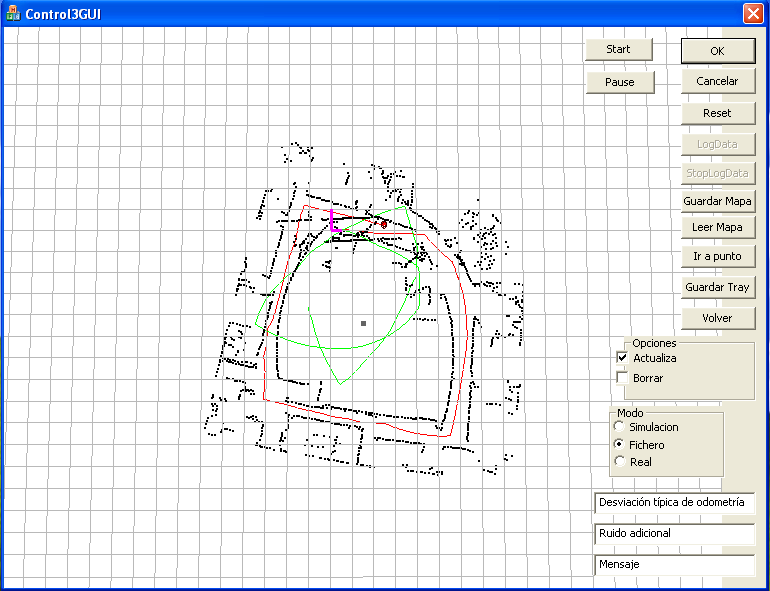
\includegraphics[scale=0.4]{intel1}\\
  \caption{Primer experimento con datos de Intel}\label{fg:intel1}
\end{figure}

En la figura \ref{fg:intel1} se puede observar que las medidas odométricas presentan un alto grado de error. Por ello, es muy probable que la varianza introducida en el filtro de Kalman para dichas medidas sea demasiado pequeña y, por lo tanto, la elaboración del mapa no sea la correcta.

El tiempo total empleado en la obtención del mapa y en el cálculo de la trayectoria corregida es: 6.8~min.

\paragraph{Prueba 2.}
En esta prueba se han utilizado los siguientes parámetros:
\begin{itemize}
  \item desviación típica del ruido de la odometría introducida en el filtro de Kalman: $\sigma_{odom} = 0.8$
  \item desviación típica del ruido de las medidas del láser: $\sigma_{med} = 0.3$
  \item ruido adicional: $\sigma_{extra} = 0$
  \item borrado de puntos dinámicos del mapa: $borrar = false$
  \item incorporación de nuevos puntos al mapa: $actualiza = true$
\end{itemize}

\paragraph{Resultados:}

\begin{figure}[h]
  \centering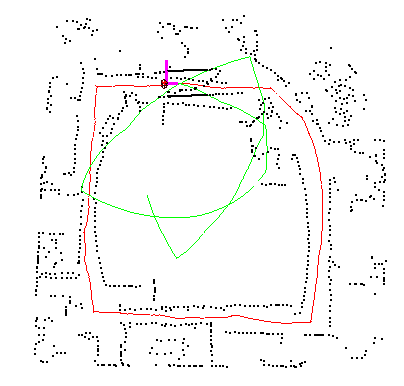
\includegraphics[scale=0.4]{intel2}\\
  \caption{Segundo experimento con datos de Intel}\label{fg:intel2}
\end{figure}

En este caso, la varianza del ruido de las medidas de odometría estimada para la utilización del filtro de Kalman resulta más adecuada y, como puede observarse, conduce a un resultado excelente a pesar de la poca calidad de los datos odométricos disponibles (figura \ref{fg:intel2}).

El tiempo total empleado en la obtención del mapa y en el cálculo de la trayectoria corregida es: 5.71~min.

\pagebreak[4]
\paragraph{Prueba 3.}
En esta prueba se han utilizado los siguientes parámetros:\nopagebreak[4]
\begin{itemize}
  \item desviación típica del ruido de la odometría introducida en el filtro de Kalman: $\sigma_{odom} = 1$
  \item desviación típica del ruido de las medidas del láser: $\sigma_{med} = 0.3$
  \item ruido adicional: $\sigma_{extra} = 0$
  \item borrado de puntos dinámicos del mapa: $borrar = true$
  \item incorporación de nuevos puntos al mapa: $actualiza = true$
\end{itemize}

\paragraph{Resultados:} 

\begin{figure}[hbtp]
  \centering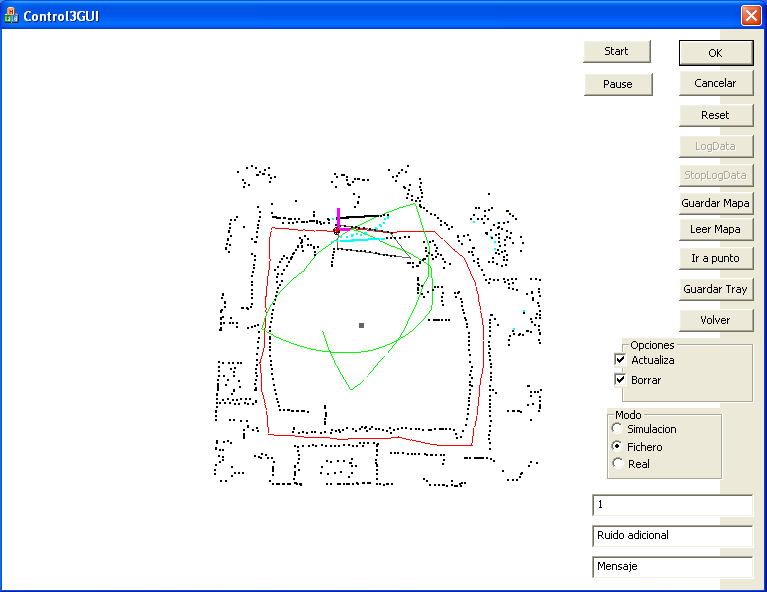
\includegraphics[scale=0.4]{intel3}\\
  \caption{Tercer experimento con datos de Intel}\label{fg:intel3}
\end{figure}

Ver figura \ref{fg:intel3}. El tiempo total empleado en la obtención del mapa y en el cálculo de la trayectoria corregida es: 6.61min.

\clearpage
\subsubsection{Utilización de datos del Museo de las Ciencias Príncipe Felipe de Valencia}

Estos datos incluyen 181 medidas del láser en cada momento. Por esta razón su procesamiento resulta más ágil que el del caso anterior. No obstante, dada la gran extensión del mapa elaborado y la exhaustiva exploración del entorno para la realización del mismo, el tiempo total consumido es notablemente superior por serlo también la duración del recorrido de toma de datos.

\paragraph{Prueba 1.}
En esta prueba se han utilizado los siguientes parámetros:
\begin{itemize}
  \item desviación típica del ruido de la odometría introducida en el filtro de Kalman: $\sigma_{odom} = 0.9$
  \item desviación típica del ruido de las medidas del láser: $\sigma_{med} = 0.3$
  \item ruido adicional: $\sigma_{extra} = 0$
  \item borrado de puntos dinámicos del mapa: $borrar = false$
  \item incorporación de nuevos puntos al mapa: $actualiza = true$
\end{itemize}


\paragraph{Resultados:} 
\begin{figure}[h]
  \centering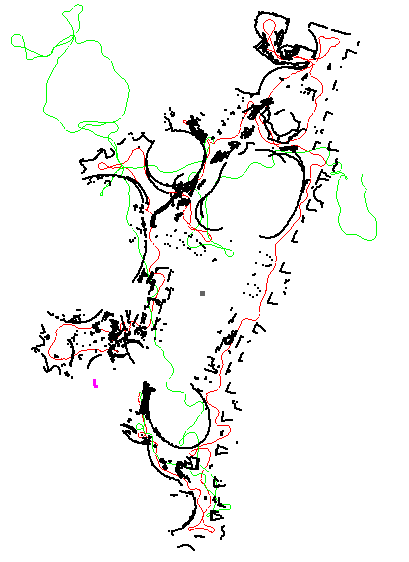
\includegraphics[scale=0.5]{val3}\\
  \caption{Primer experimento con datos del Museo de las Ciencias Príncipe Felipe de Valencia}\label{fg:val3}
\end{figure}

Figura \ref{fg:val3}. El tiempo total empleado en la obtención del mapa y en el cálculo de la trayectoria corregida es: 26.54~min.


\paragraph{Prueba 2.} En esta prueba se han utilizado los siguientes parámetros:
\begin{itemize}
  \item desviación típica del ruido de la odometría introducida en el filtro de Kalman: $\sigma_{odom} = 0.9$
  \item desviación típica del ruido de las medidas del láser: $\sigma_{med} = 0.3$
  \item ruido adicional: $\sigma_{extra} = 0$
  \item borrado de puntos dinámicos del mapa: $borrar = true$
  \item incorporación de nuevos puntos al mapa: $actualiza = true$
\end{itemize}

\paragraph{Resultados:}
\begin{figure}[h]
  % Requires \usepackage{graphicx}
  \centering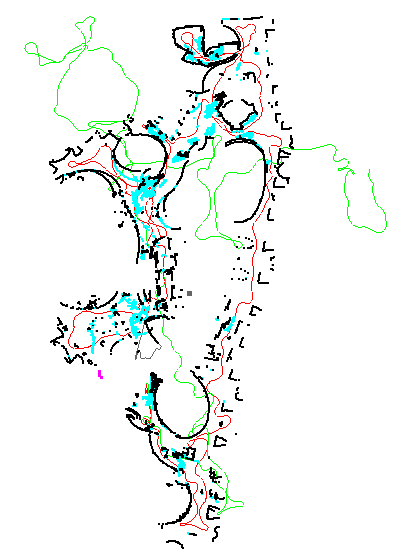
\includegraphics[scale=0.4]{val2}\\
  \caption{Segundo experimento con datos del Museo de las Ciencias Príncipe Felipe de Valencia}\label{fg:val2}
\end{figure}

Figura \ref{fg:val2}.El tiempo total empleado en la obtención del mapa y en el cálculo de la trayectoria corregida es: 36.01~min.

Como puede observarse, la presencia de personas en el museo afecta a la construcción del mapa y a la localización. Esto puede corregirse mediante el borrado de puntos del mapa, con lo que se logra un resultado realmente bueno. A pesar de la gran longitud de la trayectoria seguida, con el correspondiente incremento de errores en las medidas de los encoders, el sistema mantiene una correcta estimación de la posición del robot hasta el final del recorrido efectuado.

\subsection{Pruebas en modo \emph{real}}
Como ya se ha mencionado, en estas pruebas se ha trabajado con el robot móvil Urbano. A continuación se muestran algunos de los mapas obtenidos en el laboratorio del departamento llevando al robot en modo teleoperado. Los mapas realizados mediante movimiento planificado, empleando el control diseñado, se incluyen en el capítulo \ref{ch:integracion}.

% -*- coding: utf-8 -*-

\chapter[Control de movimiento]
{Control de movimiento, planificación de trayectorias y control reactivo}%
\label{ch:movimiento}

\section{Control de movimiento}\label{control}

Las variables sobre las que se actúa para controlar el movimiento del robot son las velocidades de avance y giro. Sus sentidos son los indicados en la figura \ref{fg:velocidades}:

\begin{figure}[hbt]
  % Requires \usepackage{graphicx}
  \centering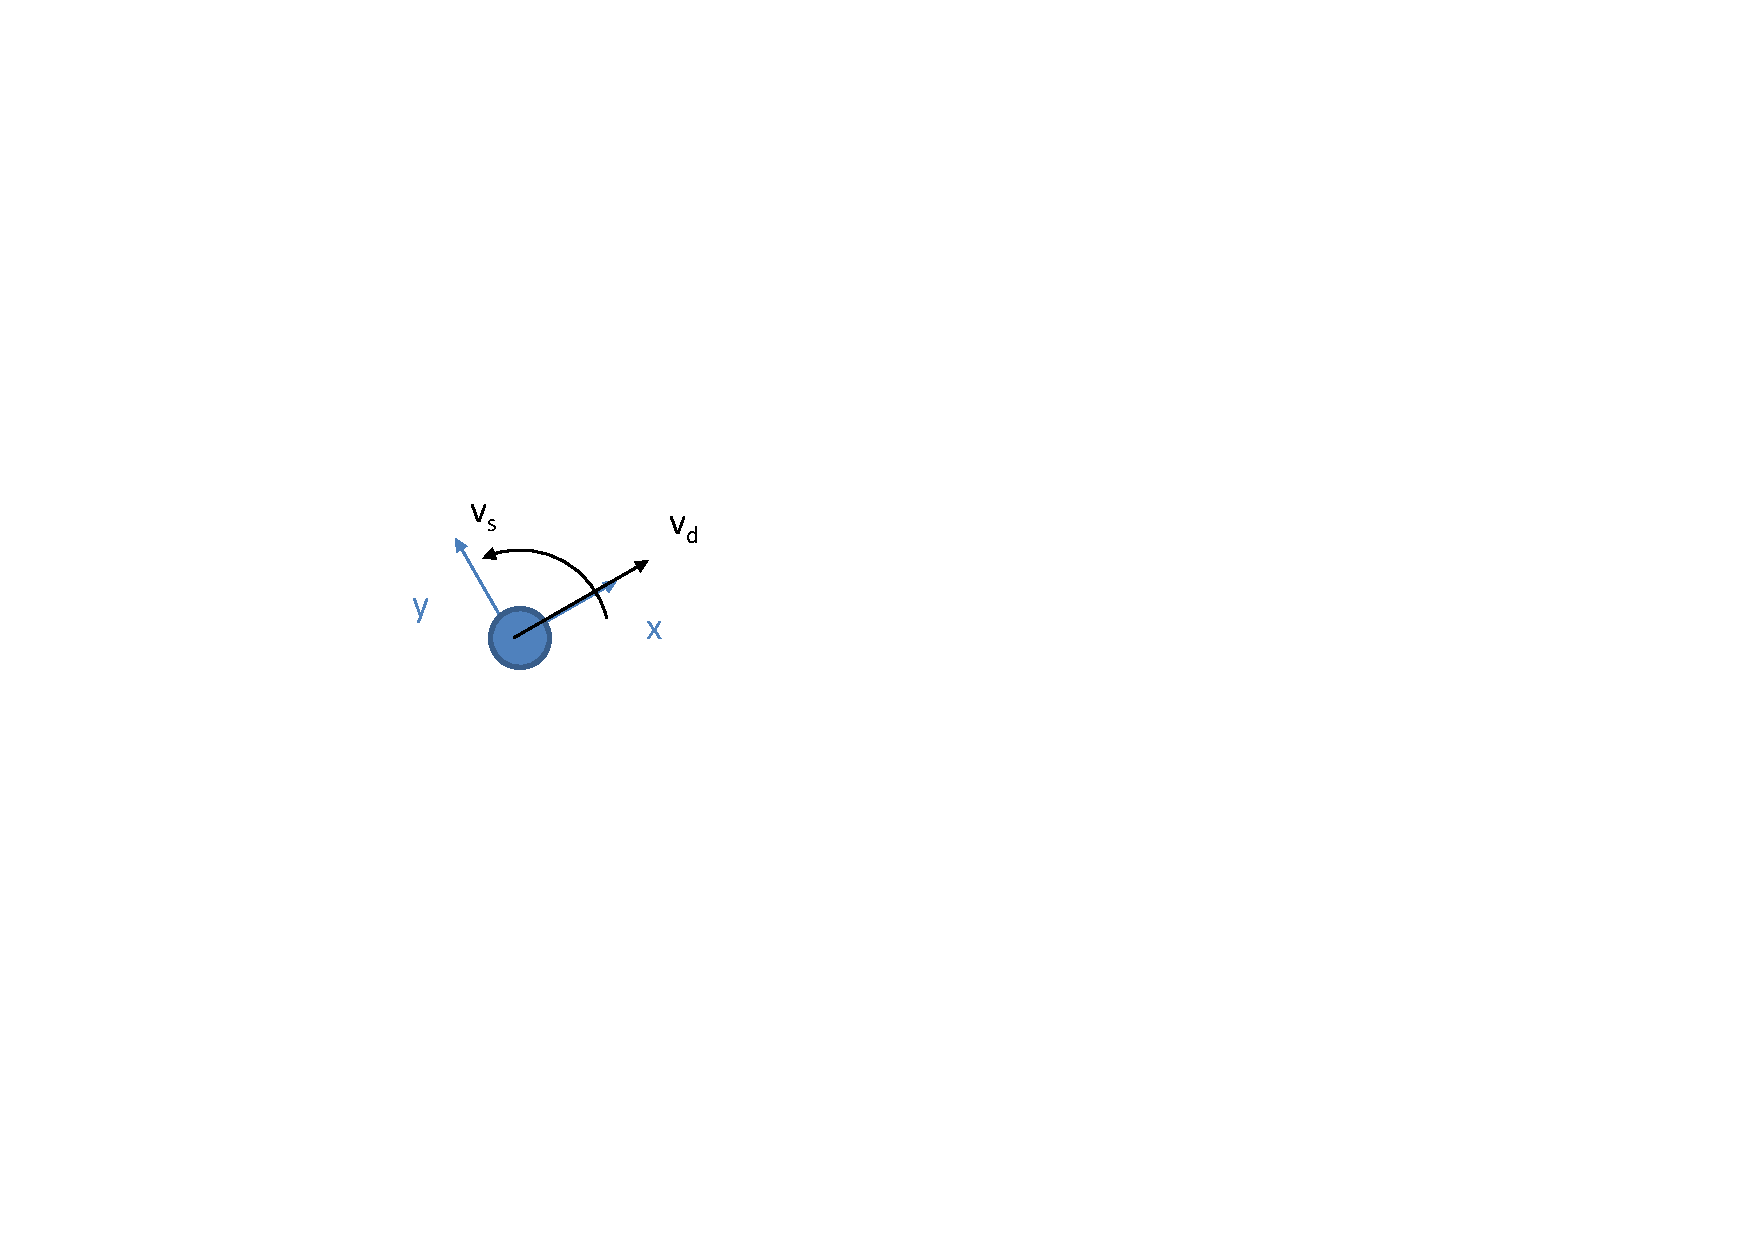
\includegraphics[scale=0.7]{velocidades}\\
  \caption{Velocidad de avance y giro en el sistema de referencia local del robot}\label{fg:velocidades}
\end{figure}


La medida de ángulos se realiza en todo momento en el intervalo [$-\pi$,$\pi$]. Para efectuar la conversión a este rango se utiliza la función \prog{AngRango}.

Como se expuso en el capítulo \ref{ch:estado}, resulta conveniente utilizar un regulador con realimentación que emplee información sobre la posición del robot en cada instante para obtener unos valores de velocidad que permitan llegar al objetivo dado.

Para que el robot se traslade mirando de frente la mayor parte del tiempo, se busca minimizar la diferencia entre su orientación y la del vector que lo une con el punto de destino. Al mismo tiempo el robot deberá irse acercando a dicho punto de destino.

\begin{figure}[bt]
  % Requires \usepackage{graphicx}
  \centering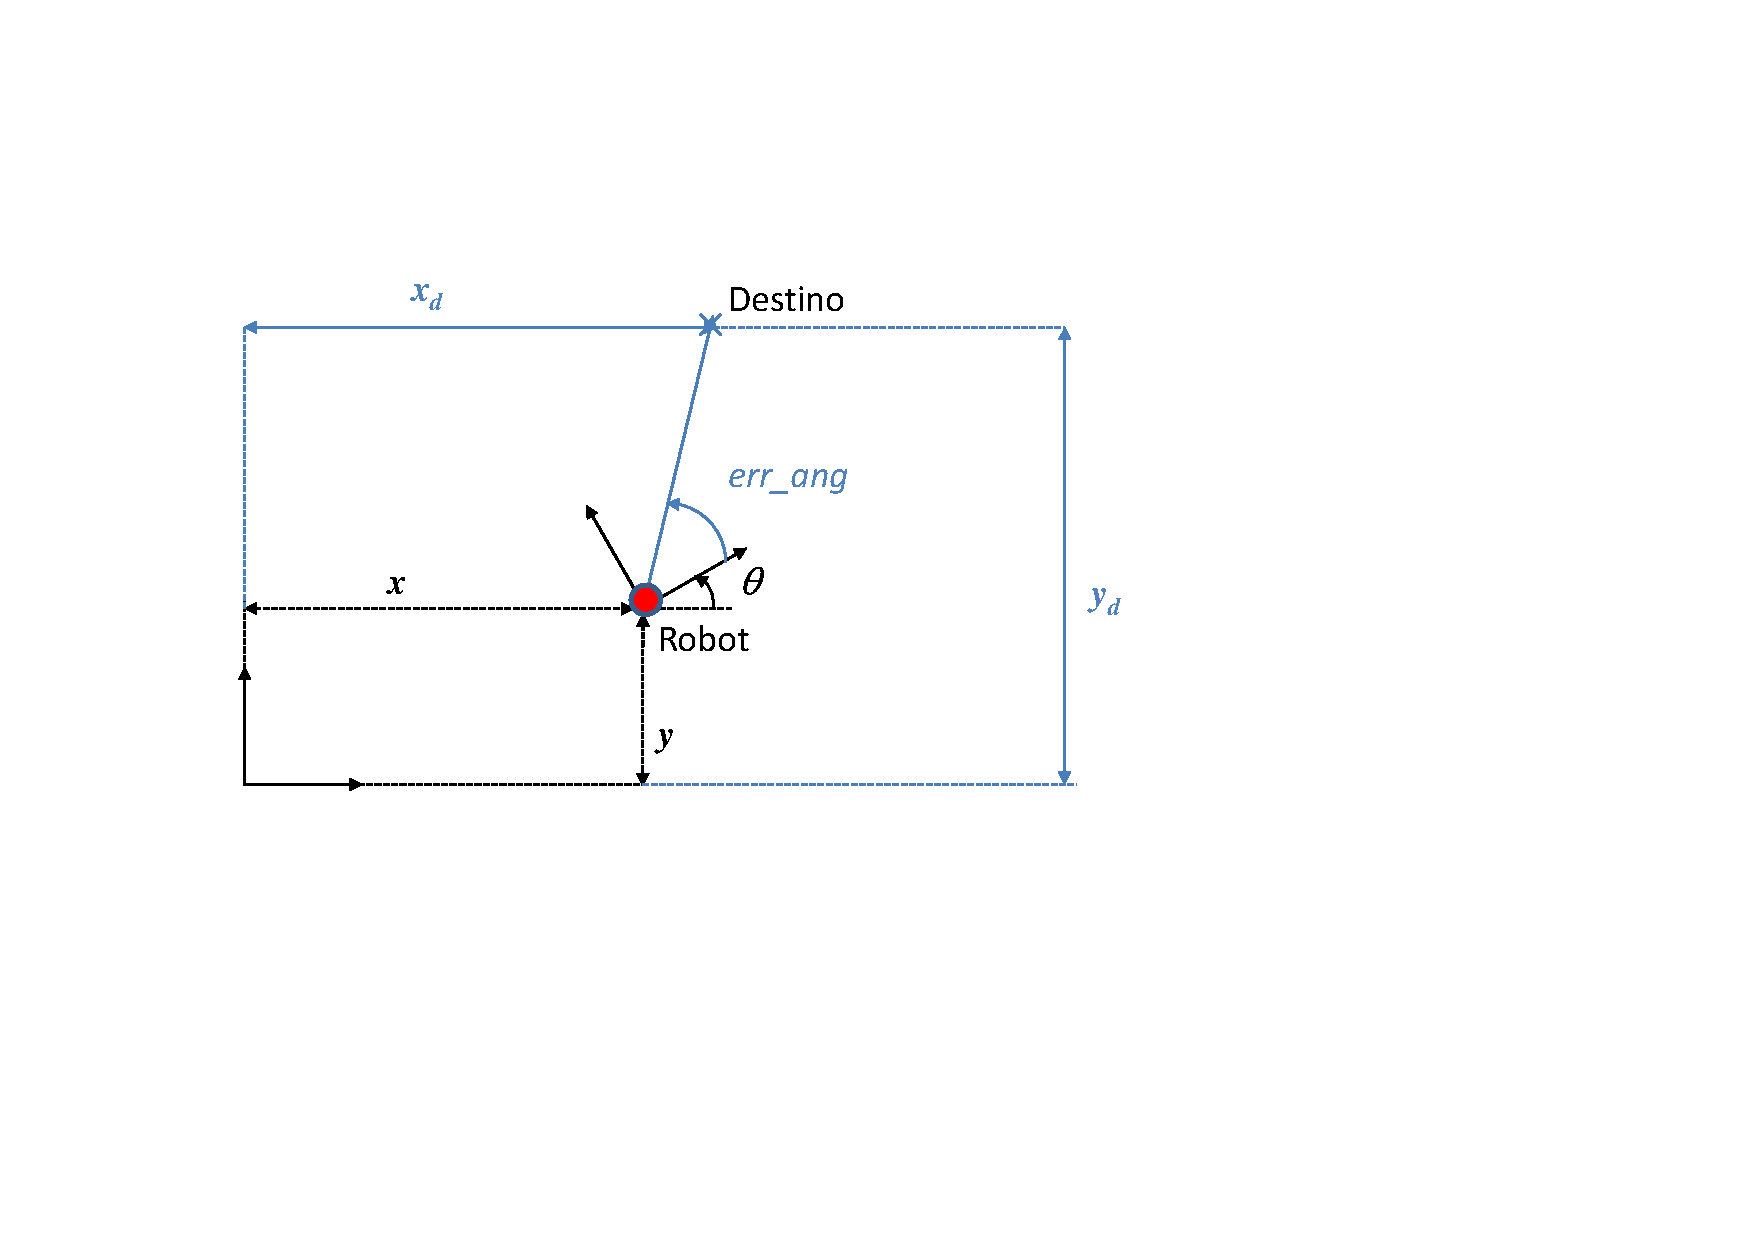
\includegraphics[scale=0.6]{err_ang}\\
  \caption{Control de la orientación del robot}\label{fg:err_ang}
\end{figure}

\begin{figure}[bt]
  % Requires \usepackage{graphicx}
  \centering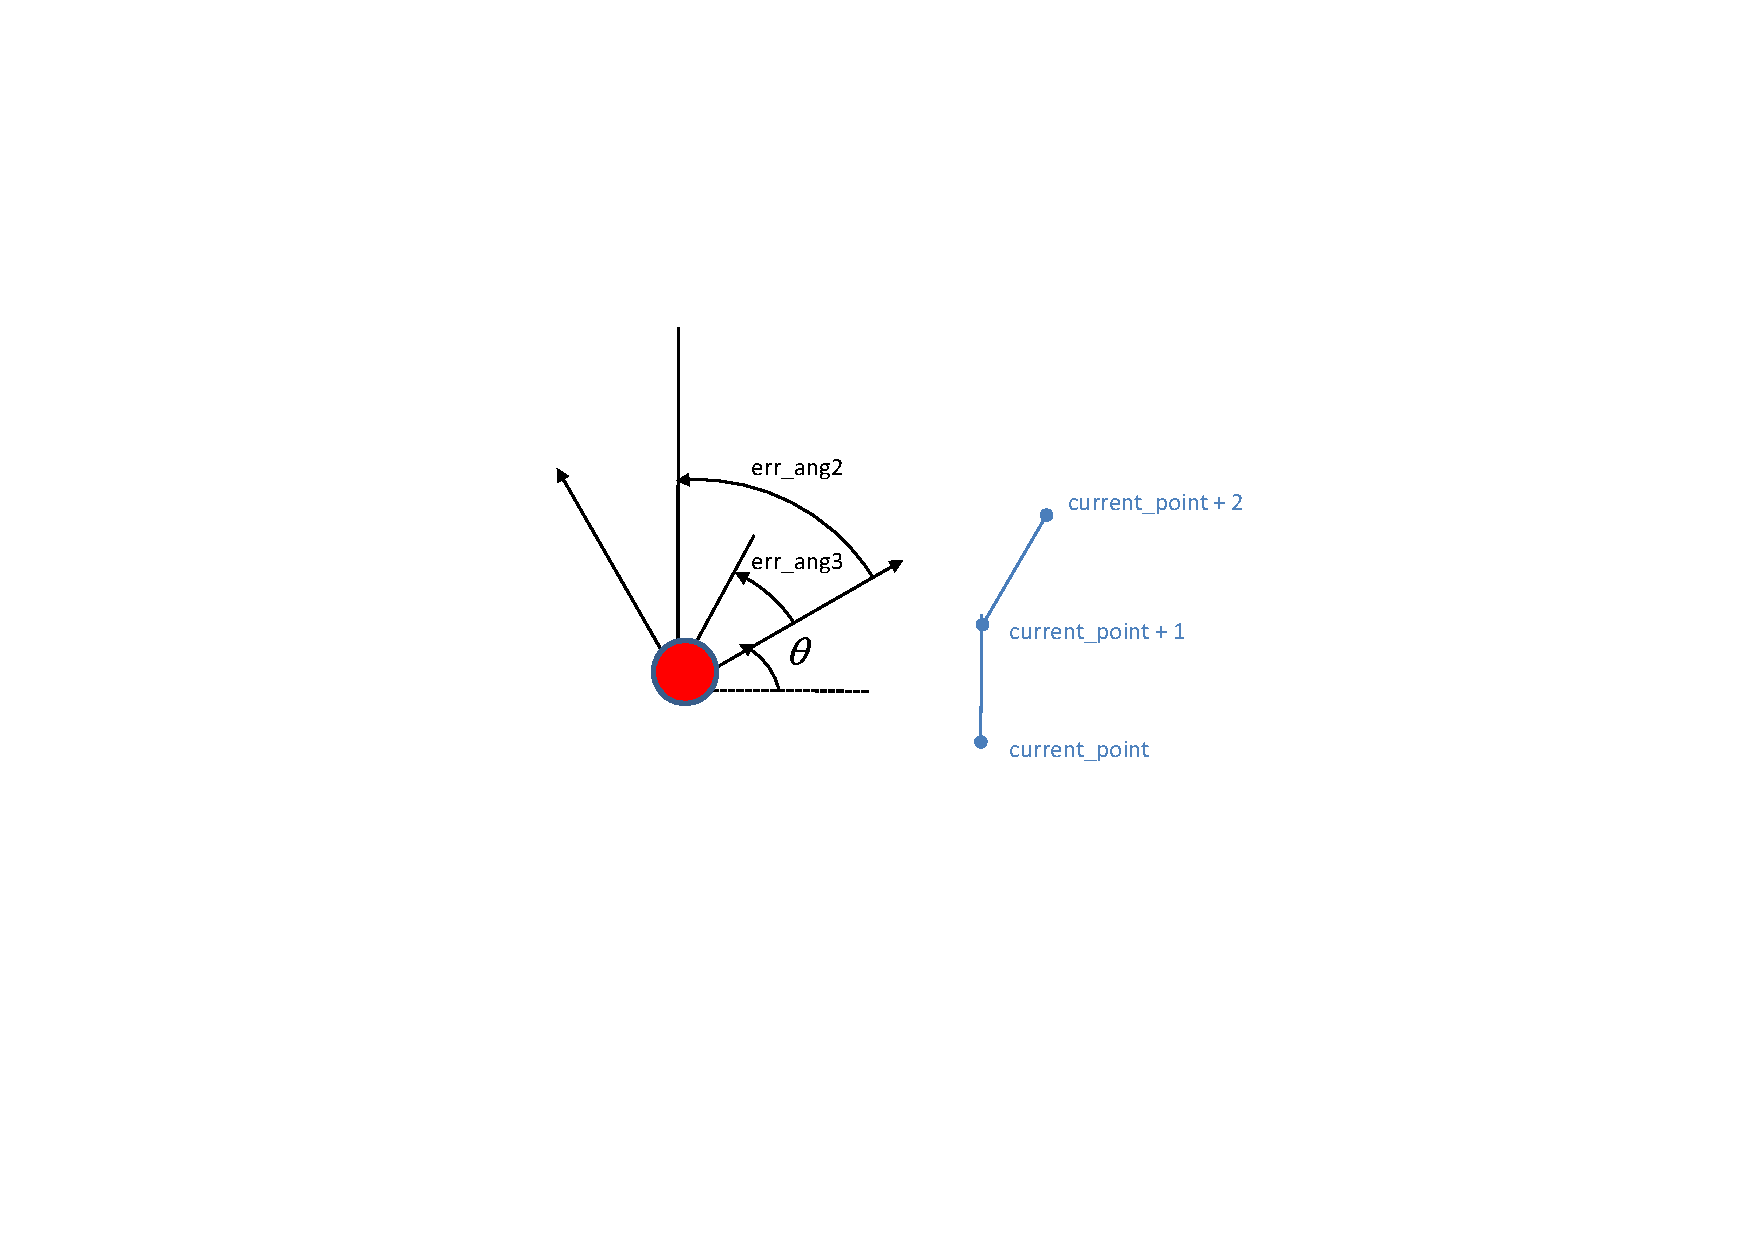
\includegraphics[scale=0.5]{err_ang23}\\
  \caption{Nuevos errores incorporados al regulador}\label{fg:err_ang23}
\end{figure} 

Como puede verse en la figura \ref{fg:err_ang}, el ángulo resultante de esa diferencia de orientaciones se llamará \prog{err\_ang}. En función de su valor se distinguen cuatro casos principales en los cuales se utilizaron en una primera aproximación las ganancias indicadas en el cuadro \ref{vel1}, donde todas las magnitudes están expresadas en el Sistema Internacional salvo cuando se especifica lo contrario.

\begin{table}[hbt]
\begin{center}
\caption{Regulador inicial para el control de movimiento} \label{vel1}

\vspace{5mm}

\begin{tabular}{ll}
\hline\hline
170º$<err\_ang(º)$ \\ \hline
Urbano:      &  Pioneer:   \\
        $v_{d}=0$                   & $v_{d}=0$\\
        $v_{s}=30err\_ang$  & $v_{s}=0.65err\_ang$ \\
\hline
  45º$<err\_ang(º)<$170º \\ \hline
Urbano:  & Pioneer:\\
        $v_{d}=2$                  & $v_{d}=0.025$\\
        $v_{s}=40err\_ang$ & $v_{s}=0.7err\_ang$\\
\hline
15º$<err\_ang(º)<$45º \\ \hline
Urbano:      &  Pioneer:   \\
        $v_{d}=6$                  & $v_{d}=0.1$\\
        $v_{s}=34err\_ang$ & $v_{s}=0.7err\_ang$ \\
\hline
$err\_ang(º)<$15º \\ \hline
Urbano:  & Pioneer: \\
        $v_{d}=10$                & $v_{d}=0.4$\\
        $v_{s}=26err\_ang$ & $v_{s}=0.6err\_ang$\\
\hline\hline
\end{tabular}
\end{center}
\end{table}

Al aumentar la duración del ciclo de tareas cuando se utiliza el robot real Urbano, los comandos de velocidad enviados de acuerdo con el cuadro a \ref{vel1} llegaban con retraso y el robot daba algunos bandazos. Para solucionar este problema se modificó el regulador de forma que se contemplara también la orientación de la trayectoria en el tramo en que se encuentra el robot en cada instante y la orientación en el tramos siguiente, a modo de control predictivo. Los nuevos ángulos sobre los que también se actúa se denominarán \prog{err\_ang2} y \prog{err\_ang3}, respectivamente, y se muestran en la figura \ref{fg:err_ang23}.
 
La acción de control resultante es una combinación lineal de las acciones sobre estos tres ángulos. Se ha utilizado un peso de 0.3 para regular \prog{err\_ang}, un peso de 0.2 para regular \prog{err\_ang2} y un peso de 0.5 para regular \prog{err\_ang3}. El regulador final obtenido utiliza los valores y ganancias que aparecen en el cuadro \ref{vel2}, donde de nuevo las magnitudes se expresan en el S.I. a no ser que se especifique lo contrario. $p1$, $p2$ y $p3$ son los pesos indicados (0.3, 0.2 y 0.5).
Con el robot Pioneer los pesos son los mismos y se mantienen las ganancias del cuadro \ref{vel1}.

\begin{table}[hbt]
\begin{center}
\caption{Regulador para el control de movimiento}
\label{vel2}

\vspace{5mm}

\begin{tabular}{ll}
\hline\hline
160º$<err\_ang(º)$ \\ \hline
Urbano:\\
$v_{d}=0$ \\
$v_{s}=30err\_ang$\\
\hline
  45º$<err\_ang(º)<$160º \\ \hline
Urbano:\\
   $v_{d}=3$ \\
  $v_{s}=p1\times3oerr\_ang + p2\times3oerr\_ang2 + p3\times3oerr\_ang3$ \\
\hline
15º$<err\_ang(º)<$45º \\ \hline
Urbano:\\
$v_{d}=5$ \\
$v_{s}=p1\times26err\_ang + p2\times26err\_ang2 + p3\times26err\_ang3$\\
\hline
$err\_ang(º)<$15º \\ \hline
Urbano: \\
$v_{d}=10$\\
 $v_{s}=p1\times20err\_ang + p2\times26err\_ang2 + p3\times26err\_ang3$\\
\hline\hline
\end{tabular}
\end{center}
\end{table}

El sistema funciona como una máquina de estados. Cuando el robot está lo suficientemente cerca del punto de destino se considera que ha llegado y se establece como destino el siguiente punto de la trayectoria definida. Cuando la distancia al último punto de la misma es menor que 0.5m, actúa un regulador proporcional para que la velocidad de avance del robot vaya disminuyendo gradualmente a medida que se aproxima el final de su recorrido.

Si por algún motivo el robot se halla separado de la trayectoria calculada entre dos puntos, este controlador lo llevaría directamente hacia el punto de destino en línea recta. Esto podría ocasionar el choque con algún obstáculo. Por ello, se utiliza también un regulador que hace que el robot se acerque a la trayectoria definida antes de dirigirse hacia el siguiente punto a alcanzar. Esta situación se muestra en la figura \ref{fg:reg}.

\begin{figure}[h]
  % Requires \usepackage{graphicx}
  \centering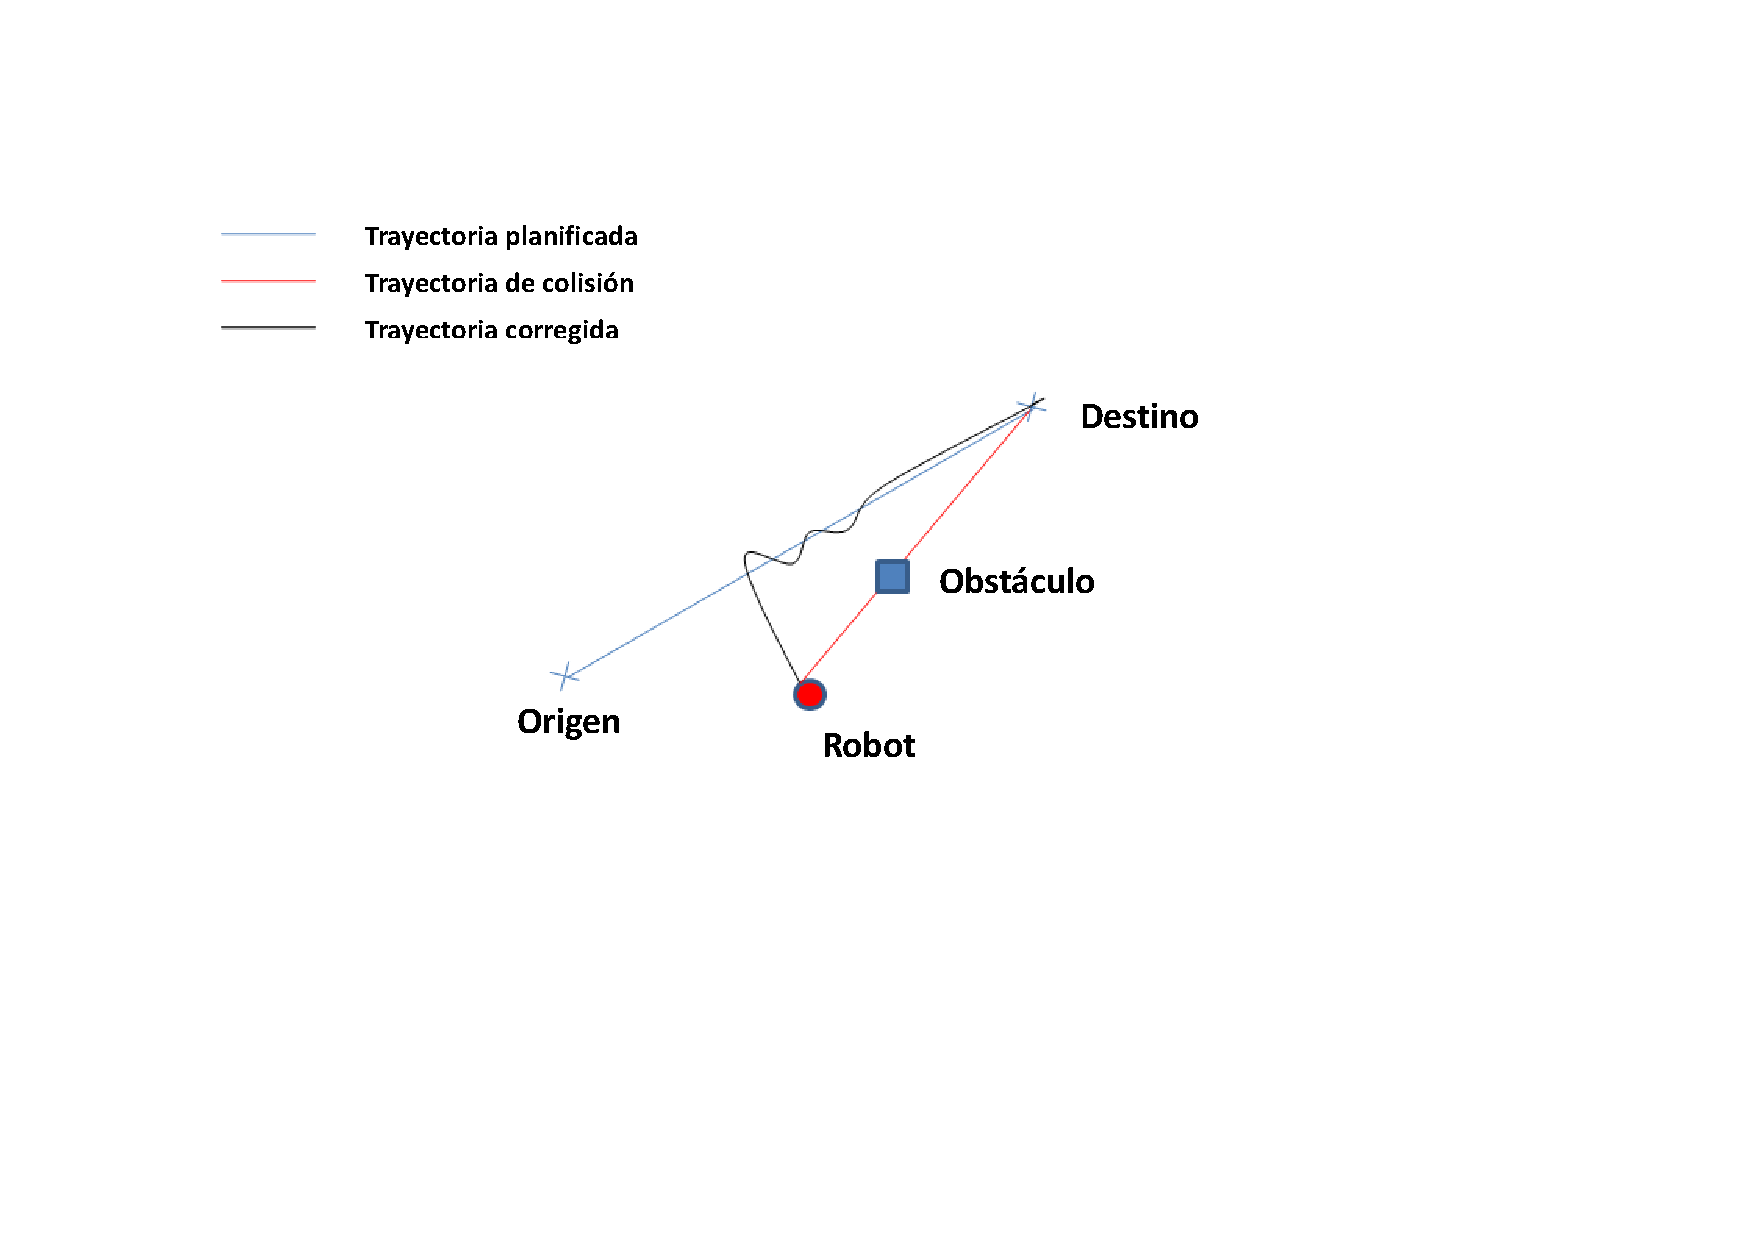
\includegraphics[scale=0.6]{reg}\\
  \caption{Diferentes trayectorias entre dos puntos}\label{fg:reg}
\end{figure}

El algoritmo empleado en este caso requiere medir en primer lugar la distancia de la posición del robot a la recta que une los dos puntos de la trayectoria entre los que se encuentra. Esta distancia tendrá signo positivo o negativo dependiendo de a qué lado de la trayectoria se encuentre el robot (figura \ref{fg:dist2tray}).

\begin{figure}[h]
  % Requires \usepackage{graphicx}
  \centering{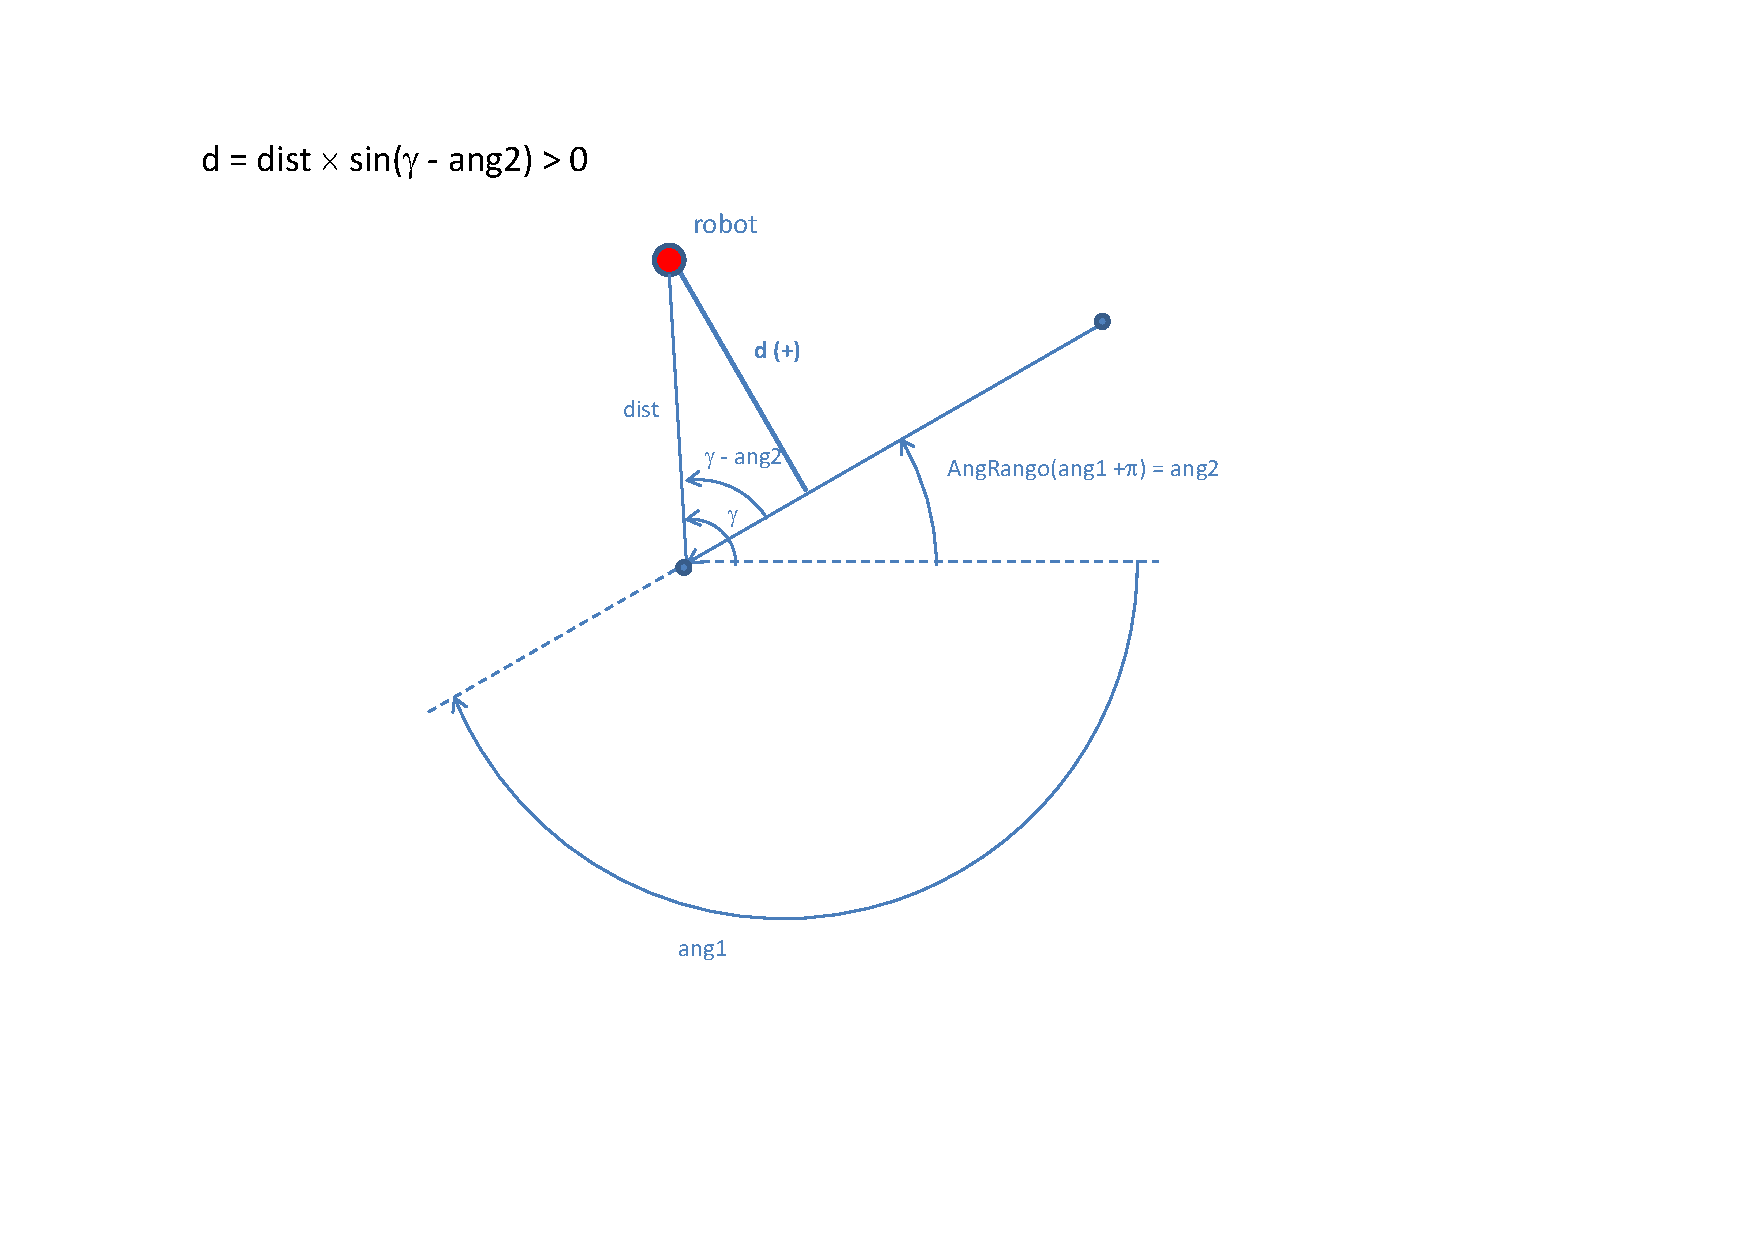
\includegraphics[scale=0.6]{dist2tray}
  \vspace{0.2cm}
   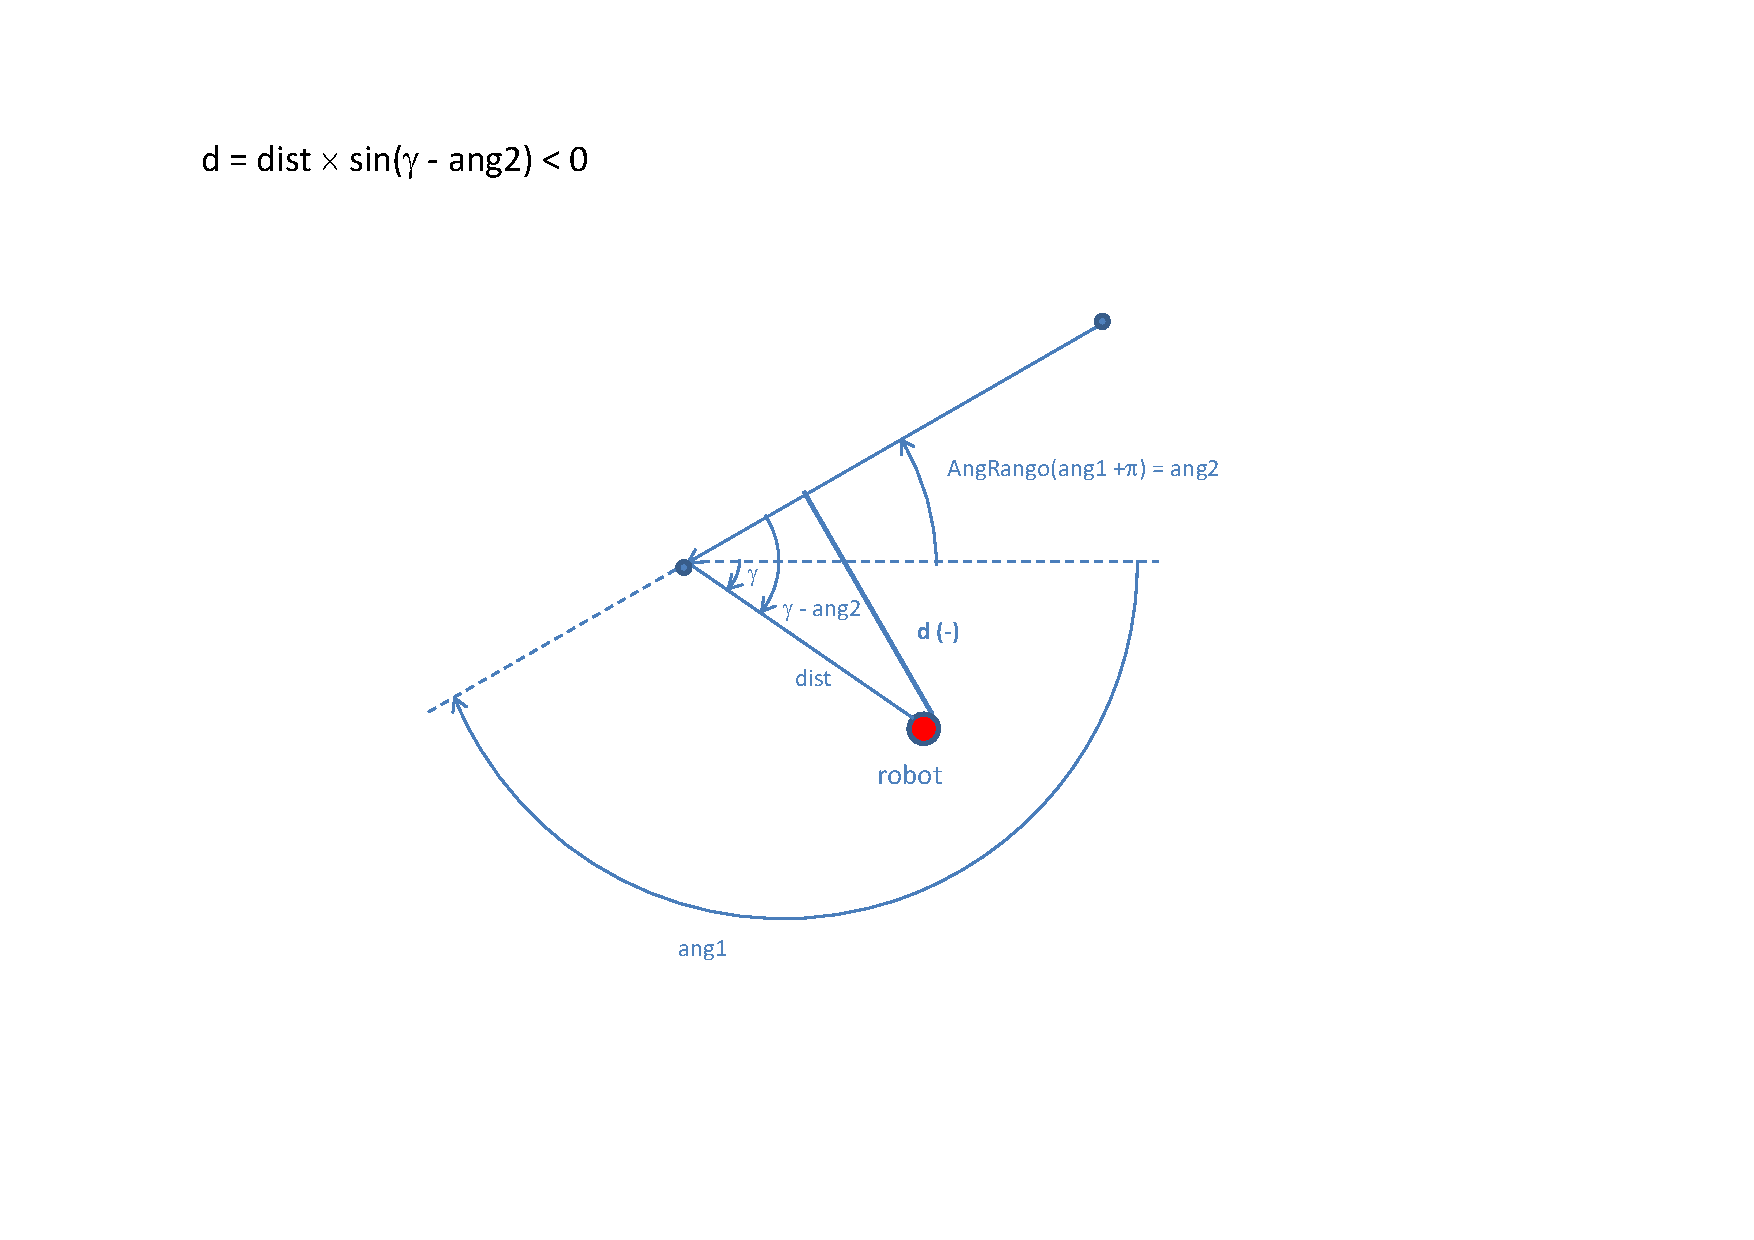
\includegraphics[scale=0.6]{dist2tray2}}  \\
  \caption{ Medida de la distancia del robot al segmento de trayectoria en el que se halla}\label{fg:dist2tray}
\end{figure}

\clearpage

Si el robot está más lejos de la trayectoria que lo establecido por un cierto valor límite, se realizará un control que tienda a dirigirlo perpendicularmente hacia la misma. Para ello se utilizan unos valores de ganancia muy similares a los indicados en la tabla anterior, pero el ángulo que se mide es aquél que separa la orientación del robot con la que debería tener para acercarse perpendicularmente al segmento de trayectoria correspondiente. El modo en que se calcula este ángulo en dos casos en que el robot está situado a un lado u otro de un mismo segmento se muestra en la figura \ref{fg:regu}.

\begin{figure}[hbt]
  % Requires \usepackage{graphicx}
  \centering{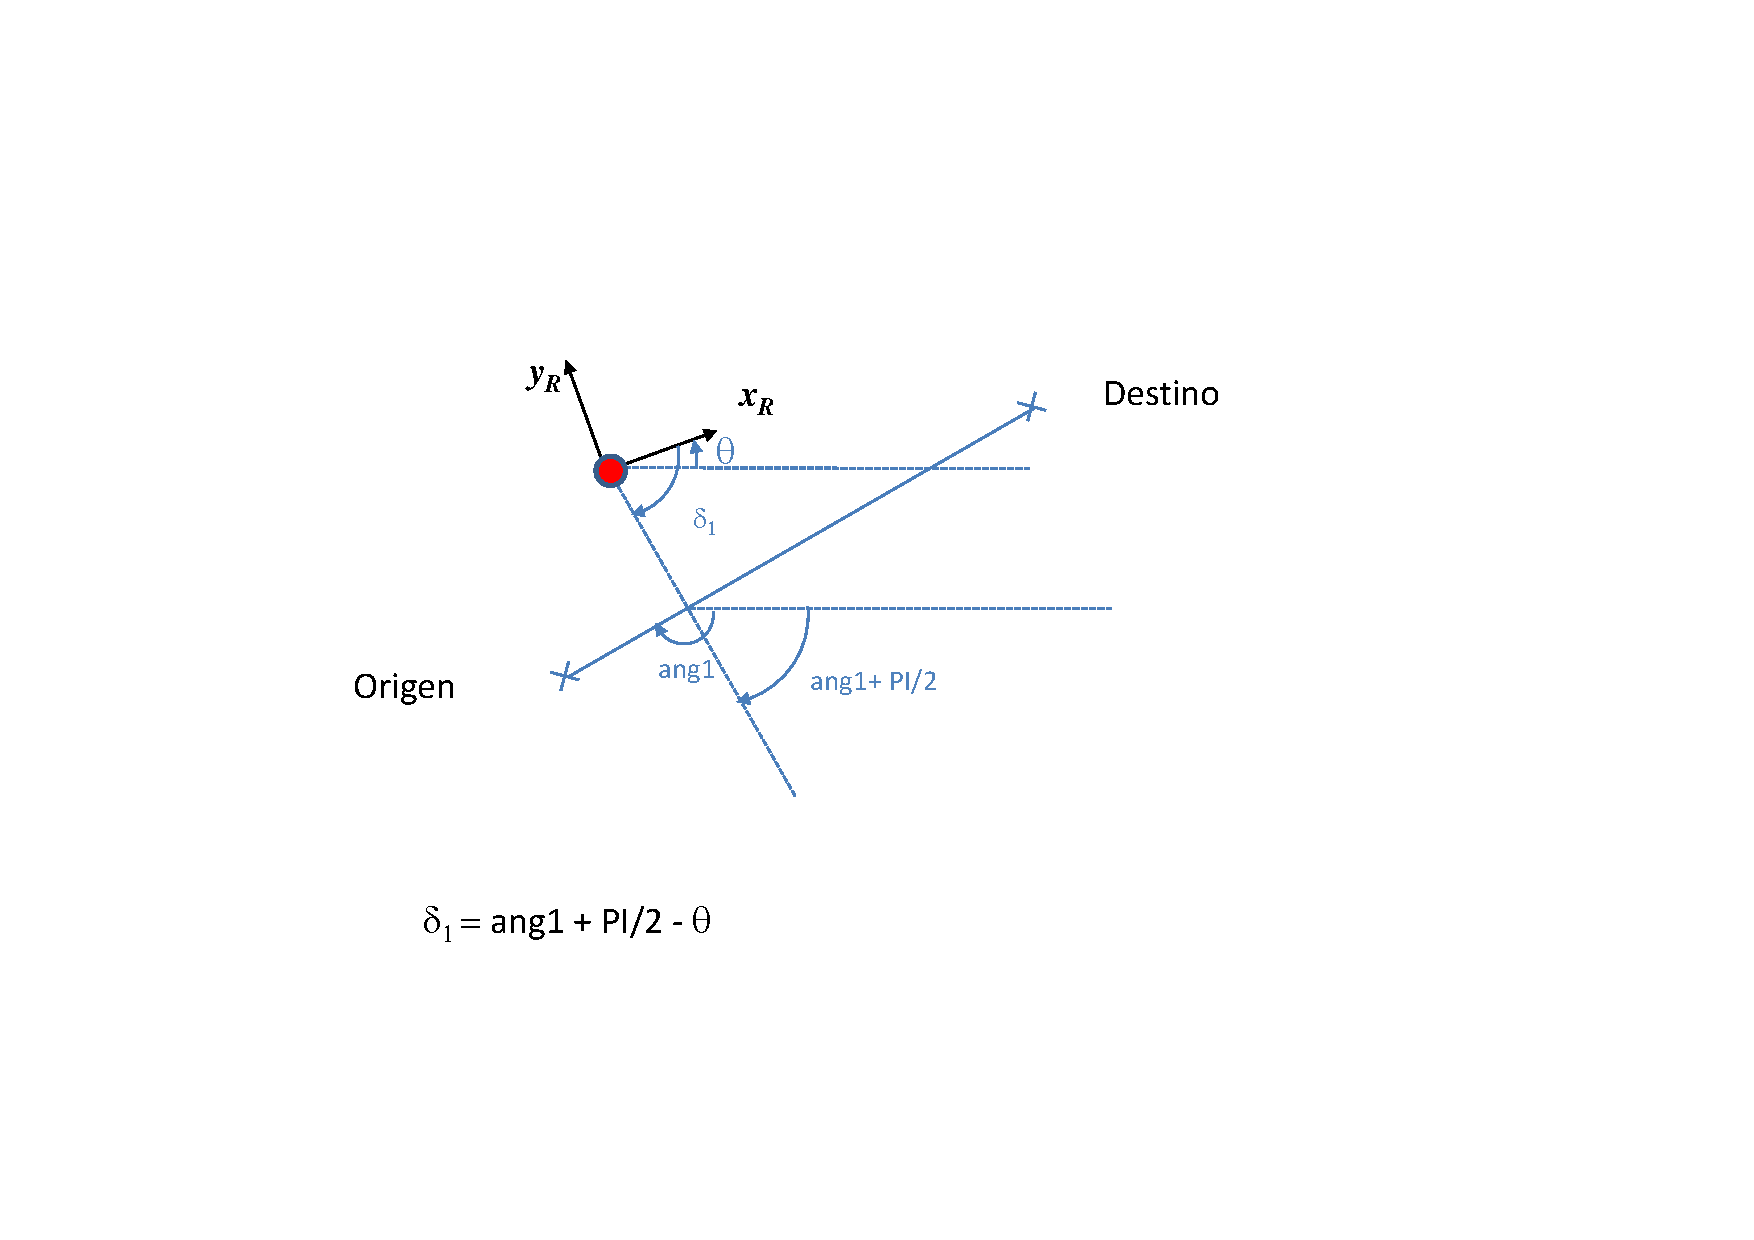
\includegraphics[scale=0.5]{regu1}
  \vspace{0.5cm} 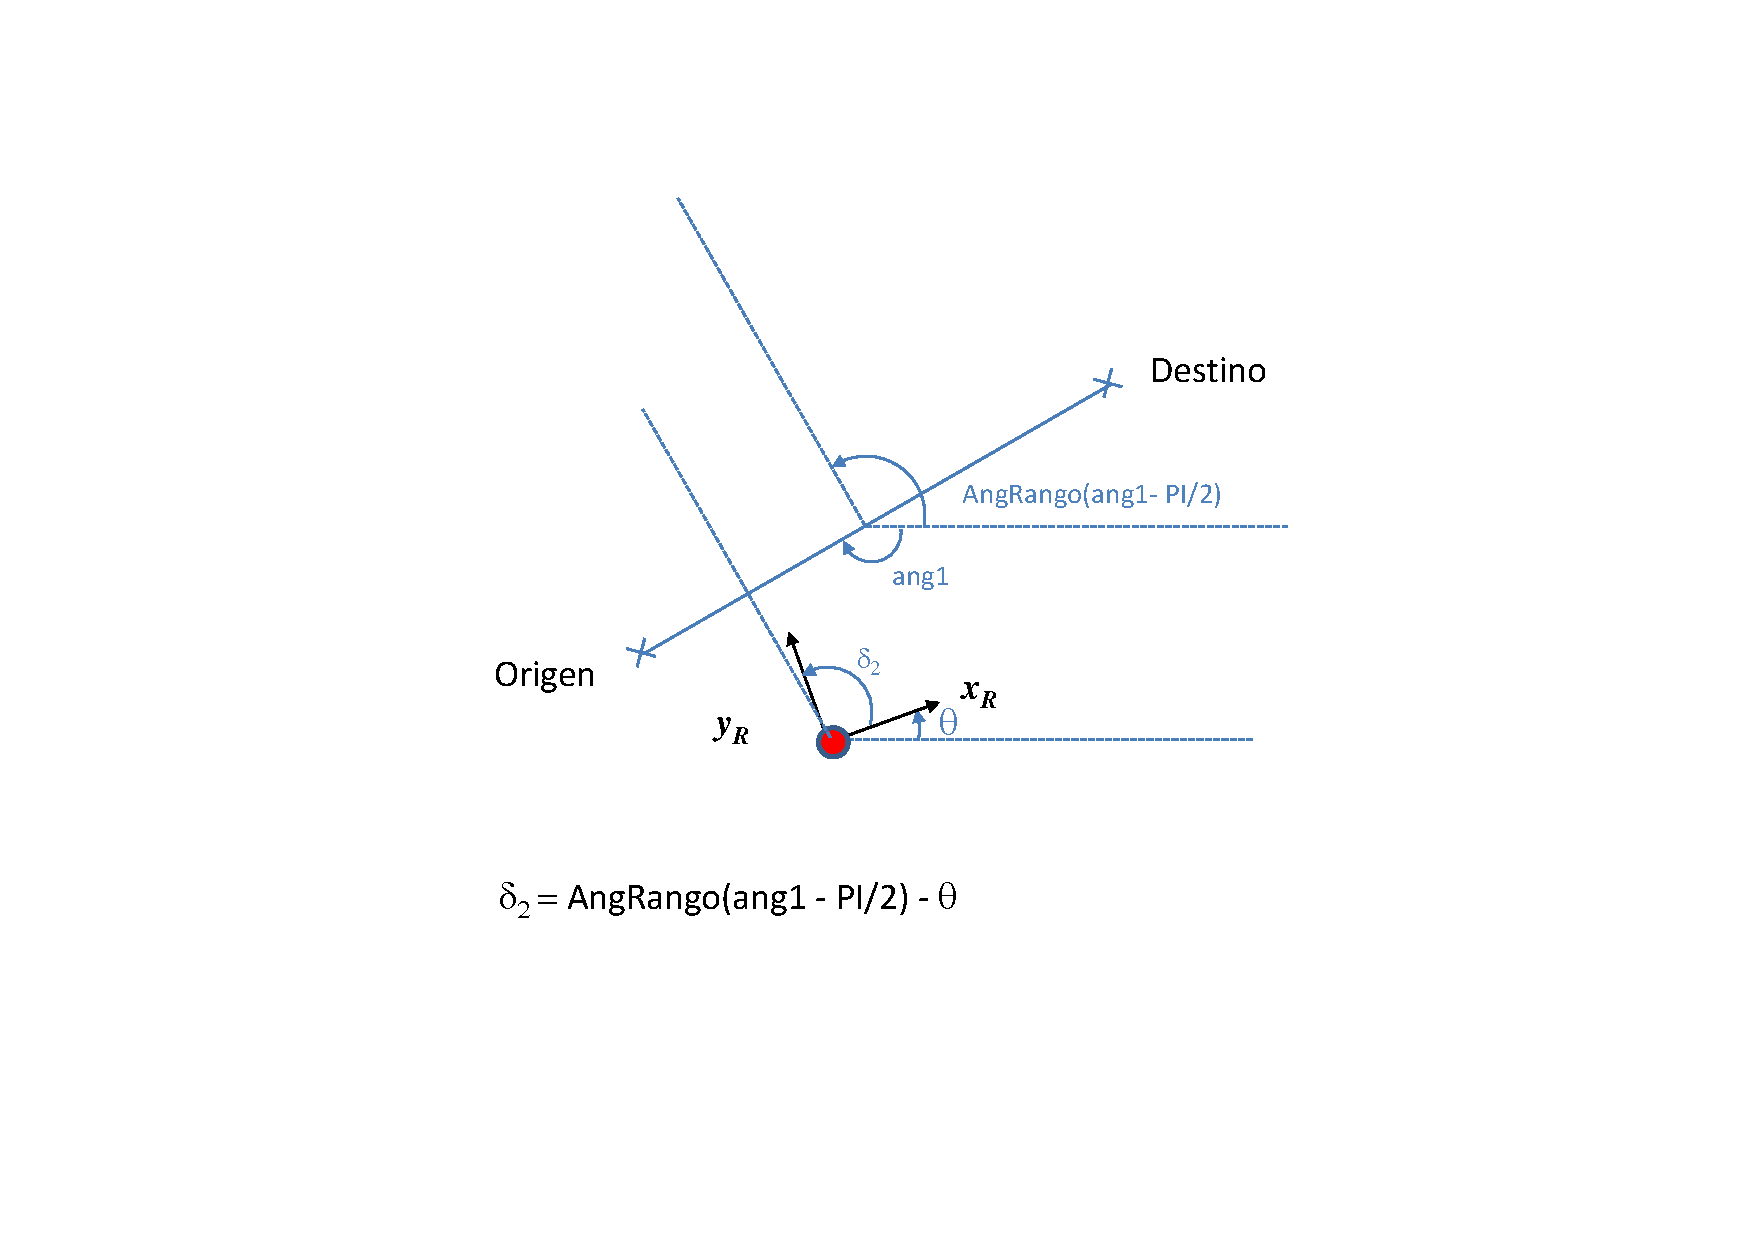
\includegraphics[scale=0.5]{regu2}}  \\
  \caption{Ángulo a regular para que el robot se aproxime a la trayectoria definida en dos casos diferentes}\label{fg:regu}
\end{figure}

\clearpage
Otro aspecto que se tiene en cuenta en el diseño del regulador es el hecho de que el robot pueda pasarse de algún punto de la trayectoria al hallarse muy próximos unos puntos a otros y ser la velocidad alta. En ese caso resultaría absurdo que el robot regresara a dicho punto para seguir la secuencia exacta. Es más conveniente que se dirija hacia aquél que, estando relativamente cerca del destino teórico, sea más cercano al robot. Lo mismo ocurre si la tolerancia que determina si se ha llegado o no a un punto es excesivamente pequeña. Para ello, cada vez que se van a calcular unas nuevas velocidades se busca si en la trayectoria hay algún punto entre los cinco siguientes al punto de destino que se encuentre a menos distancia de la posición del robot que éste.

\section{Planificación de trayectorias}\label{tray}

Como se ha visto en la sección anterior, el control de movimiento del robot precisa disponer de un conjunto de puntos de paso que se vayan definiendo como destinos sucesivos, conformando la trayectoria que ha de seguirse. El alcance de este proyecto no incluye la generación automática de dichos puntos de paso a partir de un destino final dentro de un mapa. Lo que puede hacerse es seleccionar la serie de puntos que determina la trayectoria mediante uso del ratón sobre la interfaz gráfica en la que se ve un mapa o parte de uno. Otra posibilidad para obtener los puntos de la trayectoria consiste en llevar el robot hacia un sitio en modo teleoperado e ir guardando su posición cada vez que recorre una cierta distancia de forma que puede regresar al punto del que partió de manera autónoma.

Cuando los puntos que dan lugar a la trayectoria están bastante separados conviene suavizar los cambios de dirección en la misma. El algoritmo utilizado para ello se explica a continuación.

Mientras sea posible, para cada punto de la trayectoria se toma el siguiente a él como base o punto intermedio a suprimir en caso necesario. Se definen dos vectores que van desde la base hasta el punto anterior y hasta el punto siguiente a ella, respectivamente, y se mide el ángulo que los separa. Si este ángulo, que llamaremos erro\_ang, es menor que 20º o superior a 160º no ha de redondearse la trayectoria; simplemente se pasa al siguiente de sus puntos. En caso contrario se halla su bisectriz para situar sobre ella el centro del arco de circunferencia que servirá para suavizar la trayectoria en el punto base. A partir del centro se irán determinando puntos de forma que su distancia a él sea igual al radio y que queden uniformemente repartidos sobre un arco tangente a los dos segmentos de trayectoria que se unen. El cálculo de los ángulos que permiten calcular las coordenadas de los puntos del arco se basa en un ángulo auxiliar definido como \prog{alfa\_ref} = \prog{AngRango}$(\pi - ang\_bis)$ y es diferente según \prog{erro\_ang} sea positivo o negativo, dado que esto condiciona el sentido en que deben ir creciendo dichos ángulos.

\begin{figure}[bt]
  % Requires \usepackage{graphicx}
  \centering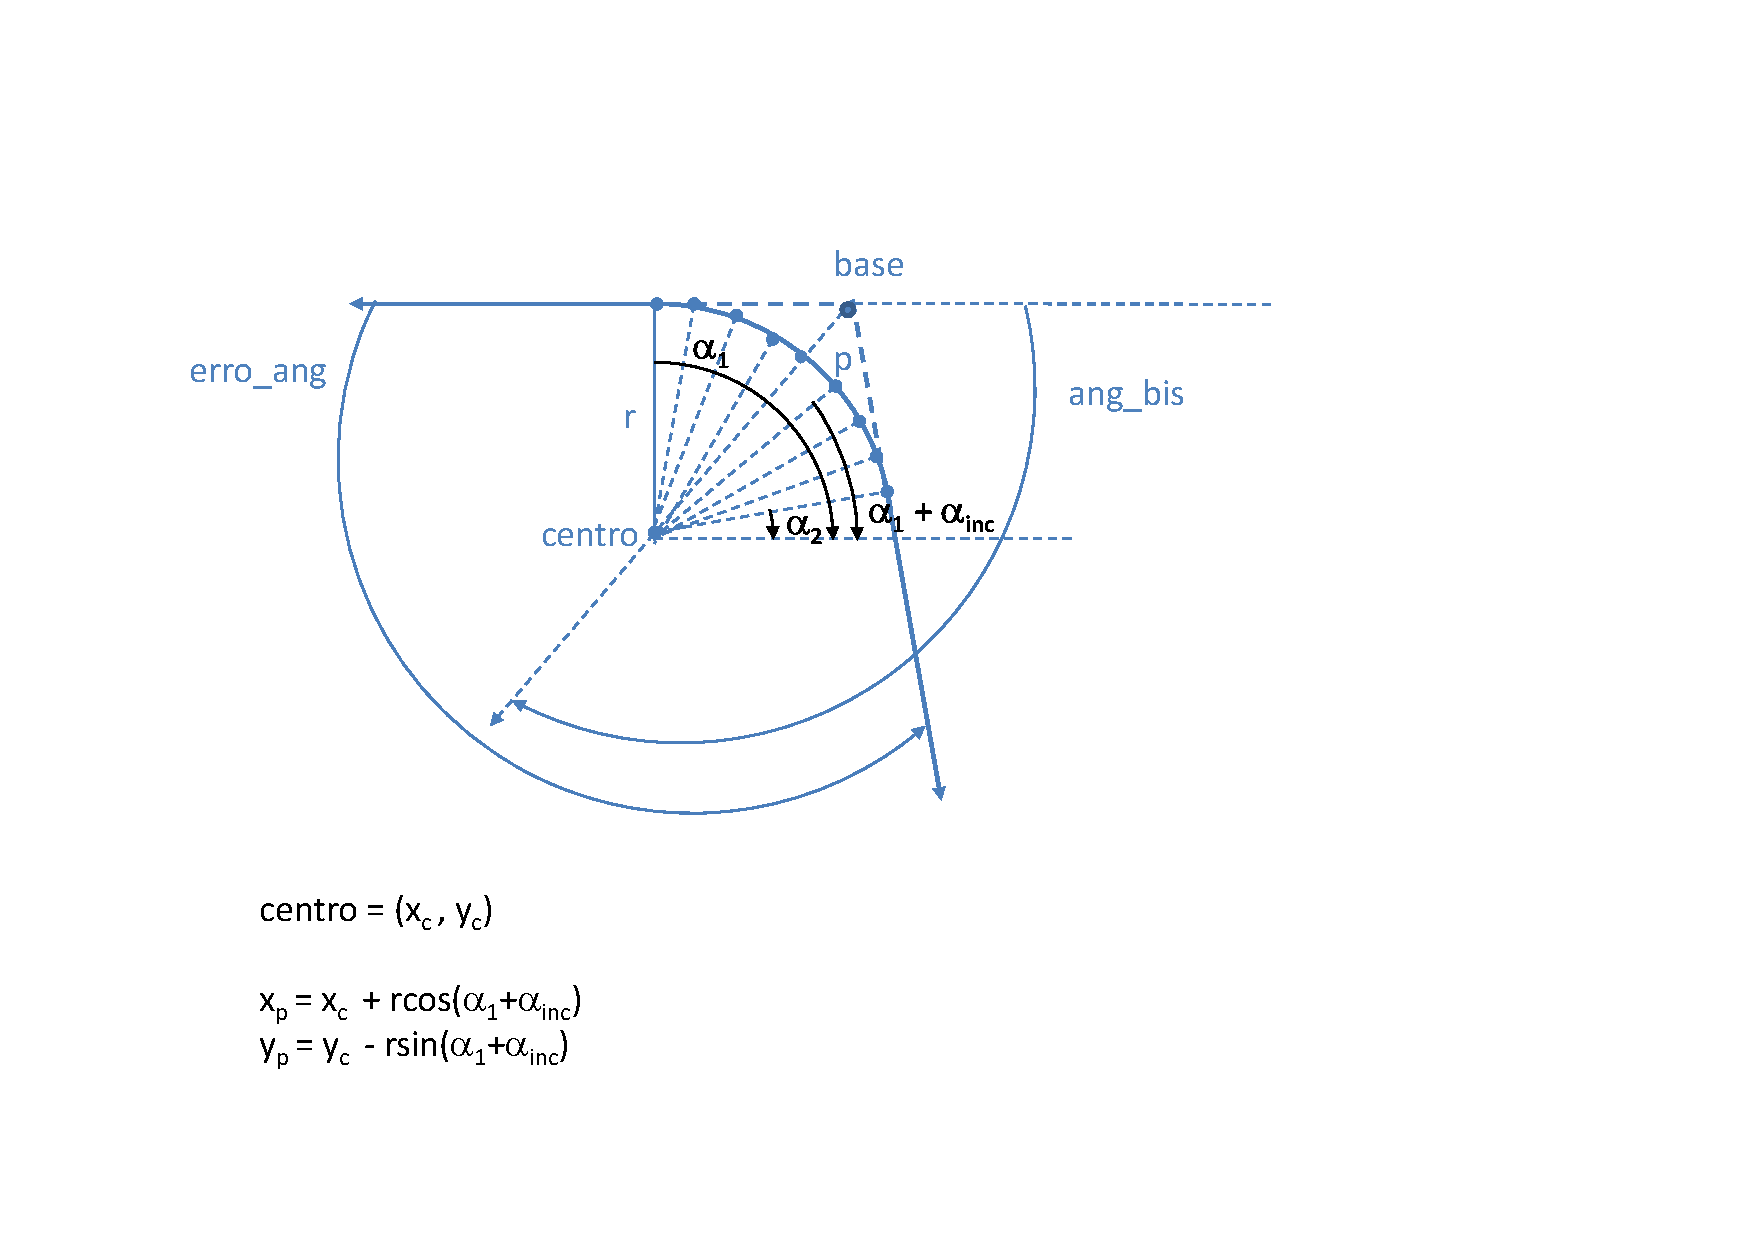
\includegraphics[scale=0.6]{smooth}\\
  \caption{Cálculo de coordenadas de los puntos del arco con 
  $\mbox{erro\_ang} > 0$}\label{fg:smooth}
\end{figure}

En la figura \ref{fg:smooth} se muestra un caso en el que \prog{erro\_ang} es mayor que cero. Para la obtención de los sucesivos puntos el valor de $ang_{inc}$ se va incrementando en 0.1 rad mientras que al sumarse a $\alpha_{1}$ no se sobrepase el valor de $\alpha_{2}$. Estos dos ángulos vienen dados por:

\begin{eqnarray*}
\alpha_{1}  & = & \mbox{AngRango} \left ( alpha\_ref - 
   \left (\frac{\pi}{2} - \frac{\mbox{erro\_ang}}{2} \right ) \right )\\
 \alpha_{2}  & = & \mbox{AngRango} \left ( alpha\_ref + 
   \left (\frac{\pi}{2} - \frac{\mbox{erro\_ang}}{2} \right ) \right )\\
\end{eqnarray*}

Así, para la trayectoria de la figura \ref{fg:smooth} los valores son:
\begin{eqnarray*}
\mbox{erro\_ang}  & = & 100º \\
\mbox{alfa\_ref}     &=  & \mbox{AngRango} (\pi - (-130º))\\
                                  & = &\mbox{AngRango} (310º) \\
                                  & = & -50º\\
alpha_{1}                &= & \mbox{AngRango} (-50º - 90º + 50º)\\ 
                                 & = & \mbox{AngRango} (-90º)\\
                                 & = & -90º\\ 
alpha_{2}                &= & \mbox{AngRango} (-50º + 90º - 50º)\\ 
                                 & = & \mbox{AngRango} (-10º)\\
                                 & = & -10º\\                             
\end{eqnarray*}



Si \prog{erro\_ang} es menor que cero, los ángulos extremos mediante los cuales se calculan las coordenadas de los puntos del arco son:

\begin{eqnarray*}
\alpha_{1}  & = & \mbox{AngRango} \left ( alpha\_ref + 
   \left (\frac{\pi}{2} + \frac{\mbox{erro\_ang}}{2} \right ) \right )\\
 \alpha_{2}  & = & \mbox{AngRango} \left ( alpha\_ref - 
   \left (\frac{\pi}{2} + \frac{\mbox{erro\_ang}}{2} \right ) \right )\\
\end{eqnarray*}

Ahora el ángulo $\alpha_{dec}$, figura \ref{fg:smooth2}, se va decrementando 0.1 rad hasta que su suma con $\alpha_{1}$ se hace menor que $\alpha_{2}$.

\begin{figure}[hbt]
  % Requires \usepackage{graphicx}
  \centering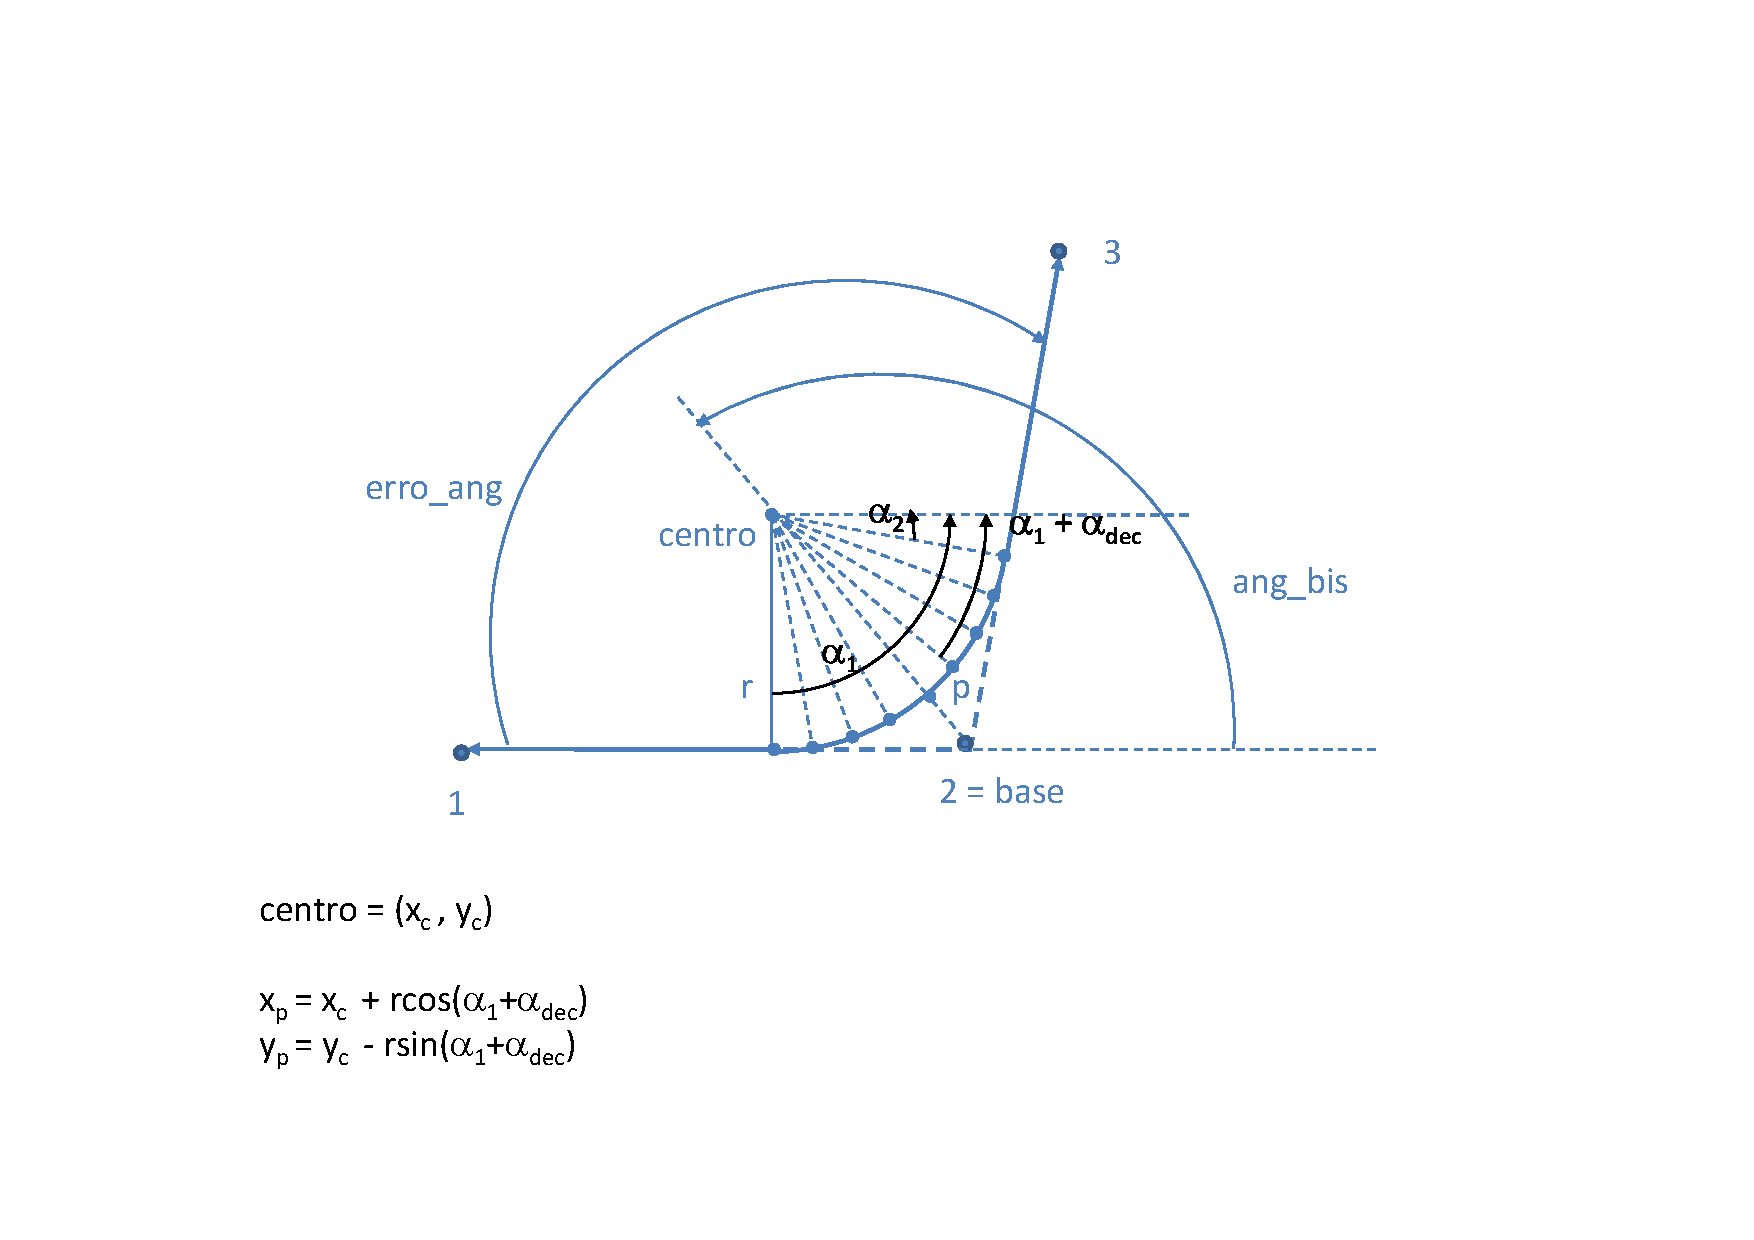
\includegraphics[scale=0.6]{smooth2}\\
  \caption{Cálculo de coordenadas de los puntos del arco con erro\_ang $< 0$}\label{fg:smooth2}
\end{figure}

En el caso concreto representado en la figura \ref{fg:smooth2} los ángulos que se muestran toman los siguientes valores:
\begin{eqnarray*}
\mbox{erro\_ang}  & = & -100º \\
\mbox{alfa\_ref}     &=  & \mbox{AngRango} (\pi - 130º)\\
                                  & = &\mbox{AngRango} (50º) \\
                                  & = & 50º\\
alpha_{1}                &= & \mbox{AngRango} (50º + 90º - 50º)\\ 
                                 & = & \mbox{AngRango} (-90º)\\
                                 & = & -90º\\ 
alpha_{2}                &= & \mbox{AngRango} (50º - 90º + 50º)\\ 
                                 & = & \mbox{AngRango} (-10º)\\
                                 & = & 10º\\                             
\end{eqnarray*}

\clearpage

A continuación se muestra el resultado de aplicar el sistema implementado a diferentes trayectorias. Como puede verse, el color negro representa la trayectoria original y el azul, la trayectoria suavizada. El valor del radio utilizado es 1m.

\begin{figure}[hbt]
  % Requires \usepackage{graphicx}
  \centering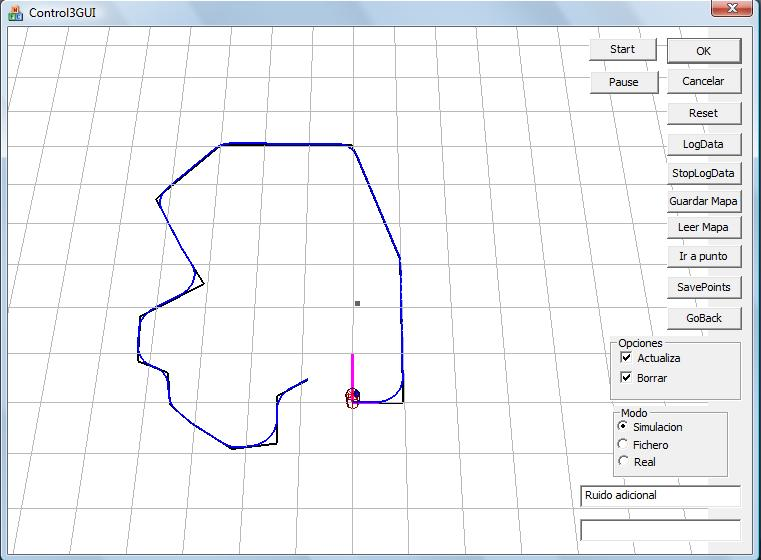
\includegraphics[scale=0.5]{SmoothT}\\
  \vspace{0.2cm}
  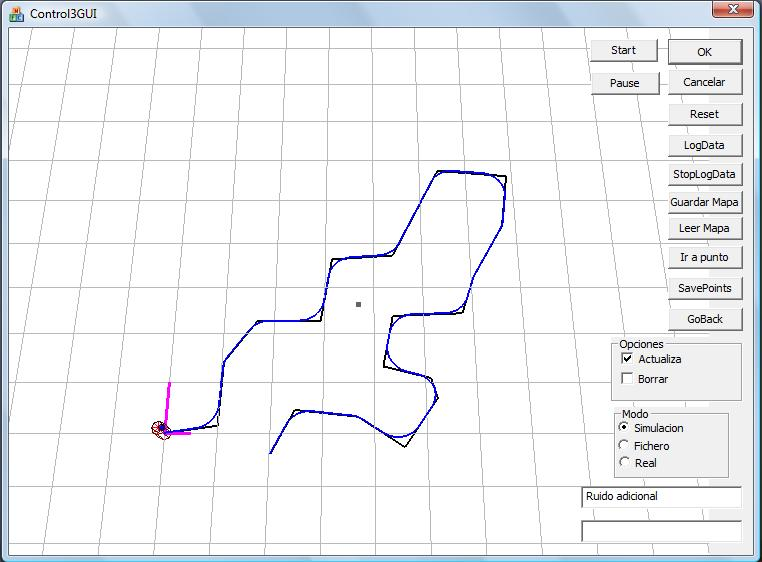
\includegraphics[scale=0.5]{SmoothT2}\label{fg:smoothT}
  \caption{Trayectorias suaves conseguidas}
\end{figure}

\section{Control Reactivo}\label{reactivo}

Una trayectoria planificada y modificada de acuerdo con los apartados anteriores puede requerir nuevos cambios si se detectan obstáculos cercanos a ella. Este aspecto se contempla en el proyecto a través de de un algoritmo que desvía los puntos de la trayectoria cercanos a los objetos. Para cada punto $i$ de la trayectoria nominal se siguen los mismos pasos. En primer lugar, se define un punto $p$ sobre la perpendicular al segmento que une ese punto de la trayectoria con el siguiente de forma que su distancia a dicho punto de la trayectoria sea 1m (ver figura \ref{fg:elastic}). El vector que une el punto de la trayectoria con el punto $p$ se denominará $v_{1}$.

\begin{figure}[hbt]
  % Requires \usepackage{graphicx}
  \centering\includegraphics[scale=0.6]{elastic}\\
  \caption{Definición del punto $p$ y otras magnitudes para el punto de la trayectoria $i = 0$}\label{fg:elastic}
\end{figure}

%%%%%%%%%% pg 82 %%%%%%%%%%%%%%%%%%%%%%%%%%%%%

\pagebreak[4]
Se define un vector $v_{2}$ con origen en el punto de la trayectoria considerado y extremo los sucesivos puntos tomados como obstáculos. La proyección ortogonal de este vector sobre $v_{1}$ define un punto que llamaremos $p_{2}$. La distancia entre éste y el punto de la trayectoria se denota como $d$, que puede adoptar un signo u otro dependiendo de a qué lado de la trayectoria se encuentre el objeto. La distancia entre $p_{2}$ y el obstáculo correspondiente se mide mediante $d_{1}$.

En la deformación de la trayectoria sólo se utilizan los obstáculos que proporcionan un valor de $d_{1}$ suficientemente pequeño, puesto que la influencia de los objetos cercanos a tramos más avanzados de aquella podría llevar a malos resultados.

\begin{figure}[h]
  % Requires \usepackage{graphicx}
  \centering\includegraphics[scale=0.5]{d1}\\
  \caption{Los obstáculos del tramo 1 no deben afectar al 2 ni los del tramo 4 a los tramos 3 y 5.}\label{fg:d1}
\end{figure}

A través de un valor de $d$ corregido al tenerse en cuenta el radio del robot, se guardan para cada punto de la trayectoria las dos distancias mínimas a algún obstáculo a cada uno de los dos lados de la misma. Estas distancias se llamarán min\_int[i] y max\_int[i] respectivamente. Sus valores están inicializados con la máxima desviación que se le permite al robot, para el caso en que no haya ningún obstáculo en alguno de los lados y otras situaciones similares. Si después de recalcular dichos valores se cumple que min\_int $>$ max\_int, el robot no puede evitar los obstáculos sin superar la máxima desviación establecida y se dice que se encuentra en estado de bloqueo.

Haciendo la media entre esos dos valores se obtiene el desplazamiento, error [i], que debe aplicarse sobre el punto para que quede a la misma distancia de cada uno de los límites hallados para ambos lados (figura \ref{fg:elasticTray}).

\begin{figure}[h]
  % Requires \usepackage{graphicx}
  \centering\includegraphics[scale=0.6]{elasticTray}\\
  \caption{Desplazamiento que sufre cada punto de la trayectoria}\label{fg:elasticTray}
\end{figure}

Con los puntos intermedios de la trayectoria lo que se hace es promediar el valor del error en el punto considerado con los valores del mismo en los puntos anterior y siguiente:

\begin{center}
$error2[i] = \frac{error[i-1] + error[i] + error[i+1]}{3}$
\end{center}

\noindent
De este modo se busca deformar la trayectoria más suavemente.

\section{La clase \prog{CMoveControl}}
En esta clase se llevan a cabo las tareas de control de movimiento, planificacón de trayectorias y control reactivo que se han descrito. Las principales funciones que se utilizan para ello son las siguientes:

\subsection{\prog{DefineDest}}

\noindent
\prog{void DefineDest(float x_d, float y_d, float tol)}

\noindent
Esta función sirve para definir el punto hacia el que tiene que dirigirse el robot.

\begin{itemize}
  \item \prog{x_d}: coordenada x del punto de destino.
  \item \prog{y_d}: coordenada y del punto de destino.
  \item \prog{tol}: distancia máxima al punto de destino para que se considere que éste ha sido alcanzado. Generalmente se utiliza una tolerancia de 50mm.
\end{itemize}

\noindent
Se guardan los argumentos en variables miembro, para que sus valores sean utilizados por el control de movimiento, y se establece el estado como \prog{NO_LLEGADO} mediante una macro con este nombre.

\subsection{\prog{Dist2Tray}}

\noindent
\prog{float Dist2Tray()}

\noindent
Esta función se utiliza para hallar la distancia del robot al segmento que une los puntos de la trayectoria entre los que se encuentra e indicar a qué lado del mismo está, de modo que pueda realizarse el control de acercamiento a la trayectoria descrito en \ref{control}.

\noindent
El cálculo de la distancia se lleva a cabo mediante los ángulos mostrados en la figura \ref{fg:dist2tray}, con la fórmula que aparece en ella. El valor que se devuelve es el de $d$.

\subsection{\prog{FindPoint}}

\noindent
\prog{int FindPoint()}

\noindent
Esta función se utiliza para ver cuál es el próximo punto de la trayectoria hacia el que debe ir el robot. Es útil en el caso de que haya pasado demasiado rápidamente por algún punto, para evitar que tenga que retroceder (ver última parte de \ref{control}).

\noindent
Se busca entre los cinco puntos de la trayectoria siguientes al de índice \prog{current_point} dentro del vector \prog{trajectory} aquel que esté más cerca del robot. Se devuelve el valor de su índice.

\subsection{\prog{GetCommand}}

\noindent
\prog{int GetCommand(float* vd, float* vs)}

\noindent
La función de este método consiste en calcular las velocidades de avance y giro con los que se va a mover el robot en cada momento. El paso de parámetros se realiza por referencia.

\begin{itemize}
  \item \prog{vd}: puntero a la velocidad de avance.
  \item \prog{vs}: puntero a la velocidad de giro.
\end{itemize}

\noindent
En primer lugar se mira si es necesario corregir el punto de destino con una llamada a la función \prog{FindPoint()} y si es así se hacen los correspondientes cambios. A continuación se determina el estado, viendo si la distancia entre la posición del robot y el punto de destino es menor que la tolerancia.

En la figura se muestra el diagrama de flujo simplificado de los pasos que se realizan a partir de este punto.

\begin{figure}[h]
  % Requires \usepackage{graphicx}
  \centering\includegraphics[scale=0.6]{flujo1}\\
  \caption{Diagrama de flujo simplificado de parte del proceso efectuado en \prog{GetCommand}}\label{fg:flujo1}
\end{figure}
Si el estado es \prog{NO_LLEGADO}, se determinan las velocidades mediante el procedimiento indicado en \ref{control} a partir de la posición del robot (disponible en toda la clase mediante las variables miembro \prog{x} e \prog{y}) y del punto guardado como destino.
Si el estado es \prog{LLEGADO} se da valor nulo a ambas velocidades y se incrementa una variable llamada \prog{current_point} que mide de este modo el índice del último punto de la trayectoria al que se ha llegado. Si efectivamente hay una trayectoria definida, se llama a la función \prog{DefineDest} para guardar como destino el siguiente punto de la misma (\prog{current_point + 1}). Los puntos de la trayectoria han de estar almacenados en un vector de la STL, vector \prog{trajectory}, miembro de la clase y definido para contener objetos CPoint2D.
\noindent
El valor de retorno es el estado.

\subsection{\prog{DefineTrajectory}}

\noindent
\prog{void DefineTrajectory(void)}

\noindent
Esta función se emplea para indicar que hay una trayectoria definida e inicializar el punto por el que debe empezarse a recorrerla (\prog{current_point = 0}).

\subsection{\prog{SmoothTrajectory}}

\noindent
\prog{std::vector<Point2D> SmoothTrajectory(float r)}

\noindent
Esta función se utiliza para suavizar la trayectoria.
\begin{itemize}
  \item \prog{r}: radio del arco con el que se suavizan los ángulos de la trayectoria.
\end{itemize}

\noindent
Los puntos de la trayectoria a suavizar se hallan guardados en un vector dinámico de nombre \prog{tray_prev} e inicialmente se copian en otro vector dínámico variable local de la función (vector \prog{smooth_tray}) para realizar en éste las modificaciones oportunas y no perder los puntos de la trayectoria original (de cara a la representación gráfica, principalmente).
Esta función es la implementación del algoritmo descrito en \ref{tray}. Se devuelve el vector \prog{smooth_tray}, que contiene los puntos de la trayectoria suave obtenida.

\subsection{\prog{ComputeElasticTray}}

\noindent
\prog{std::vector<Point2D> ComputeElasticTray()}

\noindent
Esta función sirve para deformar la trayectoria de forma que se aleje de los obstáculos (puntos 2D guardados en el vector de la STL \prog{v_puntos}, variable miembro de la clase).

\noindent
Los puntos de la trayectoria que se deforma son los almacenados en el vector \prog{nom_tray} de la STL, que se copian en una variable local de nombre \prog{ret_tray}. Con estos puntos se siguen los pasos indicados en el algoritmo de \ref{reactivo}. En caso de que al calcularse alguno de los nuevos puntos se produzca bloqueo (\prog{min_int[i] > max_int[i]}), se devuelve la trayectoria \prog{ret_tray} con los puntos hallados hasta ese momento. Si no se da situación de bloqueo, el vector \prog{ret_tray} se devuelve al final de la función y tendrá tantos puntos como la trayectoria inicial. El resultado de esta llamada será asignado al vector \prog{trajectory} para que pueda aplicarse el control de movimiento.

%\subsection{\prog{FindPoint}}
%
%\noindent
%\prog{int FindPoint()}
%
%\noindent
%Esta función se utiliza para ver cuál es el próximo punto de la trayectoria hacia el que debe ir el robot. Es útil en el caso de que haya pasado demasiado rápidamente por algún punto, para evitar que tenga que retroceder (ver última parte de \ref{control}).
%
%\noindent
%Se busca entre los cinco puntos de la trayectoria siguientes al de índice \prog{current_point} dentro del vector \prog{trajectory} aquel que esté más cerca del robot. Se devuelve el valor de su índice.

\subsection{\prog{DivideTrajectory}}

\noindent
\prog{int DivideTrajectory()}

\noindent
Esta función permite obtener una trayectoria igual a la inicial (\prog{nom_tray}) pero con el requisito de que cada uno de sus puntos no diste más de 0.1m del siguiente.


\noindent
Se utiliza un vector de la STL, variable local de la función, en el que se guarda cada punto de la trayectoria seguido de tantos otros puntos como sea necesario para que el segmento que va de aquél al próximo punto de \prog{nom_tray} cumpla la condición dada. El número de puntos intermedios que se añaden será $n = \frac{dist}{0.1} - 1$, siendo $dist$ la longitud del segmento inicial. Finalmente se iguala el vector \prog{nom_tray} al vector con los nuevos puntos.

\begin{figure}[h]
  % Requires \usepackage{graphicx}
  \centering\includegraphics[scale=0.6]{divide}\\
  \caption{Puntos de un segmento de la trayectoria original y del resultado de la llamada a \prog{DivideTrajectory()}}\label{fg:divide}
\end{figure}

\vspace{0.2cm}

\noindent
La utilidad de esta función reside en la necesidad de tener los puntos de la trayectoria suficientemente juntos para que el control reactivo que se implementa a través de \prog{ComputeElasticTray()} sea efectivo. Si no fuera así, el filtro que se realiza mediante $d_{1}$ no permitiría esquivar muchos de los obstáculos.

%\subsection{\prog{Dist2Tray}}
%
%\noindent
%\prog{float Dist2Tray()}
%
%\noindent
%Esta función se utiliza para hallar la distancia del robot al segmento que une los puntos de la trayectoria entre los que se encuentra e indicar a qué lado del mismo está, de modo que pueda realizarse el control de acercamiento a la trayectoria descrito en \ref{control}.
%
%\noindent
%El cálculo de la distancia se lleva a cabo mediante los ángulos mostrados en la figura \ref{fg:dist2tray}, con la fórmula que aparece en ella. El valor que se devuelve es el de $d$.


\section{Pruebas y resultados}
Todas las funcionalidades de control de movimiento, planificación de trayectorias y control reactivo del proyecto han sido probadas inicialmente mediante simulación gráfica. Esto permite la depuración y mejora del comportamiento del programa de una forma más cómoda. Las pruebas con robots reales requieren más espacio y pueden conllevar mayores riesgos si no se han llevado a cabo previamente en simulación. Además, es preciso cargar baterías, llevar el ejecutable al ordenador portátil que se utiliza, realizar la conexión \emph{telnet} e introducir las contraseñas correspondientes\ldots por lo que resultan bastante más lentas. El control de movimiento, sin embargo, sí que fue probado en modo real en fases anteriores del proyecto ya que la respuesta del robot ante las velocidades aplicadas puede ser algo diferente en uno y otro caso y resultaba conveniente ajustar bien los parámetros para no seguir trabajando con un regulador inadecuado.

\subsection{Pruebas en modo \emph{simulación}}

\subsubsection{Control de movimiento y planificación de trayectorias}

\noindent
\textbf{\textbf{1.} Seguimiento de una trayectoria planificada a priori}

En este caso, lo que se ha hecho es definir los puntos de la trayectoria inicial mediante doble click con el botón derecho del ratón sobre la interfaz gráfica. Según se van añadiendo puntos se va suavizando la trayectoria. Cuando se ha completado la definición de la trayectoria deseada se indica que el robot debe seguirla y éste comienza a moverse sobre la misma. En la figura puede verse en color azul la trayectoria resultante tras la planificación, en verde la trayectoria seguida de acuerdo con las medidas de la odometría y en rojo la trayectoria seguida según la localización. Como las medidas del láser en modo simulación se hallan a 8000m del robot (ver método \prog{Simulate}, de \ref{CPosData}), no se realiza asociación de datos ni se corrige la posición, de modo que las trayectorias dibujadas en verde y rojo serán necesariamente iguales. La única diferencia reside en el hecho de que se han representado a diferentes alturas.


\textbf{Resultados:}
\begin{figure}[h]
  % Requires \usepackage{graphicx}
  \centering\includegraphics[scale=0.4]{mov1}\\
  \caption{Primer experimento de planificación de trayectorias y control de movimiento}\label{fg:mov1}
\end{figure}

Como puede verse, la trayectoria seguida por el robot es prácticamente idéntica a la planificada, lo que muestra el buen diseño del controlador.

\noindent
\textbf{\textbf{2.} Seguimiento de una trayectoria planificada a priori con el robot Pioneer P3AT}

Esta es una de las pruebas que se realizó con el control elaborado para el robot Pioneer P3AT de MobileRobots/Activmedia. En ella se utiliza MobileSim, un software de simulación proporcionado por los fabricantes para la experimentación con Aria. MobileSim está construido sobre el simulador Stage (creado por Richard Vaughan, Andrew Howard y otros como parte del proyecto Player/Stage), con algunas modificaciones por parte de MobileRobots. Utilizando la clase \prog{SimpleConnector} de la biblioteca Aria, la conexión se inicia por defecto con el simulador.


\textbf{Resultados:}
\begin{figure}[h]
  % Requires \usepackage{graphicx}
  \centering\includegraphics[scale=0.4]{mov2}\\
  \caption{Segundo experimento de planificación de trayectorias y control de movimiento}\label{fg:mov2}
\end{figure}

La trayectoria inicial definida en este caso es la formada por los puntos marcados en negro. Puede observarse que el control proporciona de nuevo un buen resultado.

\noindent
\textbf{\textbf{3.} Seguimiento de una trayectoria planificada dinámicamente}

En esta prueba se generan nuevos puntos de la trayectoria a medida que el robot se acerca a su próximo destino. En algunos casos, al llegar el robot a un punto y posteriormente añadir otro punto después de aquél, el algoritmo que suaviza la trayectoria hace que ésta deje de pasar por el punto en el que se encontraba el robot. Si se produce esta circunstancia, entra en acción el controlador para evitar desvíos sobre la trayectoria planificada. El buen funcionamiento del mismo puede verse con claridad en las figuras \ref{fg:mov3} y \ref{fg:mov4}:



\textbf{Resultados:}
\begin{figure}[h]
  % Requires \usepackage{graphicx}
  \centering\includegraphics[scale=0.4]{mov3}\\
  \vspace{2cm}\includegraphics[scale=0.4]{mov_3}
  \caption{Tercer experimento de planificación de trayectorias y control de movimiento}\label{fg:mov3}
\end{figure}


En la segunda figura, por ejemplo, el robot llega al punto B procedente del A y, seguidamente, se añade a la trayectoria el punto C. El algoritmo para suavizar trayectorias redondea entonces la trayectoria que habría de estar formada por A, B y C, pero el robot ya se encuentra en B. El regulador inicial conduciría al robot directamente hacia C pero las mejoras introducidas hacen que el robot se aproxime primero a la trayectoria planificada.

\noindent
\textbf{\textbf{4.} Seguimiento del camino de vuelta después de que el robot ejecute una trayectoria.}

En este caso, se define una trayectoria mediante el ratón o moviendo al robot por teleoperación con el teclado (sección \ref{opciones}). Cuando finaliza el seguimiento de la misma, el robot es capaz de regresar de forma autónoma al punto de partida si así se le indica. En la primera figura que se muestra, la trayectoria inicial está definida mediante el ratón mientras que en la segunda se utiliza el modo teleoperado. La trayectoria dibujada en color verde es la correspondiente a la odometría durante la ida y la que aparece en rosa es la odometría del camino de vuelta.

\textbf{Resultados:}
\begin{figure}[h]
  % Requires \usepackage{graphicx}
  \centering\includegraphics[scale=0.4]{vuelta}\\
  \hspace{0.5cm}\includegraphics[scale=0.4]{vuelta2}
  \caption{Cuarto experimento de planificación de trayectorias y control de movimiento}\label{fg:mov4}
\end{figure}


\subsubsection{Control reactivo}

\noindent
\textbf{\textbf{1.} Obtención de trayectorias deformadas ante la presencia de obstáculos cercanos a una trayectoria definida}
En esta prueba se define primeramente una trayectoria y a continuación se crean obstáculos más o menos cercanos a la misma mediante doble click con el botón izquierdo del ratón sobre el punto en el que debe situarse cada uno de ellos. En el momento en que se añade un obstáculo, la trayectoria se deforma mediante el algoritmo previamente explicado. En este caso no se han incorporado obstáculos nuevos durante el movimiento del robot sobre la trayectoria, por lo que no se trata de una aplicación de control reactivo sino sólo de una prueba del algoritmo de deformación.

\textbf{Resultados:}
\begin{figure}[h]
  % Requires \usepackage{graphicx}
  \centering\includegraphics[scale=0.4]{obs2}\\
  \hspace{0.5cm}\includegraphics[scale=0.4]{obs3}
  \caption{Experimento previo para el control reactivo}\label{fg:react1}
\end{figure}


Como puede verse, los obstáculos se han representado en color cyan. La trayectoria se deforma de un modo suave en los puntos cercanos a ellos sin superar la máxima desviación permitida, establecida en 0.15m. Los obstáculos suficientemente alejados de la trayectoria no suponen ninguna modificación en la misma. En la segunda figura hay un obstáculo que afecta a dos tramos diferentes de la trayectoria y ambas deformaciones se realizan correctamente. Con este valor de la máxima desviación permitida no pueden esquivarse obstáculos que se encuentren sobre la trayectoria a seguir. En este caso, para el robot Urbano, entrarían en acción los mecanismos de control reactivo de bajo nivel (comandos de parada y giro). Si se utiliza en su lugar un valor de 0.6m, las deformaciones son mayores y pueden evitarse los obstáculos que supondrían un choque directo (figura \ref{react2}). El problema que conlleva esta opción es que en el caso de entornos densos (como son la mayoría de los entornos de interiores), las deformaciones son excesivas hacia uno y otro lado y se pierde suavidad en la trayectoria.
\begin{figure}[h]
  % Requires \usepackage{graphicx}
  \centering\includegraphics[scale=0.4]{obs4}\\
  \caption{Aumento de la máxima desviación permitida}\label{fg:react2}
\end{figure}


\noindent
\textbf{\textbf{2.} Trayectoria seguida por el robot ante la aparición de un obstáculo durante su movimiento sobre una trayectoria}

En este caso se ha llevado el robot a un punto por medio de una trayectoria definida sobre la interfaz gráfica y se le ha indicado que regrese a su posición inicial. Durante el camino de vuelta, se ha creado un obstáculo en la trayectoria teórica que debería seguir el robot para ver su respuesta simulada en tiempo real.

\textbf{Resultados:}
En la figura \ref{fg:react3} se ha plasmado en color verde la trayectoria seguida por el robot durante la ida (trayectoria teórica de vuelta) y en colores azul y magenta la trayectoria real efectuada ante la presencia del obstáculo.
\begin{figure}[h]
  % Requires \usepackage{graphicx}
  \centering\includegraphics[scale=0.4]{react2}\\
  \caption{Primer experimento de control reactivo}\label{fg:react3}
\end{figure}


\subsection{Pruebas en modo \emph{real}}
Cuando se utiliza el sistema con el robot real las llamadas a \prog{GetCommand} se realizan cada 300ms aproximadamente. Como se verá en los siguientes resultados, el seguimiento de la trayectoria es algo menos preciso que en las pruebas realizadas en simulación.

\subsubsection{Control de movimiento y planificación de trayectorias}

\noindent
\textbf{\textbf{1.} Seguimiento de una trayectoria planificada a priori}
En estas pruebas lo que se ha hecho es definir una trayectoria con el ratón, al igual que en el modo simulación, y ver cómo el robot se va dirigiendo hacia los correspondientes puntos de la misma. La longitud de las trayectorias efectuadas está limitada por el entorno de experimentación, una zona del laboratorio no muy amplia y con objetos cercanos que disminuyen el área explorable.

\textbf{Resultados:}
En la figura \ref{fg:real1} se muestra en color azul la trayectoria nominal seleccionada y en colores verde y rojo la seguida por el robot.
\begin{figure}[h]
  % Requires \usepackage{graphicx}
  \centering\includegraphics[scale=0.4]{real}\\
  \hspace{0.5cm}\includegraphics[scale=0.4]{real1}
  \caption{Primer experimento de movimiento con robot real}\label{fg:real}
\end{figure}

En el segundo caso se aprecia que el mantenimiento de la dirección de la trayectoria prevalece frente a la acción de acercar el robot a la misma, pero esto evita que la trayectoria resultante sea más ondulada.

\noindent
\textbf{\textbf{2.} Seguimiento del camino de vuelta después de que el robot ejecute una trayectoria.}
La forma de proceder en este caso es la misma que en el modo de simulación.
\textbf{Resultados:}
En la figura \ref{fg:real2} se muestra en color verde la trayectoria durante la ida y en color rosa la correspondiente al camino de vuelta.
\begin{figure}[h]
  % Requires \usepackage{graphicx}
  \centering\includegraphics[scale=0.4]{real2}\\
  \caption{Segundo experimento de movimiento con robot real}\label{fg:real2}
\end{figure}

Como puede observarse, en este caso aparecen mayores desviaciones respecto a la trayectoria definida. La desviación producida al dar la vuelta el robot hace que éste tarde un poco en coger la dirección correcta, pero las acciones de control sobre err\_ang2 y err\_ang3 permiten que los cambios no sean demasiado bruscos. Si la trayectoria fuera más larga podría verse que la estabilización es bastante rápida.

% -*- coding: utf-8 -*-

\chapter{Integración}\label{ch:integracion}

El funcionamiento del sistema requiere la integración de sus distintos componentes. El robot debe combinar su capacidad para localizarse correctamente en el entorno con el seguimiento de una trayectoria adecuada, resultante de la planificación y el control reactivo. La localización resulta imprescindible para el buen funcionamiento del control y, particularmente, para situaciones en que el robot quede alejado de la trayectoria definida (como en la figura \ref{fg:reg}%
%\footnote{Página \pageref{fg:reg}}%
).

La interacción entre el módulo de localización y el de control de movimiento se lleva a cabo mediante la clase \prog{CRobot}, como puede apreciarse en el diagrama \ref{fg:uml}.%
%\footnote{Página \pageref{fg:uml}}
Desde las clases \prog{CRobotGLWnd} y \prog{CControl3GUIDlg} se realiza la transferencia de información desde la interfaz gráfica al resto del programa. En esta última se tiene el objeto \prog{gl_wnd}, de la clase \prog{CRobotGLWnd}, el objeto \prog{robot}, de la clase \prog{CRobot} y el objeto \prog{control}, de la clase \prog{CMoveControl}. Desde \prog{robot} se tiene un puntero al objeto \prog{control}. Desde \prog{gl_wnd} se tienen punteros a  \prog{robot} y a \prog{control} (para simplificar las llamadas a sus métodos y no tener que utilizarlos a través del puntero al objeto \prog{robot}).

\section{La clase \texttt{CRobot}}
El papel de esta clase consiste en integrar:
\begin{itemize}
  \item la obtención de los datos de odometría y del láser
  \item la estimación o/y corrección de la posición mediante el filtro de Kalman y la actualización del mapa
  \item el paso de la posición corregida y del mapa de obstáculos al módulo de control de movimiento
\end{itemize}
Para ello se dispone de algunas variables miembro importantes:
\begin{itemize}
  \item \prog{robotdata}, de la clase \prog{CRobotDataReal}
  \item \prog {proc_laser_data}, de la clase \prog{CProc_Laser_Data}
  \item \prog{loc}, de la clase \prog{CKalman_Loc}
  \item \prog{control}, puntero a un objeto de la clase \prog{CMoveControl} (que habrá de apuntar al objeto \prog{control} miembro del diálogo \prog{CControl3GUIDlg}).
\end{itemize}
%\noindent
También posee una variable puntero a un objeto de tipo \prog{CPioneer}, para las pruebas de control que se han hecho con el robot P3AT.

%Las funciones que forman parte de la clase son las siguientes:

%\subsection{SetPioneer}
%
%\noindent
%\prog{void SetPioneer(CPioneer* pioner)}
%
%\noindent
%Esta función se emplea para hacer que el puntero miembro de \prog{CRobot} apunte a un objeto \prog{CPioneer} determinado que se le pasa como parámetro.
%
%\begin{itemize}
%  \item \prog{pioner}: puntero al objeto de la clase \prog{CPioneer} al que se quiere apuntar desde un objeto \prog{CRobot}.
%\end{itemize}
%
%\subsection{SetControl}
%
%\noindent
%\prog{void SetControl(CMoveControl* cont)}
%
%\noindent
%Esta función se utiliza para hacer que el puntero miembro de \prog{CRobot} apunte a un objeto \prog{CMoveControl} determinado que se le pasa como parámetro.
%
%\begin{itemize}
%  \item \prog{cont}: puntero al objeto de la clase \prog{CMoveControl} al que se quiere apuntar desde un objeto \prog{CRobot}.
%\end{itemize}
%
%\subsection{shutdown}
%
%\noindent
%\prog{void shutdown()}
%
%\noindent
%Esta función sirve para desconectar el robot Pioneer en caso de que se esté utilizando.

\subsection{\texttt{ProcessData}}

\noindent
\prog{int ProcessData()}

\noindent
Es la función principal de la clase. Sirve para integrar los componentes que se han indicado anteriormente.

\noindent
En primer lugar se actualizan los datos odométricos y del láser mediante \prog{robotdata.UpdateData()}.

Si se han obtenido datos de la odometría (valor de retorno \prog{ODOM_DATA} o \prog{DATA_ODOM_LASER}) se calcula el incremento que ha de utilizarse para la etapa de predicción del algoritmo de localización a partir de la transformación inversa de la posición odométrica previa y su composición con la posición odométrica recién obtenida. La nueva posición se guarda como posición antigua para la siguiente llamada a la función. En caso de que se haya añadido un ruido adicional (a través del cuadro de diálogo), se inyecta éste en el incremento de odometría mediante composición con aquél. La posición odométrica con el ruido extra se guarda en un vector de la STL para su representación gráfica. Por último se calcula la predicción de la posición odométrica mediante \prog{loc.KalmanPos} con los argumentos correspondientes al incremento de odometría calculado.

Si se han obtenido datos del láser (\prog{robotdata.UpdateData()} ha devuelto \prog{LASER_DATA} o \prog{DATA_ODOM_LASER}) lo primero que se hace es procesar la información del mismo que estará disponible en la variable de la clase \prog{CRawLaserData} perteneciente a \prog{robotdata} para que en \prog{proc_laser_data} se tenga el vector \prog{v} con los puntos correspondientes a las medidas del láser (llamada a \prog{proc_laser_data}.\prog{DefineData}(\prog{robotdata.laser_data}).
Seguidamente se realizan las operaciones necesarias para calcular los puntos del polígono correspondiente a esa serie de medidas del láser mediante el objeto \prog{proc_laser_data}. Se obtienen también los ángulos $\alpha$ de la figura \ref{fg:poligono} y se pasan éstos y la información del polígono a variables miembro del objeto \prog{loc}. Se calcula la corrección de la posición estimada por medio de \prog{loc.KalmanUpdate}, pasándole como argumento el vector \prog{v} de la variable \prog{proc_laser_data}.

La posición resultante de esta actualización se guarda en un vector de la STL para representar en la interfaz gráfica la trayectoria corregida mediante el algoritmo de localización y poder compararla con la trayectoria basada únicamente en los datos de la odometría.

Esta nueva posición es la que ha de utilizar el control de movimiento. Como las variables \prog{x} y \prog{y} de la clase \prog{CMoveControl} son públicas, basta con asignarles el valor correspondiente a la posición corregida con el filtro de Kalman.

Lo último que se hace es pasarle a la variable \prog{control} el vector con aquellos puntos del mapa (actualizado en la llamada a \prog{ KalmanUpdate}) suficientemente cercanos al robot como vector que contiene los obstáculos a evitar por el control reactivo y efectuar la deformación de la trayectoria mediante \prog{control.ComputeElasticTray()}.

El valor de retorno es 1 si se han actualizado datos de odometría o del láser y 0 en caso contrario.

Esta función va a ejecutarse a modo de bucle, dentro de un \emph{timer} que se define en la clase \prog{CControl3GUIDlg}.

\section{La clase \texttt{CControl3GUIDlg}}
Esta clase hereda de la clase pública \prog{CDialog}, perteneciente a las MFC. En ella comienza el hilo principal de ejecución del programa. Desde esta clase se crea el cuadro de diálogo, al que han de añadirse los diferentes botones para realizar el paso de información del usuario a los distintos componentes del sistema. En ella se tiene la variable \prog{gl_wnd} para crear la ventana gráfica y asociarla a él. Como se ha mencionado, proporciona el modo de controlar el ciclo de tareas que ha de realizar el robot mediante un temporizador o \emph{timer} que permite la repetición de una serie de acciones periódicamente. La variable \prog{robot}, de acuerdo con lo visto, es necesaria para obtener la posición corregida y el mapa y hacer posible su utilización desde el control de movimiento en cada momento. La variable \prog{control} se emplea para facilitar el acceso a aquél. %Las principales funciones editadas en esta clase son:

\section{Interfaz de usuario}
Aunque ya se ha mostrado en otras figuras, a continuación se presenta el aspecto de la interfaz de usuario desarrollada (figura \ref{fg:interfaz}. En esta imagen se ve tal y como aparece al iniciarse la ejecución del programa (salvo los colores de fondo y cuadrícula, que por defecto son negro y magenta pero pueden cambiarse pulsando en el teclado la letra 'F'). Seguidamente se describirán sus propiedades y la utilidad de sus botones.

\begin{figure}[h]
  % Requires \usepackage{graphicx}
  \centering\includegraphics[scale=0.4]{interfazNueva}\\
  \caption{Interfaz de usuario}\label{fg:interfaz}
\end{figure}


\subsection{Funcionalidad de los botones del diálogo}

\subsubsection{OK y Cancelar}

%\noindent
Siempre que se pulse alguno de estos botones se cierra la interfaz de usuario y finaliza la ejecución del programa.

\subsubsection{Reset}
%\noindent
Se emplea para anular la definición de una trayectoria y de una serie de obstáculos realizados mediante el ratón.

\subsubsection{Guardar Mapa}

%\noindent
Se utiliza para guardar los puntos de un mapa en un fichero. Ha de ser pulsado tras finalizar el recorrido del robot por el entorno que se desee representar. Al ser marcado se abre el típico cuadro de Windows \emph{Guardar Como} para seleccionar el directorio y el nombre del fichero. De esta forma, no tienen que realizarse nuevos mapas cada vez sino que pueden ser leídos mediante \emph{Leer mapa}:

\subsubsection{LeerMapa}

%\noindent
Muestra un cuadro de Windows tipo \emph{Abrir} para establecer como mapa los puntos leídos de un fichero creado mediante \emph{Guardar Mapa}.

\subsubsection{Ir a punto}

%\noindent
Se emplea para que el robot siga una trayectoria definida sobre la interfaz gráfica mediante el ratón.

\subsubsection{Guardar Tray}

\noindent
Permite guardar la trayectoria que sigue el robot, para que luego pueda regresar al punto de partida. Ha de pulsarse en el momento en que se desee que empiece a guardarse el camino, normalmente antes de que comience el movimiento del robot.

\subsubsection{Volver}

%\noindent
Cuando se pulsa este botón el robot emprende el camino de regreso por la misma trayectoria seguida hasta el momento.

\subsubsection{Opciones}
Dentro de este grupo de botones de tipo \emph{check-box} se ofrecen algunas alternativas de funcionamiento del sistema:
\begin{itemize}
  \item Actualiza: permite añadir o no puntos al mapa en función de las medidas del láser. Si no se ha leído ningún mapa mediante \emph{Leer Mapa} y no se marca esta opción, el mapa permanecerá vacío y no podrá efectuarse la localización. Puede variarse la condición elegida a lo largo del funcionamiento del sistema.
  \item Borrar: sirve para establecer si se han de borrar los puntos dinámicos mediante el algoritmo del polígono envolvente o no. En caso afirmativo se dibuja sobre la pantalla el polígono correspondiente en cada momento y los puntos que han sido borrados aparecen en color cyan.
\end{itemize}

\subsubsection{Modo}
Este grupo de botones \emph{radio-box} se emplea para seleccionar el tipo de conexión que se desea.
\begin{itemize}
  \item Simulación: establece el funcionamiento del sistema en modo simulación
  \item Fichero: establece el funcionamiento del sistema en modo fichero
  \item Real: establece el funcionamiento del sistema en modo real
\end{itemize}

\subsubsection{LogData}
Permite guardar en un fichero los datos de odometría y del láser mediante la llamada al método \prog{StartLogData} de la clase \prog{CRobotData}.

\subsubsection{StopLogData}
Se utiliza para cerrar el fichero anterior y de este modo dejar de registrar los datos. Básicamente realiza una llamada a \prog{StopLogData} de la clase \prog{CRobotData}.

%\vspace{0.2cm}
%\noindent
\paragraph{Nota:} 
Lógicamente, los dos botones anteriores no se encuentran activados si el modo de funcionamiento es tipo fichero.

\subsubsection{Desviación típica de odometría}
En esta \emph{edit box} puede introducirse el valor de la desviación típica en los datos de la odometría que se ha de utilizar en el filtro de Kalman. Si en ella no se escribe ningún valor, se emplea una desviación típica de 0.1.

\subsubsection{Ruido adicional}
El valor que se introduzca en esta \emph{edit box} será inyectado como ruido adicional a la odometría. Permite evaluar el funcionamiento del algoritmo de localización con distintas calidades de los datos odométricos. Si no se escribe nada en el cuadro, el valor por defecto es 0.

\subsubsection{Mensaje}
En esta \emph{edit box} se muestra información sobre la última acción que se le ha pedido que realice al robot (\emph{Guardando trayectoria}, \emph{Siguiendo trayectoria})...

\subsubsection{Start}
Con este botón se inicia un temporizador para que se ejecute el ciclo de tareas del robot cada cierto tiempo (periodo de 10ms en los modos simulación y fichero y de 150ms en modo real). Conviene utilizarlo una vez se han seleccionado los parámetros de funcionamiento.

\subsubsection{Pause}
Este botón mata el temporizador y con ello dejan de realizarse las actualizaciones del ciclo, por lo que el sistema se mantiene estático hasta que vuelva a lanzarse el ciclo de tareas pulsando de nuevo el botón \emph{Start}.

\subsubsection{Radio}
El valor que se introduzca en esta \emph{edit box} se utilizará como radio de curvatura para suavizar la trayectoria. Si no se escribe nada en ella el valor por defecto es 1m.

\subsubsection{Orientación final}
Esta \emph{edit box} se utiliza si se desea concretar una orientación del robot en el punto final de la trayectoria. Si se ha pulsado la opción de \emph{Volver} la orientación final será por defecto la que tenía el robot en el momento en que se comenzó a guardar la trayectoria. En caso contrario el robot mantendrá la orientación con la que llegue al destino.

\subsubsection{Robot}
Este grupo de botones se utiliza para escoger el tipo de robot que se va a emplear.
\begin{itemize}
  \item Urbano: opciones correspondientes al robot Urbano (B21r de iRobot).
  \item Pioneer: opciones correspondientes al robot Pioneer (P3AT de ActivMedia Robotics).
\end{itemize}

Las principales diferencias entre seleccionar uno u otro robot se hallan en el modo en que se realiza la conexión, en la forma en que se envían los comandos de velocidad y se recibe la información de la odometría y del láser y en los parámetros del control de movimiento. La separación de ambos casos se realiza, por lo tanto, en las clases \prog{CControl3GUIDlg} (conexión en el botón \emph{Start} y envío de comandos en el \emph{timer}), \prog{CRobot} (obtención de las medidas del sistema odométrico y de las observaciones proporcionadas por el láser) y \prog{CMoveControl} (regulador para seguir la trayectoria).

\subsection{Selección de opciones mediante ratón o teclado} \label{opciones}
Por medio del ratón pueden realizarse los siguientes cambios relativos a la visualización:
\begin{itemize}
  \item Acercamiento y alejamiento del punto de vista mediante giro de la rueda del ratón en uno u otro sentido. El mismo resultado se obtiene moviendo el ratón con el botón derecho pulsado.
  \item Variación del punto de vista manteniendo apretado el botón izquierdo del ratón mientras se mueve.
  \item Desplazamiento del origen de coordenadas del sistema de referencia global sobre el plano representado en la interfaz gráfica pulsando simultáneamente el botón izquierdo del ratón y el botón \emph{Ctrl} del teclado y arrastrando el cursor.
  \item Desplazamiento del origen de coordenadas de sistema global sobre el eje z del mismo al mover el ratón y mantener pulsados el botón derecho y la tecla \emph{Ctrl}.
  \item Creación y representación de obstáculos mediante doble click con el botón izquierdo del teclado. Si existe una trayectoria definida esta acción provoca la deformación de la misma.
  \item Definición de puntos de una trayectoria. Si no se trata del primer punto de la misma, se obtiene la trayectoria redondeada inmediatamente después de haberse añadido el nuevo punto.
\end{itemize}

A través del uso único del teclado pueden hacerse más modificaciones:
\begin{itemize}
  \item Cambio del tipo de representación de 2D a 3D y viceversa con la tecla correspondiente a la letra 'P'
  \item Cambio del color del fondo y algunos otros colores con la tecla correspondiente a la letra 'F'
  \item Ocultar o mostrar la cuadrícula que muestra el plano del movimiento con la tecla correspondiente a la letra 'G'
  \item Mostrar o no mostrar la trayectoria definida, la trayectoria modificada y los obstáculos mediante las teclas correspondientes a las letras 'T', 'E' y 'O' respectivamente
  \item Aumentar y disminuir el tamaño de las celdas de la cuadrícula por medio de las teclas correspondientes a las letras 'M' y 'L'
  \item Movimiento del robot en modo teleoperado. La letra 'W' se utiliza para aumentar la velocidad de avance; la 'S', para disminuir la velocidad de avance; la 'D', para incrementar la velocidad de giro (sentido de las agujas del reloj, figura \ref{fg:velocidades}); la 'A' para disminuir la velocidad de giro (o incrementarla en sentido antihorario) y la barra de espaciado se emplea para hacer nulas las velocidades del robot y que éste se detenga.
\end{itemize}

\section{Pruebas y resultados}
En estas pruebas se pone de manifiesto la interacción entre las dos partes principales del sistema desarrollado.

\subsection{Pruebas en modo \emph{simulación}}
Como ya se ha visto, en este modo de funcionamiento no se realiza localización del robot por no haber disponibilidad de medidas del láser para el robot Urbano. Sin embargo, sí que permite evaluar la deformación de trayectorias en entornos densos en obstáculos mediante el uso de mapas.

\subsubsection{Movimiento sobre trayectoria deformada ante los obstáculos definidos por los puntos de un mapa}
A continuación se utilizan mapas obtenidos por los métodos descritos en el capítulo \ref{ch:localizacion} de modo que sus puntos sean los que sirvan para deformar la trayectoria. La trayectoria inicial se dibuja en color azul y la deformada, en color verde. Se ha tomado un rango de 1m a la posición del robot para considerar los puntos del mapa como obstáculos. La máxima desviación permitida se ha establecido en 0.3m para evitar deformaciones excesivas y no entrar en situación de bloqueo con demasiada facilidad.%Se puede ver que con una desviación máxima de 0.6m la trayectoria deformada (dibujada en color verde), se corta antes de que termine la trayectoria inicial (color azul), lo que significa que se ha producido bloqueo.

\begin{figure}[htb]
  \centering\includegraphics[scale=0.4]{reactivo1}
   \caption{Deformación de trayectorias definidas en el laboratorio de DISAM-UPM (a)}\label{fg:react3a}
\end{figure}
  
\begin{figure}[htb]
  \centering\includegraphics[scale=0.4]{reactivo2}
  \caption{Deformación de trayectorias definidas en el laboratorio de DISAM-UPM (b)}\label{fg:react3b}
\end{figure}

\clearpage
Aquí puede verse la utilidad del borrado de puntos dinámicos del mapa. En los casos anteriores, hay obstáculos que impiden el avance del robot en una cierta zona (situación de bloqueo). Dichos obstáculos, sin embargo, no son puntos reales del mapa sino que corresponden probablemente a sucesivas posiciones de una persona en el momento de la toma de datos. Si el mapa hubiera sido obtenido con la opción de borrado activada, como resultaría conveniente, el robot podría llegar hasta el final del recorrido planificado (figura \ref{fg:react3c}).

El número de obstáculos considerados en este tipo de situaciones es significativamente alto, por lo que la trayectoria deformada difiere de la original. En caso de que se desee que el robot regrese al punto de origen de su movimiento se empleará como trayectoria nominal sobre la que realizar los cambios oportunos la trayectoria seguida en el camino de ida, siendo ésta una trayectoria deformada en base a la trayectoria nominal inicial. En la figura \ref{fg:vuelta_map} se muestra en color azul la trayectoria seguida durante la ida (trayectoria nominal del camino de vuelta) y en color rosa la trayectoria modificada durante el camino de regreso.

\begin{figure}[hb]
  % Requires \usepackage{graphicx}
  \centering\includegraphics[scale=0.4]{reactivo3}
  \caption{Deformación de trayectorias en un mapa obtenido con borrado de puntos dinámicos}\label{fg:react3c}
\end{figure}

\begin{figure}[h]
  % Requires \usepackage{graphicx}
  \centering\includegraphics[scale=0.8]{vuelta_map}\\
  \caption{Trayectoria deformada en el camino de ida y nuevas deformaciones en el camino de vuelta}\label{fg:vuelta_map}
\end{figure} 

\clearpage

\subsubsection{Construcción de un mapa mediante movimiento controlado del robot y deformación de la trayectoria ante los puntos del mismo con el robot Pioneer}

Con este robot, el simulador proporcionado por el fabricante permite disponer de las medidas ficticias del láser en un entorno hipotético representado en el mismo por medio de un mapa geométrico de líneas. Así, puede verse el comportamiento del sistema desarrollado a la hora de construir el mapa de puntos de un entorno como el dado por aquél mapa. En la figura \ref{fg:pioneerSim1a} se muestran los resultados de un primer experimento. En ella pueden apreciarse algunos detalles interesantes. 

\begin{figure}[h]
  % Requires \usepackage{graphicx}
  \centering\includegraphics[scale=0.4]{pioneer3}
  
  \vspace{0.5cm}
  
  \centering\includegraphics[scale=0.7]{pioneer3_sim}
  \caption{Primer experimento para ver el comportamiento del sistema con el robot Pioneer}\label{fg:pioneerSim1a}
\end{figure}
 
 Como primera conclusión podría destacarse la insuficiencia de un valor de 0.1 en la estimación del ruido de la odometría, lo que afecta a la construcción del mapa y hace que se creen paredes dobles en algunos casos. La posición corregida por el filtro aparece en color rojo, mientras que la de la odometría es la que se dibuja en color verde. Al final del recorrido empieza a apreciarse la desviación en la posición odométrica. La trayectoria azul es la nominal, definida por el usuario mediante el ratón, y la trayectoria deformada no se muestra, pero es bastante similar a la trayectoria real seguida(trayectoria roja). Puede verse que se deforma adecuadamente en los puntos cercanos a las paredes o muebles.
 
 En un segundo experimento (figura \ref{fg:pioneerSim1b}) se mejoró la estimación del ruido de la odometría (estableciéndose en un valor de 0.5), con lo que aumenta la calidad del mapa construido. Posiblemente se obtendrían mejores resultados incrementando algo más dicho valor. Los colores empleados son los mismos que en el caso anterior, pero sólo se representa el último tramo de la trayectoria nominal definida. De nuevo se puede observar la deformación de la trayectoria en las cercanías de los obstáculos y el efecto de la localización, más fácilmente apreciable en observación simultánea en tiempo real de ambos simuladores.
 
 \begin{figure}[h]
  % Requires \usepackage{graphicx}
  \centering\includegraphics[scale=0.4]{pioneer2}
  
  \vspace{0.5cm}
  
  \centering\includegraphics[scale=0.62]{pioneer2_sim}
  \caption{Segundo experimento para ver el comportamiento del sistema con el robot Pioneer}\label{fg:pioneerSim1b}
\end{figure}

\part{Información Complementaria}
% -*- coding: utf-8 -*-

\chapter{Conclusiones y trabajos futuros}\label{ch:conclusiones}

En este capítulo se realiza una reflexión sobre los resultados alcanzados y se presenta una recopilación de posibles avances a desarrollar en próximas líneas de trabajo.

\section{Conclusiones}

En el desarrollo del presente proyecto se han abordado diferentes facetas de la problemática actual en la navegación de robots móviles, fundamentalmente dentro de entornos de interiores. Se ha construido un sistema robusto y fácilmente utilizable por diferentes plataformas robóticas mediante una sencilla adaptación del envío de los comandos de bajo nivel y la recepción de los datos de los sensores (odometría y láser). Se dispone de una interfaz gráfica que permite evaluar el comportamiento del sistema de una forma sencilla, incorporando también todos los botones necesarios para la selección de opciones. El funcionamiento puede ser en modo de simulación, basado en la utilización de datos del estado del robot y del entorno almacenados en un fichero en experimentos previos, o en operación con los robots reales.

A continuación se exponen los resultados, conclusiones y aportaciones más relevantes de cada una de las dos partes principales que constituyen el proyecto.

\begin{itemize}
  \item \textbf{Control de movimiento, planificación de trayectorias y control reactivo.}

  Esta primera componente del proyecto abarca el diseño de un sistema de control que permite al robot desplazarse sobre una trayectoria suavizada en los puntos de paso definidos, de modo que antes de llegar exactamente hasta uno de dichos puntos comienza a orientarse hacia el siguiente.

  Este módulo de control garantiza que el robot no choca contra ningún obstáculo, ya que se sigue una estrategia de alto nivel en la que la trayectoria nominal anterior se deforma en tiempo real para apartarse de ellos y, además, el regulador implementado impide que el robot se separe de esta nueva trayectoria ya libre de cualquier objeto detectado por el sensor láser.

  En la aplicación particular aquí realizada para el robot Urbano, la presencia de obstáculos a alturas inferiores a la posición del láser sobre el robot no se refleja en la trayectoria deformada obtenida; en este caso actúan los sensores de ultrasonidos del robot y mediante control reactivo de bajo nivel basado en comandos de cambio de velocidad de avance o giro se evita colisión alguna, regresando después el robot a la última trayectoria obtenida. En caso de que el robot no pueda salvar algún obstáculo o no pueda hacerlo sin desviarse más de la cuenta, el robot se para y se encontrará en situación de bloqueo, a la espera de nuevas órdenes o de la definición de otro camino.

  \item \textbf{Localización y mapas.}
  Para que el control en bucle cerrado no se vea perjudicado por los errores acumulados en los datos de los encóders sobre la posición del robot en cada instante, se ha utilizado un algoritmo de localización basado en el filtro extendido de Kalman (EKF). Se trata de una aplicación innovadora, al utilizar directamente los mismos puntos detectados por el láser tanto para la construcción de un mapa del entorno como para corregir la estimación de la posición del robot en cada momento. El problema que presenta consiste precisamente en que no se tiene en cuenta la incertidumbre del propio mapa, aunque este hecho es generalizado en gran parte de los trabajos realizados en este ámbito. La asociación de datos se realiza sólo tras su aceptación mediante el test de Mahalannobis, con un intervalo de confianza del 95\% en la distribución $\chi^{2}$ con 3 grados de libertad.

  Los resultados obtenidos con los datos tomados en las instalaciones de Intel y en el Museo de las Ciencias Príncipe Felipe de Valencia son especialmente buenos. Respecto al primer caso, resultaría prácticamente imposible cerrar un bucle de este tipo a partir de datos procedentes exclusivamente de la odometría, y más si éstos tienen tan poca calidad. El borrado de puntos antiguos permite mejorar la localización en la llegada a la zona cercana al punto de partida. Respecto al caso del museo, cabe destacar la gran extensión del área explorada así como la coincidencia casi exacta de patrones en partes del mapa elaboradas al cabo de tiempos muy distintos y a pesar de la complejidad geométrica del entorno. La posibilidad de borrar aquellos puntos del mapa que dejen de observarse en las inmediaciones del robot mejora la fiabilidad de los mapas construidos. Con ello pueden evitarse errores en la asociación de datos y se impide que el robot tenga que esquivar obstáculos ya inexistentes.

\end{itemize}

La interacción de ambos subsistemas permite una navegación precisa y segura del robot en entornos complejos, incluso con presencia de obstáculos dinámicos en los mismos. Todas las tareas que han de desempeñarse suponen una carga computacional relativamente elevada, lo que ocasionaba problemas en la ejecución, sobre todo con los robots reales. Se ha tratado de mejorar el código para minimizar el tiempo de procesamiento, lográndose finalmente unos buenos resultados al respecto.

\section{Líneas futuras}
Los principales puntos para caracterizar el planteamiento establecido en la evolución futura del proyecto realizado son los siguientes:

\begin{itemize}
  \item Utilización del sistema de localización para el robot Pionner P3At tan pronto como éste disponga de un láser que le permita obtener información sobre su entorno.
  \item Mejoras en el control de movimiento, de forma que las trayectorias teóricas se sigan de forma más exacta y a mayores velocidades.
  \item Estudio de posibilidades para realizar la asociación de datos que permite la localización del robot de un modo más robusto y eficiente.
  \item Extensión de los modelos geométricos 2D a 3D mediante la utilización de una muñeca que incline el láser. Probablemente será necesario emplear nuevos métodos de procesamiento de datos para gestionar el incremento en
      el número de medidas.
  \item Definición de trayectorias iniciales mediante el seguimiento de una persona o mediante comandos enviados a Urbano por voz.
  \item Dotar al robot de una autonomía más completa, incorporando conductas que le permitan seguir un proceso de aprendizaje por sí mismo.
\end{itemize}



%== final =============================================================
\appendix
% -*- coding: utf-8 -*-

\chapter{Transformaciones relativas}\label{ap:transformaciones}

La transformación relativa entre el sistema de referencia $i$ y el sistema de referencia $j$ viene dado por
\begin{equation}\label{eq:ij}
\vec{x_{ij}} = \left [ x_{ij} y_{ij} \theta_{ij} \right ] ^{T}
\end{equation}

El operador composición $\oplus$ entre dos transformaciones relativas se define como:
\begin{equation}\label{eq:composicion}
    \vec{x_{ik}} = \vec{x_{ij}} \oplus \vec{x_{jk}} = \pmatrix{x_{ij} + x_{jk}cos \theta_{ij} - y_{jk}sin \theta_{ij}\cr y_{ij} + x_{jk}sin \theta_{ij} + y_{jk}cos \theta{ij}\cr \theta_{ij} + \theta_{jk}}
\end{equation}

\begin{figure}[h]
  % Requires \usepackage{graphicx}
  \centering\includegraphics[width=0.5\textwidth]{comp}\\
  \caption{Composición de transformaciones relativas}\label{fg:comp}
\end{figure}

Si se calcula su jacobiana respecto de la primera transformación se obtiene:
\begin{equation}\label{eq:J1}
    F1(x_{ij},x_{jk}) = \frac{\delta x_{ik}}{\delta x_{ij}} = \left(
  \begin{array}{ccc}
    1 & 0 & -x_{jk}sin \theta_{ij}-y_{jk}cos \theta_{ij} \\
    0 & 1 & x_{jk}cos \theta_{ij}-y_{jk}sin \theta{ij} \\
    0 & 0 & 1 \\
  \end{array}
\right)
\end{equation}

\pagebreak
La jacobiana respecto a la segunda transformación será:

\begin{equation}\label{eq:J2}
    F2(x_{ij},x_{jk}) = \frac{\delta x_{ik}}{\delta x_{jk}} = \left(
  \begin{array}{ccc}
    cos \theta_{ij} & -sin \theta_{ij} & 0 \\
    sin \theta_{ij} & cos \theta_{ij} &  0\\
    0 & 0 & 1 \\
  \end{array}
\right)
\end{equation}

El operador inversión $\ominus$ de la transformación relativa entre el sistema de coordenadas $i$ y el sistema de coordenadas $j$ se define como:

\begin{equation}\label{eq:inversion}
    \vec{x_{ji}} = \ominus \vec{x_{ij}} = \pmatrix{-x_{ij}cos \theta_{ij}-y_{ij}sin \theta_{ij}\cr x_{ij}sin \theta_{ij} - y_{ij}cos \theta_{ij}\cr - \theta_{ij}}
\end{equation}

\begin{figure}[h]
  % Requires \usepackage{graphicx}
  \centering\includegraphics[width=0.5\textwidth]{inv}\\
  \caption{Inversión de una transformación relativa}\label{fg:inv}
\end{figure}

Si $x_{ij}$, $x_{jk}$ y $x_{ik}$ son tres transformaciones relativas tales que $x_{ik} = x_{ij} \oplus x_{jk}$ entonces se verifican las siguientes ecuaciones:

\begin{eqnarray}
% \nonumber to remove numbering (before each equation)
    x_{ik} & \neq & x_{jk}  \oplus x_{ij} \nonumber\\
    x_{ij}  & =       &x_{ik} \ominus x_{jk} \nonumber\\
    x_{jk} & =       & \ominus x_{ij} \oplus x_{ik} \nonumber\\
    \ominus x_{ik} &=  &\ominus(x_{ij}\oplus x_{jk}) = \ominus x_{ij} \oplus (\ominus x_{jk})
\end{eqnarray} 
% -*- coding: utf-8 -*-

\chapter{EKF para medidas de distancia}

En el caso de utilizar solamente medidas de distancia a los puntos del mapa, sin que se conozca su orientación respecto a la posición del robot, la ecuación de medida del EKF es unidimensional en lugar de tener dos componentes:
\begin{equation}\label{eq:medida1}
    h_{ij}=\sqrt{(x_{R}-x_{lj})^{2} + (y_{R}-y_{lj})^{2}} - d_{i} = 0,
\end{equation}
donde $d_{i}$ es cada medida de distancia dada por algún sensor estereoceptivo. Se omiten nuevamente los subíndices correspondientes al número de iteración para simplificar la notación.

De este modo, las matrices $H_{x_{ij}}$ y $H_{z_{ij}}$ quedan:
\begin{eqnarray*}
  H_{x_{ij}} & =  & \left [ \frac{x-x_{lj}}{\sqrt{(x-x_{lj})^{2}}}, \frac{y - y_{lj}}{\sqrt{(y - y_{lj})^{2}}},
   0 \right ] ^{T}\\
  H_{z_{ij}} & = & -1
\end{eqnarray*}

La covarianza de una innovación individual quedará:
\begin{equation}\label{eq:s}
    s_{ij}= H_{x_{ij}}^{T}\tilde{P}H_{x_{ij}} + H_{z_{ij}}^{2} \sigma_{d}^{2}
\end{equation}
con $ \sigma_{d}^{2}$ como varianza en las medidas de distancia. Puede apreciarse que la dimensión de este producto es 1. De este modo, las asociaciones se realizarán minimizando la distancia de Mahalannobis, que en este caso resulta ser $\frac{h_{ij}^{2}}{s}$.

La matriz $h$ estará formada por aquellos valores de $h_{ij}$ que hayan minimizado esa distancia para cada observación. Si el número de observaciones asociadas es $t$, tendrá dimensiones ($t\times 1$). La matriz $H_{x}$ tendrá como filas las matrices $H_{x_{i}}$ correspondientes a cada asociación realizada. Sus dimensiones serán ($t\times 3$). La matriz $H_{z}$ será la opuesta de la matriz identidad de dimensión ($t\times t$). La matriz $R$ también será diagonal, con elementos iguales a $ \sigma_{d}^{2}$.

Así, la matriz $S$ tendrá dimensiones ($t \times t$) y $K$, ($3 \times t$).

Por último, quedará:
\begin{eqnarray}
 \hat{x} = \tilde{x} - Kh \label{eq:x1} \\
  \hat{P} = (I-KH_{x})\tilde{P} \label{eq:P1}
\end{eqnarray}

Estas ecuaciones fueron implementadas en Matlab sobre una base de código elaborado por Diego Rodríguez-Losada para ver los resultados proporcionados en la localización del robot a partir de un fichero con datos de observaciones. En la figura \ref{fg:matlab1} se muestra en color verde la trayectoria odométrica correspondiente a un movimiento circular teórico (mostrado en color azul). En rojo se representa la trayectoria corregida mediante esta aplicación del EKF. Puede verse que la información proporcionada por la distancia a los puntos resulta insuficiente para corregir los errores acumulados por la odometría y, al cabo de un cierto tiempo, el robot terminaría perdido.

\begin{figure}[bh]
  % Requires \usepackage{graphicx}
  \centering\includegraphics[width=0.5\textwidth]{kalman}
  
  \vspace{0.5cm}
  
  \centering\includegraphics[width=0.5\textwidth]{kalman1}
  \caption{Corrección de la posición en un movimiento circular uniforme mediante medidas de distancia a las observaciones}\label{fg:matlab1}
\end{figure}

Con la información completa de las coordenadas de los puntos observados la asociación de datos se realiza correctamente y esto no sucede, como se puede apreciar en la figura \ref{fg:matlab2}. Se concluye por este motivo que no resulta conveniente utilizar la simplificación desarrollada aquí, aunque podría haber sido de utilidad y, en cualquier caso, sirvió para asentar conocimientos sobre el EKF.

\begin{figure}[h]
  % Requires \usepackage{graphicx}
  \centering\includegraphics[width=0.5\textwidth]{kalman2}\\
  \caption{Corrección de la posición en un movimiento circular uniforme mediante las coordenadas de las observaciones}\label{fg:matlab2}
\end{figure} 
% -*- coding: utf-8 -*-

\chapter{Hardware utilizado}\label{ap:hardware}
Aunque ya se han introducido algunas descripciones del hardware empleado, a continuación se añade algo más de información sobre sus características.

\section{Plataforma móvil B21r}
La plataforma más usada en los experimentos del proyecto corresponde al modelo B21r de la empresa iRobot. Se trata de una plataforma holonómica cuyo sistema motriz es de tipo synchro-drive con cuatro ruedas directrices y motrices. Los sensores de infrarrojos y de ultrasonidos que posee no se han utilizado por su menor precisión, fiabilidad y rango respecto al escáner láser LMS200 (apartado \ref{laser}).

\begin{figure}[h]
  % Requires \usepackage{graphicx}
  \centering\includegraphics[scale=0.4]{b21r}\\
  \caption{Plataforma móvil B21r de iRobot}\label{fg:b21r}
\end{figure}

En la parte superior del robot hay dos pulsadores rojos que sirven para activar los frenos del robot en caso necesario. Pueden quitarse pulsando nuevamente alguno de estos botones o a través del panel de control del robot girando el botón negro situado junto a él.
Las principales características de este robot se presentan en la tabla \ref{tb:b21r}.

\begin{table}[h]
\begin{center}
\caption{Características del robot B21r de iRobot}\label{tb:b21r}

\vspace{5mm}

\begin{tabular}{|l|c|} \hline
Característica & B21r\\ \hline\hline
Diámetro & 52cm\\ \hline
Altura & 106cm\\ \hline
Distancia al suelo & 2.54cm\\ \hline
Peso & 122.5kg\\ \hline
Capacidad de carga & 90kg\\ \hline
Baterías & 4x12V estancas plomo-ácido\\ \hline\hline
Autonomía & 6 h\\ \hline
Sistema Motriz & Synchro-drive 4 ruedas\\\hline
Motores & 4 servomotores 24V\\ \hline
Ruedas & Goma maciza\\ \hline\hline
Diámetro ruedas & 11cm\\ \hline
Ancho ruedas & 3cm\\ \hline
Sistema de giro & Synchro-drive 4 ruedas\\ \hline
Radio máxima curvatura & 0cm\\ \hline
Radio giro & 0cm (robot holonómico)\\ \hline\hline
Máxima velocidad avance & 0.9m/seg.\\ \hline
Máxima velocidad de giro & 167º/seg.\\ \hline
Terreno & Interiores planos y uniformes\\ \hline
Resolución avance & 1mm\\ \hline
Resolución giro & 0.35º\\ \hline
\end{tabular}
\end{center}
\end{table}

El robot tiene un PC base con Red Hat Linux. También dispone de un PC secundario con sistema operativo Windows. El acceso de bajo nivel al hardware del robot lo llevan a cabo unos programas servidores incluidos en el software proporcionado por iRobot (denominado \emph{Mobility} y basado en el estándar de programación distribuida CORBA). El único de estos servidores que se ha utilizado es el b21server (alias base), encargado del manejo de los motores y de la obtención de medidas de los sensores.

\section{Plataforma móvil Pioneer P3-AT de \\MobileRobots/ActivMedia Robotics}
Este robot no ha podido ser utilizado en la mayor parte de las pruebas por no disponer de sensor láser para detectar obstáculos, construir mapas y situarse correctamente en su entorno de operación. Sin embargo, la utilización del sistema implementado será prácticamente inmediata tan pronto como se tenga un láser instalado.

Se trata de una plataforma utilizable en todo tipo de terrenos (AT son las siglas de \emph{All Terrain}) También permite un alto grado de carga.Posee tracción a las cuatro ruedas y la realización de giros se basa en el deslizamiento. Esto repercute en la estimación de la odometría, resultando ser bastante peor que la proporcionada por el B21r.

\begin{figure}[h]
  % Requires \usepackage{graphicx}
  \centering\includegraphics[scale=0.4]{P3AT}\\
  \caption{Plataforma móvil Pioneer P3-AT}\label{fg:P3AT}
\end{figure}

El cuerpo del robot es de aluminio y su parte delantera se puede desmontar con facilidad por medio de unos tornillos. En la plataforma superior del robot está situado el panel de control, que permite acceder al microcontrolador y dispone de algunos LEDs indicadores de estado. En él también se haya el puerto serie RS-232 utilizado para establecer la conexión con el equipo en el que se ejecuta el software de control desarrollado.

\begin{figure}[h]
  % Requires \usepackage{graphicx}
  \centering\includegraphics[scale=0.5]{panel}\\
  \caption{Panel de control}\label{fg:panel}
\end{figure}

A continuación se resumen en una tabla (cuadro \ref{tb:p3at}) las principales características de este robot.

\begin{table}[h]
\begin{center}
\caption{Características del robot Pioneer P3-AT de MobileRobots}\label{tb:p3at}

\vspace{5mm}

\begin{tabular}{|l|c|} \hline
Característica & Pioneer P3-AT\\
\hline
\hline
Largo & 50cm\\
\hline
Ancho & 49cm\\
\hline
Alto & 26cm\\
\hline
Distancia al suelo & 8cm\\
\hline
Peso & 12kg\\
\hline
Carga útil & 32kg\\
\hline
Cuerpo & 1.6mm aluminio pintado h\\
\hline
Baterías & 12V estanca, plomo-ácido\\
\hline
\hline
Autonomía & 4-8 h\\
\hline
Sistema Motriz & 4 ruedas motrices\\
\hline
Ruedas &  Neumáticas nylon\\
\hline
\hline
Diámetro ruedas & 21.5cm\\
\hline
Ancho ruedas & 8.8cm\\
\hline
Sistema de giro & Deslizamiento diferencial\\
\hline
Radio máxima curvatura & 40cm\\
\hline
Radio giro & 0cm\\
\hline
\hline
Máxima velocidad avance & 1.2m/seg.\\
\hline
Máximo escalón & 10cm\\
\hline
Máximo hueco & 15.2cm\\
\hline
Máxima pendiente & 40\\
\hline
Terreno & Asfalto, tierra, césped, etc.\\
\hline
Encoders & 500pulsos\\
\hline
Procesador & Hitachi H8S\\
\hline
\end{tabular}
\end{center}
\end{table}



\clearpage
\section{Escáner láser LMS200}\label{laser}
Este escáner láser se ha utilizado como único sensor estereoceptivo debido a sus elevadas prestaciones en comparación con las de los sensores de infrarrojos y ultrasonidos. Se encuentra instalado en la parte superior del robot Urbano (a 1.2m de altura), desplazado 16.8cm hacia delante con respecto al centro de la plataforma B21r. El fabricante es la empresa alemana SICK.

\begin{figure}[h]
  % Requires \usepackage{graphicx}
  \centering\includegraphics[scale=0.6]{laser}\\
  \caption{Láser LMS200 de SICK}\label{fg:laser}
\end{figure}

Utiliza un haz láser infrarrojo de clase I (inofensivo para el ojo humano incluso en tiempos de exposición prolongados) para la obtención de medidas de distancia con gran precisión y rapidez. El barrido es de 180º y las medidas tomadas son prácticamente independientes de la reflectancia de los objetos.

Presenta varias opciones de funcionamiento que permiten variar el alcance, la precisión y el número de medidas en cada barrido del láser.

La tabla \ref{tb:laser} contiene sus principales características.

\begin{table}[h]
\begin{center}
\caption{Características del láser SICK LMS-200}\label{tb:laser}

\vspace{5mm}

\begin{tabular}{|l|c|} \hline
Característica & LMS-200\\
\hline
\hline
Resolución angular & 1º/0.5º/0.25º\\
\hline
Tiempo de respuesta & 13ms/26ms/53ms\\
\hline
Resolución & 10mm\\
\hline
Error sistemático (modo mm) & $\pm$15mm\\
\hline
Error estadístico (1 Sigma) & 5mm\\
\hline
Clase láser & 1 (eye-safe)\\
\hline
\hline
Máxima distancia & 80m\\
\hline
Interfase de datos & RS422/RS232\\
\hline
Velocidad transferencia & 9.6/19.2/38.4/500 kBaud\\
\hline
Alimentación & 24V DC $\pm$ 15\%\\
\hline
\hline
Consumo & 20 W\\
\hline
Peso & 4.5kg\\
\hline
Ancho & 155mm\\
\hline
Alto & 210mm\\
\hline
Profundo & 156mm\\
\hline
\end{tabular}
\end{center}
\end{table}




% -*- coding: utf-8 -*-

\chapter{Estructura de Descomposición del Proyecto (EDP)}\label{edp}
%\begin{figure}[h]
%  % Requires \usepackage{graphicx}
%  \centering\includegraphics[scale=0.4]{EDP1}\\
%  \vspace{0.5cm}\includegraphics[scale=0.4]{EDP2}\\
%  \vspace{0.5cm}\includegraphics[scale=0.4]{EDP3}\\
%  \vspace{0.5cm}\includegraphics[scale=0.4]{EDP4}\\
%  \vspace{0.5cm}\includegraphics[scale=0.4]{EDP5}\\
%  \vspace{0.5cm}\includegraphics[scale=0.4]{EDP6}
%  \caption{Estructura de Descomposición del Proyecto}\label{fg:EDP}
%\end{figure}


\vspace{2cm}
\begin{figure}[h]
  % Requires \usepackage{graphicx}
  \centering\includegraphics[scale=0.8]{EDP1}\\
  \label{fg:EDP}
\end{figure}

\begin{figure}[h]
  % Requires \usepackage{graphicx}
  \centering\includegraphics[scale=0.8]{EDP2}\\
  \label{fg:EDP}
\end{figure}

\begin{figure}[h]
  % Requires \usepackage{graphicx}
  \centering\includegraphics[scale=0.8]{EDP3}\\
  \label{fg:EDP}
\end{figure}

\begin{figure}[h]
  % Requires \usepackage{graphicx}
  \centering\includegraphics[scale=0.8]{EDP4}\\
  \label{fg:EDP}
\end{figure}

\begin{figure}[h]
  % Requires \usepackage{graphicx}
  \centering\includegraphics[scale=0.8]{EDP5}\\
  \label{fg:EDP}
\end{figure}

\begin{figure}[h]
  % Requires \usepackage{graphicx}
  \centering\includegraphics[scale=0.8]{EDP6}\\
  \caption{Estructura de Descomposición del Proyecto}\label{fg:EDP}
\end{figure}
\include{a4_presupuesto}

%== bibliografía ========================================================
\bibliographystyle{unsrt}
\bibliography{biblio}
%\nocite{*}

%== otros datos ========================================================
% -*- coding: utf-8 -*-
%======================================================================
% $Id: $
%======================================================================
\chapter*{Programas empleados}

\begin{itemize}
  \item Microsoft Visual C++ 6.0 y  Visual Studio .NET 2005 (Visual Studio 8) para el desarrollo del software.
  \item Editor de \LaTeX WinEdt para la elaboraci\'{o}n del presente documento.
  \item Microsoft Project para la obtenci\'{o}n de figuras y diagramas de planificaci\'{o}n del proyecto.
  \item Microsoft Office PowerPoint para la creaci\'{o}n de figuras y esquemas generales a incluir en esta documentaci\'{o}n.
  \item Subversion como controlador de versiones.
\end{itemize}

\end{document}

